\documentclass[11pt,a4paper,twoside,openright]{report}

%\usepackage[pdftex]{graphicx}				% Biblioteca para uso de figuras
\usepackage{graphicx} 					% Biblioteca para uso de figuras
\usepackage{color}

\usepackage[brazil]{babel}				% Biblioteca para uso da língua Portuguesa
\usepackage[T1]{fontenc}				% Biblioteca para uso da acentuação de entrada
%\usepackage[latin1]{inputenc} 				% Biblioteca para uso da acentuação de saída
%\usepackage{inputenc} 					% Biblioteca para uso da acentuação de saída
\usepackage[utf8]{inputenc}				% Biblioteca para uso da acentuação de saída

\usepackage{amsthm,amsfonts,amsmath,amssymb}  		% Biblioteca para uso de comandos matemáticos
\usepackage{pslatex}
\usepackage{pstricks,pst-node,color,pst-gantt,pst-coil}
\usepackage{scalefnt}
\usepackage{float} 					% Permite colocar "\begin{figure}[H]" e colocar imagem exatamente onde desejar
\usepackage[hyphens]{url} 				% Para Aceitar URL nas referências
\usepackage{hyperref}
\usepackage{pdfpages}
\usepackage{textcomp,gensymb}

\usepackage{enumitem}
\setlist[enumerate]{label*=\arabic*.}

\usepackage{eurosym}  					% Pacote para possibilitar o uso do símbolo de euro "\euro"
\usepackage{listings}					% Pacote para importação de códigos fonte 

\usepackage{comment}
\usepackage[margin=2.7cm]{geometry}
\renewcommand{\baselinestretch}{1.5}

\setlength{\parskip}{0em}

% Pacote para configurar cabeçalho e rodapé
\usepackage{fancyhdr}
\pagestyle{empty}
\fancyhf{} % clear all header and footer fields

\fancypagestyle{plain}{\pagestyle{fancy}}
\renewcommand{\headrulewidth}{0pt}
\renewcommand{\footrulewidth}{0pt}

\usepackage[titletoc]{appendix} 			% Pacote para organizar apêndices 


%------------------------------------- Configurações de Página --------------------------------------
%\topmargin -2.1cm
%\oddsidemargin 0.5cm 
%\evensidemargin 0.5cm
%\textwidth 15cm
%\textheight 25.1cm
	
%------------------------------------- Início do Documento ------------------------------------------
\begin{document}

%------------------------------------- Elementos Pré-Textuais ---------------------------------------
%------------------------------------- CONFIGURAÇÕES DE CAPA --------------------------------------
% TODO: Mudar título
\begin{titlepage}
	% Capa Principal
	\begin{center}
		\Huge{UNIVERSIDADE DE SÃO PAULO}\\
		\vspace{0.02\textheight}
		\huge{ESCOLA DE ENGENHARIA DE SÃO CARLOS}\\
		\vspace{0.01\textheight}
		\huge{DEPARTAMENTO DE ENGENHARIA ELÉTRICA}\\
		\vspace{0.2\textheight}
		\huge{\textbf{Mapeamento de ambientes baseado em algoritmos de visão estéreo para VANTs sobre Linux Embarcado}}
		\vspace{0.2\textheight}
	\end{center}
		
		\large
		{
			\begin{flushleft}
			\Large{ \textbf{Autor}: \hspace{1cm} Nícolas dos Santos Rosa}\\
			\Large{ \textbf{Orientador}: \hspace{0.3cm} Prof. Dr. Evandro Luís Linhari Rodrigues }\\
			\end{flushleft}
	
			\begin{center}
				\vspace{0.09\textheight}
				\Large{São Carlos}\\
				\Large{2016}
			\end{center}
		}
	
\end{titlepage}


%------------------------------------- INSERÇÃO PÁGINA EM BRANCO ------------------------------------
\cleardoublepage

%------------------------------------- FOLHA DE ROSTO  ----------------------------------------------
%\vspace{0.01\textheight} 
	\begin{center}
	\vspace{-0.06\textheight}
	%\thispagestyle{empty}
		\Large{\textbf{Nícolas dos Santos Rosa}}\\
		\vspace{0.15\textheight}
		\Huge{\textbf{Mapeamento de ambientes baseado em algoritmos de visão estéreo para VANTs sobre Linux Embarcado}} 
		\vspace{0.08\textheight}
	\end{center}
		
		\large
		{
			\begin{flushright}
			\Large{Trabalho de Conclusão de Curso apresentado} \hspace{1cm}\\
			\Large{à Escola de Engenharia de São Carlos, da}\\
			\Large{Universidade de São Paulo}\\
			\vspace{0.05\textheight}
			\Large{Curso de Engenharia Elétrica}\\
			\vspace{0.05\textheight}
			\Large{ORIENTADOR: Prof. Evandro Luís Linhari Rodrigues}\\
			\end{flushright}
	
			\begin{center}
				\vspace{0.15\textheight}
				\Large{São Carlos}\\
				\Large{2016}
			\end{center}
		}



%------------------------------------- FICHA CATALOGRÁFICA ------------------------------------------
\newpage

Página com a ficha catalográfica (em página par).

%ficha catalografica no verso
%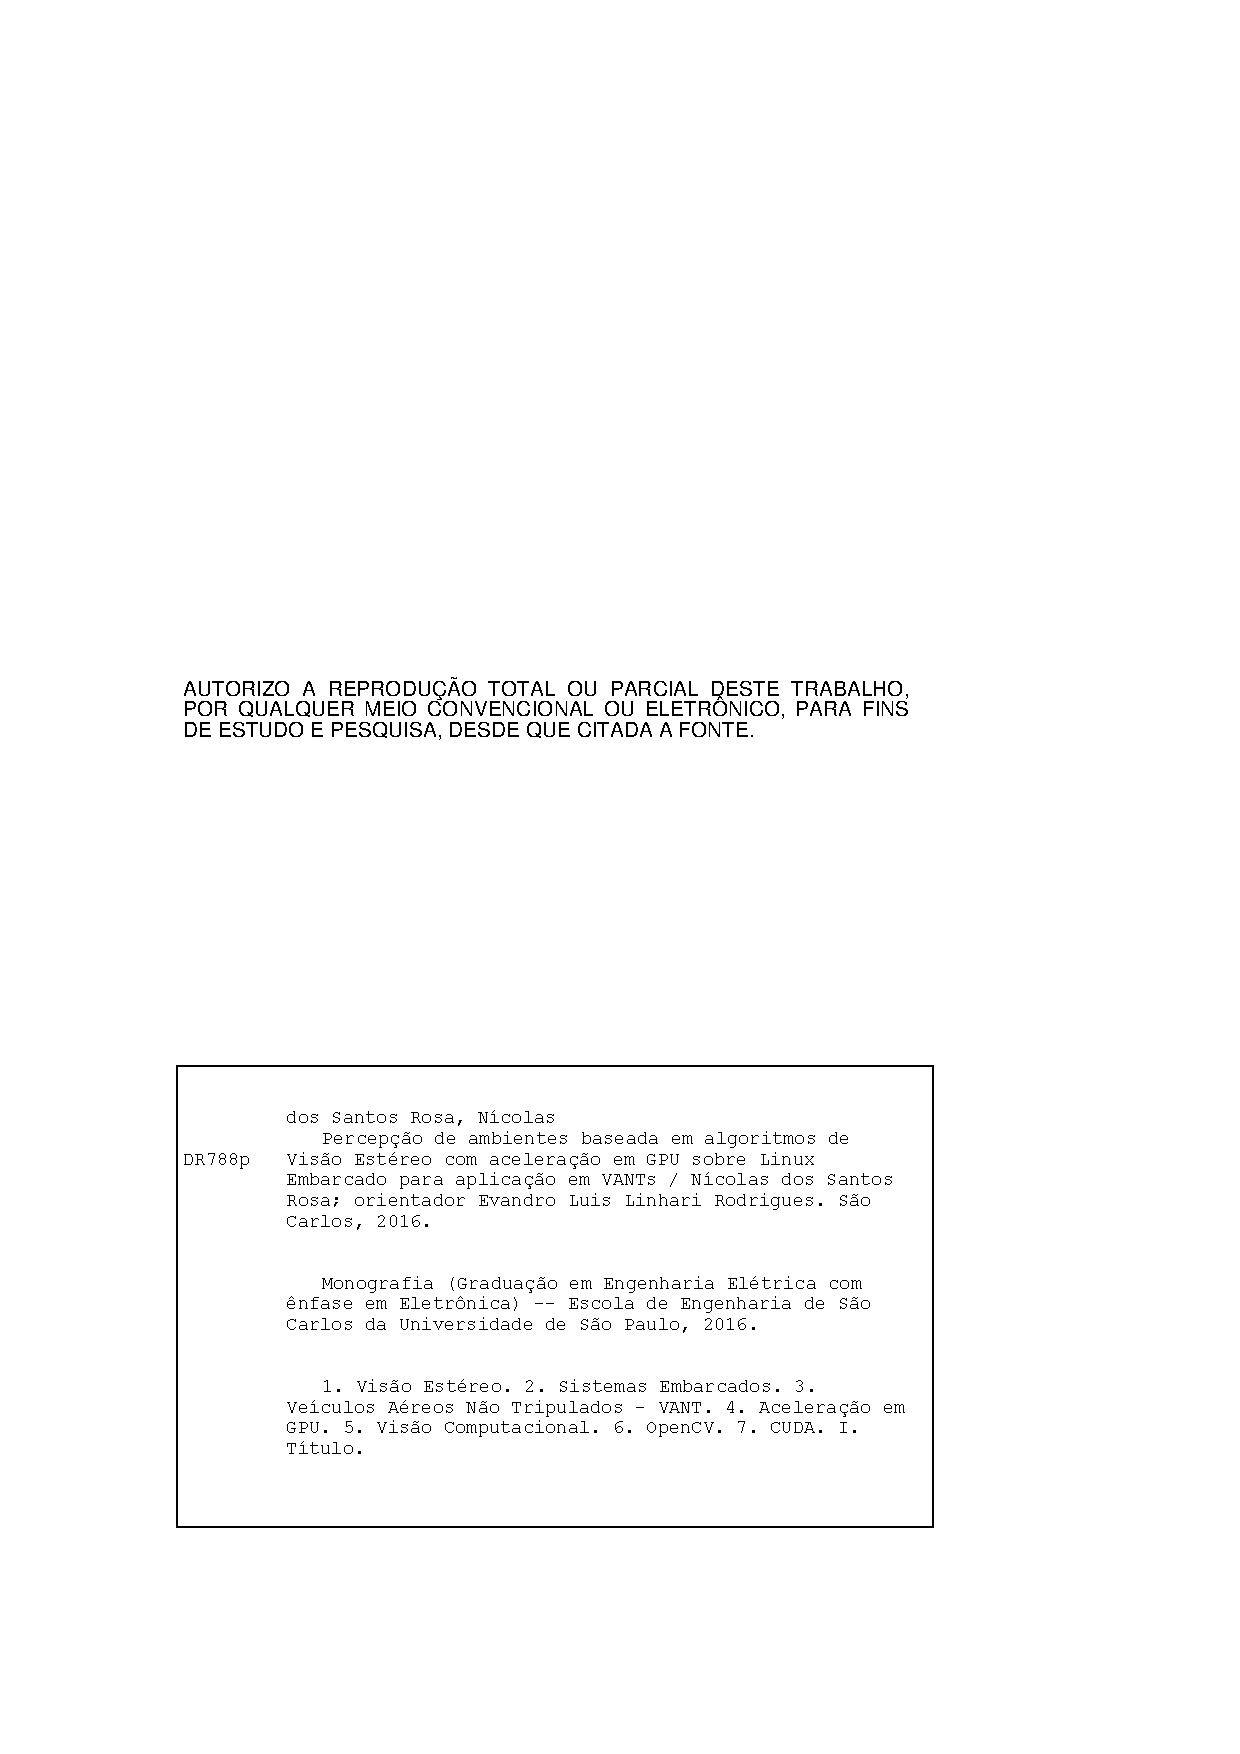
\includepdf{./Resources/ficha_catalografica.pdf}

%------------------------------------- Folha de aprovação--------------------------------------------
\newpage

página com a folha de aprovação (página ímpar). \cleardoublepage

\begin{comment}
\begin{figure}[H]
	\centering
	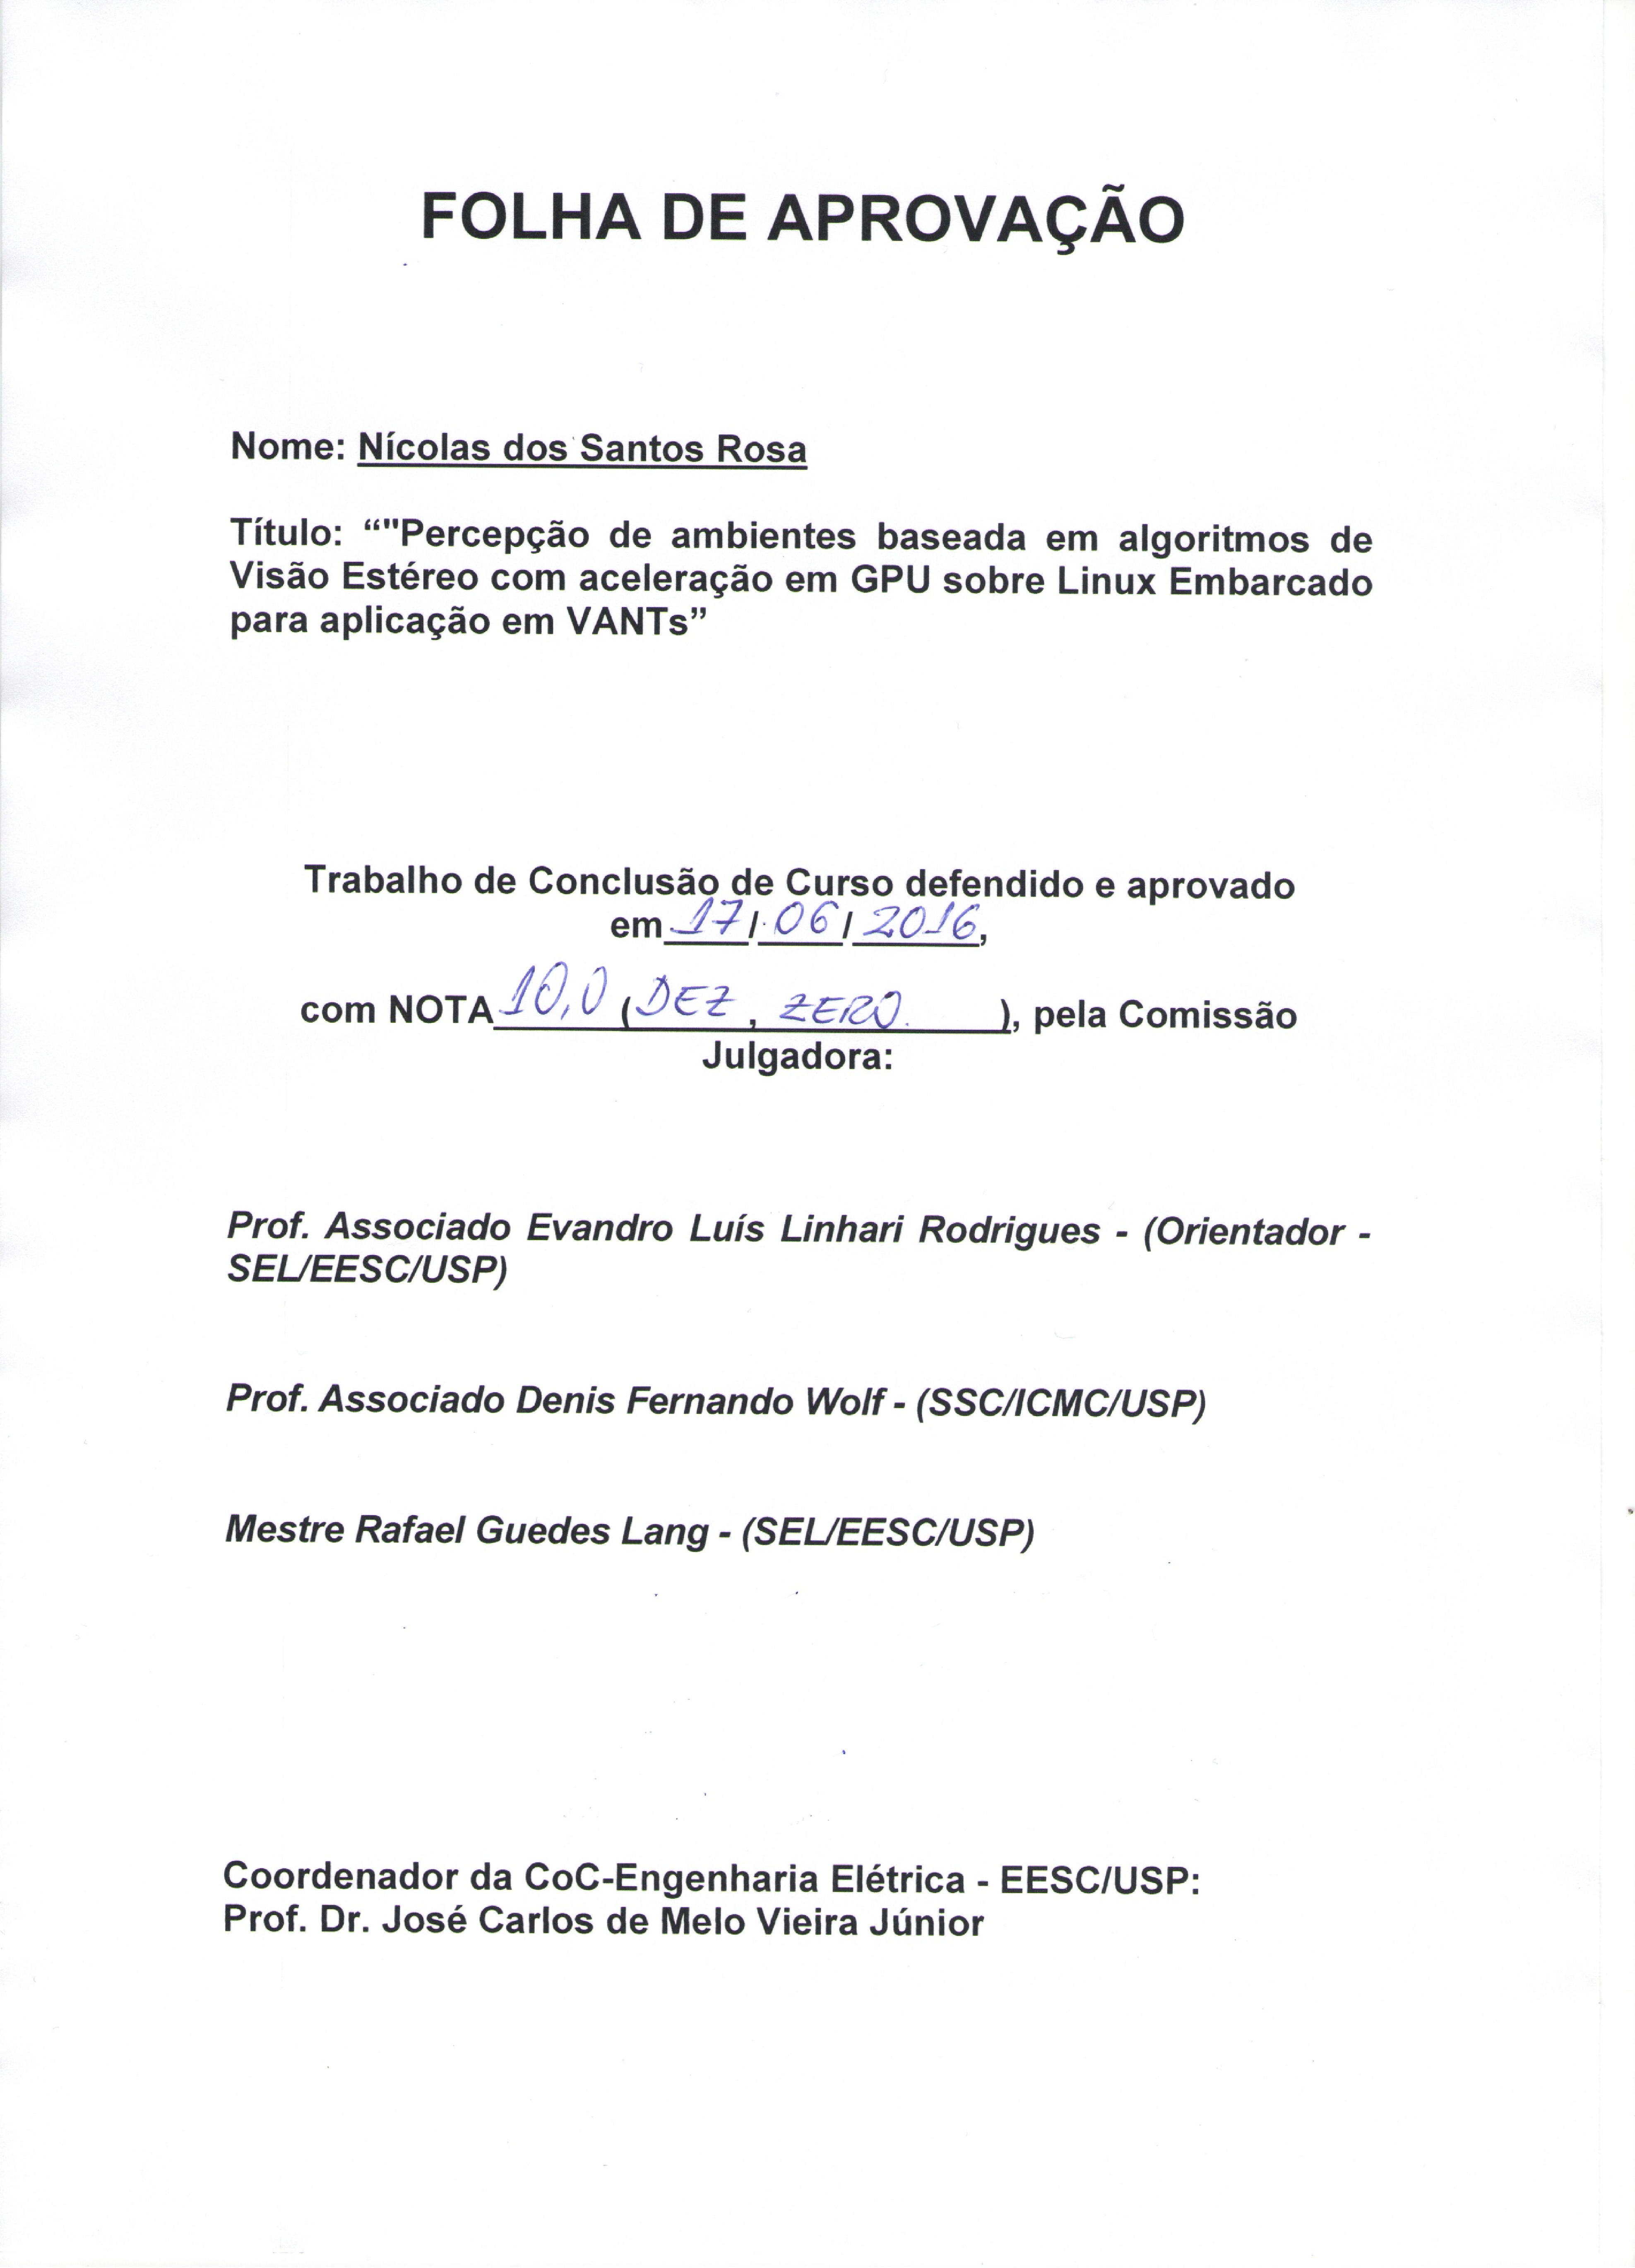
\includegraphics[scale=0.3]{./Resources/aprovacao.jpg}
	\caption{Fluxo de comunicação entre os principais componentes.}
	\label{Aprovacao}
\end{figure}
\cleardoublepage
\end{comment}
%------------------------------------- Dedicatória --------------------------------------------------
\vspace{0.11\textheight} 
\begin{center}
\textbf{\Huge{Dedicatória}}
\end{center}
\vspace{0.05\textheight}

Este trabalho de conclusão de curso é dedicado à minha mãe, ao meu pai, à minha irmã, aos meus padrinhos e a toda minha família.

\begin{flushright}
Nícolas dos Santos Rosa.
\end{flushright}

%------------------------------------- INSERÇÃO PÁGINA EM BRANCO ------------------------------------
\cleardoublepage

%------------------------------------- Agradecimentos -----------------------------------------------
\vspace{0.11\textheight} 

\begin{center}
\textbf{\Huge{Agradecimentos}}
\end{center}

\vspace{0.05\textheight}

Primeiramente, agradeço a Deus por propiciar saúde e felicidade a todos aqueles que me rodeiam.

À minha família: à minha mãe, Valdenilce, pela ferrenha dedicação em mostrar a mim e a minha irmã a importância da educação para nossa formação pessoal; ao meu pai, Francisco, por fazer o possível e o impossível para sustentar nossa família e por possibilitar condições para que me tornasse engenheiro; à minha irmã, Natália, pelo suporte e carinho e por ser a dupla perfeita para atazanar nossos pais; às minhas tias, Elisabeth, Vera Lúcia e Maria Regina, por serem minhas segundas mães, visto o tamanho do suporte, preocupação, e apreço dado. 

Ao meu orientador, Prof. Evandro Luís Linhari Rodrigues, pelo apoio para o desenvolvimento deste trabalho e por despertar meu interesse em sistemas embarcados, confirmando ainda mais minha paixão pelo meu curso.  

Aos meus orientadores de iniciação científica, Prof. Dr. Cláudio F. M. Toledo e Márcio S. Arantes, por introduzir-me ao âmbito da pesquisa acadêmica. Aos membros do SARLab: ao Prof. Dr. Samir Rawashdeh por ser o idealizador deste trabalho e por oferecer a oportunidade de desenvolvê-lo; a Benjamin Dale e a Miguel Rocha Jr., pelo companheirismo e por sempre estarem sempre de prontidão.

Aos meus amigos de curso, pelos ótimos momentos que vivemos juntos nestes anos, especialmente, Alexandre B. Moretti, Leonardo B. Farçoni, Plínio G. B. Ferreira, Marília L. Dourado,  Jéssica B. da Vida, Pedro Arantes, Augusto Martins, Gustavo Oliveira, Aline Midori, Vitor Martins, Anderson M. Tsai, Victor Morini, João F. Corsini, Caio Martins e a todos os outros amigos. 

Aos membros do grupo extracurricular Warthog Robotics, por partilhar um interesse em comum e pelas incontáveis horas de dedicação gastas no laboratório.

Por fim, agradeço a todos os envolvidos no desenvolvimento deste trabalho.

\begin{flushright}
Nícolas dos Santos Rosa.
\end{flushright}


%------------------------------------- INSERÇÃO PÁGINA EM BRANCO ------------------------------------
\cleardoublepage

%------------------------------------- EPÍGRAFE -----------------------------------------------------
\
\vspace{0.76\textheight} 

\begin{flushright}

\textit{"O dinheiro faz homens ricos, o conhecimento faz homens }

\textit{sábios e a humildade faz grandes homens."}

Mahatma Gandhi

\textit{"You can't put a limit on anything. The more you dream, the farther you get."}

Michael Phelps

\textit{"Se eu vi mais longe, foi por estar sobre ombros de gigantes."}

Isaac Newton

\end{flushright}


%------------------------------------- INSERÇÃO PÁGINA EM BRANCO ------------------------------------
\cleardoublepage

%------------------------------------- Resumo - Português -------------------------------------------
\vspace{0.11\textheight} 

\begin{center}
\textbf{\Huge{Resumo}}
\end{center}

\vspace{0.05\textheight}

Rosa, Nícolas \textbf{Mapeamento de ambientes baseado em algoritmos de visão estéreo para VANTs sobre Linux Embarcado}. Trabalho de Conclusão de Curso -- Escola de Engenharia de São Carlos, Universidade de São Paulo, 2016.

\vspace{0.05\textheight}

Atualmente, veículos aéreos não tripulados (VANT) vêm tornando-se um assunto recorrente no âmbito científico. Estes veículos, devido a sua mobilidade e inteligência artificial, vêm sendo adaptados para a atuação em diferentes ambientes, desempenhando assim diversas atividades que vão desde aplicações militares, agronômicas, espaciais, cinematográficas, entre outras. Entretanto, essa atuação só não é mais ampla devido a problemas relacionados ao reconhecimento do ambiente ao seu redor e detecção de objetos e obstáculos. Neste trabalho, estudou-se a utilização de visão estéreo em sistemas embarcados para mapeamento de ambientes e obstáculos ameacem a locomoção do veículo autônomo. Os métodos estéreo mais conhecidos pela literatura, BM (\textit{Block Matching}) e SGBM (\textit{Semi-Global Block Matching}), foram implementados e também foi desenvolvido uma interface que facilite a extração de informações e a comparação de performance destes métodos. Após análise, o algoritmo mais robusto para a aplicação em veículos aéreos foi o método BM para ambas as plataformas, BBB e \textit{Jetson TK1}. Visto que a \textit{Jetson TK1} permite a aceleração em hardware do método BM, foi possível implementar o método BMGPU (\textit{Block Matching with GPU Acceleration}) fornecido pelo OpenCV nesta plataforma. Por fim, os algoritmos utilizados permitiram que as distâncias de objetos próximos ao veículo móvel pudessem ser estimadas.

\vspace{0.05\textheight}

Palavras-Chave: Visão estéreo, Detecção de Obstáculos, Sistemas Embarcados, Veículos Aéreos Não Tripulados - VANT, Visão Computacional, OpenCV, Aceleração em GPU, CUDA.


%------------------------------------- INSERÇÃO PÁGINA EM BRANCO ------------------------------------ 
\cleardoublepage


%------------------------------------- Resumo - Inglês ----------------------------------------------
\vspace{0.11\textheight} 

\begin{center}
\textbf{\Huge{Abstract}}
\end{center}

\vspace{0.05\textheight}

Rosa, Nícolas \textbf{Environment Mapping based on Stereo Vision algorithms for UAVs on Embedded Linux}. Completion of course work -- São Carlos School of Engineering, University of São Paulo, 2016.

\vspace{0.05\textheight}

Currently, Unmanned Aerial Vehicles (UAV) are becoming a recurring theme in the scientific realm. These vehicles, because of their mobility and artificial intelligence, have been adapted to perform in different environments, thus performing various activities ranging from
military applications, agronomic, spacial, cinematographic, among others. However, this performance is not wider due to  problems related to the recognition of the surrounding environment and the detection objects and obstacles.In this work, it was studied the use of stereoscopic vision in embedded systems for environment mapping and obstacles that threaten the mobility of the autonomous vehicle. The most well known stereo methods in the literature, BM (\textit{Block Matching}) and SGBM (\textit{Semi-Global Block Matching}) were implement and was developed a graphical user interface, which facilitates the extraction of the information and comparing performance of these methods. After analysis, the most robust algorithm for use in aerial vehicles was the BM method for both platforms, BBB and \textit{Jetson TK1}. Since the \textit{Jetson TK1} allows hardware acceleration of the method BM, it was possible to implement the method BMGPU (\textit{Block Matching with GPU Acceleration}) provided by OpenCV on this platform. Finally, the used algorithms allowed the distances of obstacles near the moving vehicle could be estimated.

\vspace{0.05\textheight}

Keywords: Stereo Vision, Obstacle Detection, Embedded Systems, Unmanned aerial Vehicle - UAV, Computational Vision, OpenCV, GPU Acceleration, CUDA.


%------------------------------------- INSERÇÃO PÁGINA EM BRANCO ------------------------------------
\cleardoublepage

%------------------------------------- CONFIGURAÇÕES DOS ÍNDICES ------------------------------------
%\clearpage
%\thispagestyle{empty}
\listoffigures % Índice de Figuras

\listoftables % Índice de Tabelas

%------------------------------------- INSERÇÃO PÁGINA EM BRANCO ------------------------------------ 
\cleardoublepage

%------------------------------------- LISTA DE ABREVIATURAS ----------------------------------------
\vspace{0.11\textheight} 

\textbf{\Huge{Siglas}}

\vspace{0.05\textheight}

\begin{tabbing}
\hspace*{0.5cm}\=\hspace{2.5cm}\= \kill

% Lista de Abreviaturas
\> AAVC		\> \textit{Autonomous Aerial Vehicle Competition}									\\
\> AFRL		\> \textit{Air Force Research Laboratory} - Laboratório de pesquisas da Força Aérea Americana 				\\ 
\> ALU		\> \textit{Arithmetic Logic Unit} - Unidade Lógica e Aritmética				 				\\ 
\> ANAC		\> Agência Nacional de Aviação Civil 											\\
\> API		\> \textit{Application Programming Interface} - Interface de Programação de Aplicações					\\
\> AUV		\> \textit{Autonomous Underwater Vehicle} - Veículo Submarinos Autônomo	 						\\
\> BBB		\> \textit{BeagleBone Black}	 											\\
\> BM		\> \textit{Block Matching} - Método Estéreo Local	 								\\
\> BMGPU	\> \textit{Block Matching with GPU Acceleration} - 									\\
\>		\> Método Estéreo Local com Aceleração de GPU										\\
\> CPU		\> \textit{Central Processing Unit} - Unidade central de Processamento							\\
\> CUDA		\> \textit{Compute Unified Device Architecture} - Plataforma de computação paralela					\\
\> DECEA	\> Departamento de Controle do Espaço Aéreo										\\
\> FAA	 	\> \textit{Federal Aviation Administration} - Administração Federal de Aviação						\\
\> FPGA  	\> \textit{Field-programmable gate array} - Arranjo de Portas Programável em Campo					\\
\> FPS  	\> \textit{Frames per Second} - Quadros por Segundo									\\
\> GUI 	 	\> \textit{Graphical User Interface} - Interface gráfica do usuário							\\
\> GPU 	 	\> \textit{Graphics Processing Unit} - Unidade de Processamento Gráfico							\\
\> GPGPU 	\> \textit{General Purpose Graphics Processing Unit} -  								\\
\>		\> Unidade de Processamento Gráfico de Propósito Geral									\\
\> GPS 	 	\> \textit{Global Positioning System} - Sistema de Posicionamento Global						\\
\> LIDAR 	\> \textit{LIght Detection And Ranging}											\\
\> LMR 	 	\> Laboratório de Robótica Móvel											\\
\> MAVS  	\> \textit{Micro Air Vehicle} - Micro Veículo Aéreo									\\
\> MIT 	 	\> \textit{Massachusetts Institute of Technology}									\\
\> OACI  	\> Organização de Aviação Civil Internacional 										\\
\> RPA 	 	\> \textit{Remotely Piloted Aircraft} - Aeronave Remotamente Pilotada							\\
\> RTOS	 	\> \textit{Real-Time Operating System} - Sistema Operacional em Tempo Real						\\
\> SGBM  	\> \textit{Semi-Global Block Matching} - Método Estéreo Semi-global							\\
\> SIMD  	\> \textit{Single Instruction, Multiple Data}										\\
\> SLAM  	\> \textit{Simultaneous Localization and Mapping} - Localização e Mapeamento Simultâneo					\\
\> UAV/VANT 	\> \textit{Unmanned aerial vehicle} - Veículo Aéreo não tripulados 							\\

\end{tabbing}
\cleardoublepage
%------------------------------------- CONFIGURAÇÕES DOS ÍNDICES ------------------------------------ 
%\usepackage{fancyhdr}
\pagestyle{fancy}
\fancyhf{} % clear all header and footer fields
\fancyhead[RO, LE] {\thepage}

\fancypagestyle{plain}{\pagestyle{fancy}}

\tableofcontents % Índice Geral


%------------------------------------- Adição dos Capítulos -----------------------------------------	
\chapter{Introdu��o}
\label{Introducao}

A pesquisa em VANTs -- Ve�culos A�reos n�o Tripulado vem se tornando um assunto recorrente no �mbito cient�fico. A real motiva��o para seu desenvolvimento levanta diversas quest�es �ticas e legais, visto que foram inicialmente motivados para fins militares. Por outro lado, esse tipo de plataforma tamb�m possui aplica��es tais como: cultivo e pulveriza��o de culturas, produ��o cinematogr�fica, opera��es de busca e salvamento, inspe��o de linhas el�tricas de alta tens�o, entrega de mercadorias e encomendas.

A navega��o de um micro ve�culo a�reo em espa�o confinado � um desafio significante. Atualmente, a navega��o aut�noma enfrenta o problema de localiza��o e mapeamento simult�neo, mais conhecido como SLAM (Simultaneous Localization and Mapping) \cite{Dissanayake2001}. SLAM apresenta quatro etapas: Mapeamento, Percep��o, Localiza��o e Modelagem. A complexidade deste problema encontra-se no fato de que o ve�culo necessita navegar em um espa�o desconhecido, extrair caracter�sticas importantes do ambiente, construir um mapa com os dados obtidos e simultaneamente localizar-se dentro deste. O sensoriamento pode ser realizado tanto por Vis�o computacional ou por sensores �pticos. 

A proposta deste Trabalho de conclus�o de Curso � auxiliar o primeiro passo de Mapeamento de ambientes atrav�s de vis�o estereosc�pica. Este trabalho, � motivado a tentativa de reproduzir-se o desafio proposto pela Autonomous Aerial Vehicle Competition (AAVC)\cite{AAVC}, competi��o organizada pelo Laborat�rio de Pesquisas da Forca A�rea Americana (AFRL) e sediada em Dayton-OH. Esta competi��o incentiva o estudo de ve�culos a�reos aut�nomos, convidando diversas universidades a compartilhar seus avan�os nesta �rea de pesquisa. O competidor � motivado a adaptar um modelo de quadric�ptero 3DRobotics�, assim este ve�culo precisa cumprir um certo percurso com caixas como obst�culos,detectar e reportar � esta��o base a posi��o de um objeto.

O processo de desenvolvimento do ve�culo consiste em quatro passos: estrutura, circuito, controle e navega��o. Os dois primeiros itens comp�em o hardware, o qual estabelece as conex�es f�sicas necess�rias para integrar os sistemas de alimenta��o, comunica��o e controle. A parte de software engloba o desenvolvimento de algoritmos visando o controle e navega��o, mais especificamente o desenvolvimento do c�digo para Vis�o Est�reo (Stereo Vision) \cite{Lemaire2007}, planejamento de caminho (Path Planning) e arquitetura de m�quina de estados (Decision Making).

Um sistema aut�nomo tamb�m implica o processamento de imagens ser embarcado, isto �, o processamento para a navega��o do ve�culo ser realizada \textit{On-line}. Deste modo, as plataformas de desenvolvimento BeagleBone Black e Nvidia jetson TK1 ser�o analisadas e avaliadas com rela��o performance ao executar o algoritmo desenvolvido \cite{Shah2014}. 

\textcolor{red}{-----------------------------------------------------------------------------------------------}

Refer�ncia \cite{referencia1}.

Outra refer�ncia para a bibliografia \cite{referencia2}.

Refer�ncia para a figura \ref{logo}.

 \begin{figure}[H]
 	\centering
 	
\includegraphics[scale=0.35]{./Resources/latex-logo.png}
 	\caption{Logo do LaTeX.}
 	\label{logo}
 \end{figure}


% % % % % % % % % % % % % % % % % % % % % % % % % % % % % % % % % % % % % % % % % % % % % % % % % % %
\section{Objetivos}
\textcolor{red}{\textbf{Dica:} Apresente "somente" os objetivos - podem ser gerais e/ou espec�ficos}

\textcolor{red}{
\begin{enumerate}
	\item Desenvolvimento de um algoritmo de controle para ve�culo a�reo aut�nomo
	\item Estudo e aplica��o do algoritmo de localiza��o e mapeamento simult�neo baseado em Vis�o (Vision-based SLAM)
	\item Desenvolvimento de c�digo da Vis�o do Quadric�ptero para Linux Embarcado
	\item Utiliza��o da Plataforma ROS (Robot Operating System)
	\item Reproduzir o desafio proposto pela AAVC Competition	
\end{enumerate}
}
% % % % % % % % % % % % % % % % % % % % % % % % % % % % % % % % % % % % % % % % % % % % % % % % % % %
\section{Justificativa}
\textcolor{red}{\textbf{Dica:} Explana��o sobre porque o trabalho se
justifica e quais os pontos de relev�ncia do mesmo}

% % % % % % % % % % % % % % % % % % % % % % % % % % % % % % % % % % % % % % % % % % % % % % % % % % %
\section{Motiva��o}
\textcolor{red}{\textbf{Dica:} Um pequeno texto sobre o que motivou o desenvolvimento do
Trabalho}

% % % % % % % % % % % % % % % % % % % % % % % % % % % % % % % % % % % % % % % % % % % % % % % % % % %
\section{Organiza��o do trabalho}
\textcolor{red}{\textbf{Dica:} Apresente o que tem em cada cap�tulo.}































%-----------------------------------------------------------------------------------------------------------------------------------------------------------------------------------------------
% Embasamento Teórico ou Fundamentação Teórica: revisão da literatura dos tópicos que sustentam a ciência e o conhecimento, relativos aos objetivos e aos métodos escolhidos para o desenvolvimento do trabalho.
% Itens como Considerações Iniciais e Finais não são obrigatórios, mas completam muito bem qualquer capítulo.
\chapter{Fundamentos Teóricos}
\label{Revisão Bibliográfica}

A visão estéreo possibilita a identificação de um espaço tridimensional, visto que sua estrutura permite a triangulação de pontos chaves, assim determinando o seu correto posicionamento. Deste modo, compreende-se o porquê deste sistema visual ser amplamente difundido na evolução humana e animal. Em visão computacional, deseja-se emular os sistemas de visão mais eficientes para identificação de objetos e reconhecimento de ambientes. Este processo pode ser realizado  computacionalmente, porém com alguns conceitos como Triangulação, Geometria Epipolar, Calibração e Retificação e Correspondência Estéreo. Estes conceitos encontram-se apresentados nas próximas seções.


%-----------------------------------------------------------------------------------------------------------------------------------------------------------------------------------------------
\section{Visão Estéreo - \textit{Stereo Vision}}
\subsection{Triangulação - \textit{Triangulation}}

Idealmente, a triangulação de um ponto P de coordenadas globais $(X,Y,Z)$ pode ser realizada caso tenha-se uma estrutura estéreo, cujas lentes não apresentem distorção e estejam perfeitamente alinhadas. Deste modo, matematicamente, é possível abstrair os sensores das câmeras como dois planos coplanares entre si. Nessas condições, tem-se que os eixos ópticos das câmeras são paralelos. O eixo óptico, também conhecido como raio principal, é a reta que intercepta o ponto de centro de projeção ${O}$ e o ponto principal da lente ${c}$. Assumindo que as câmeras sejam exatamente iguais e alinhadas, tem-se que os pontos focais da câmera esquerda e da câmera direita são iguais ${f_l = f_r}$ e os pontos principais ${c^{left}_x}$ e  ${c^{right}_x}$ apresentam as mesmas coordenadas \cite{Bradski2008}. A figura \ref{stereo_image_geometric_model} ilustra a representação do modelo idealizado de um sistema estéreo.

\begin{figure}[H]
 	\centering
 	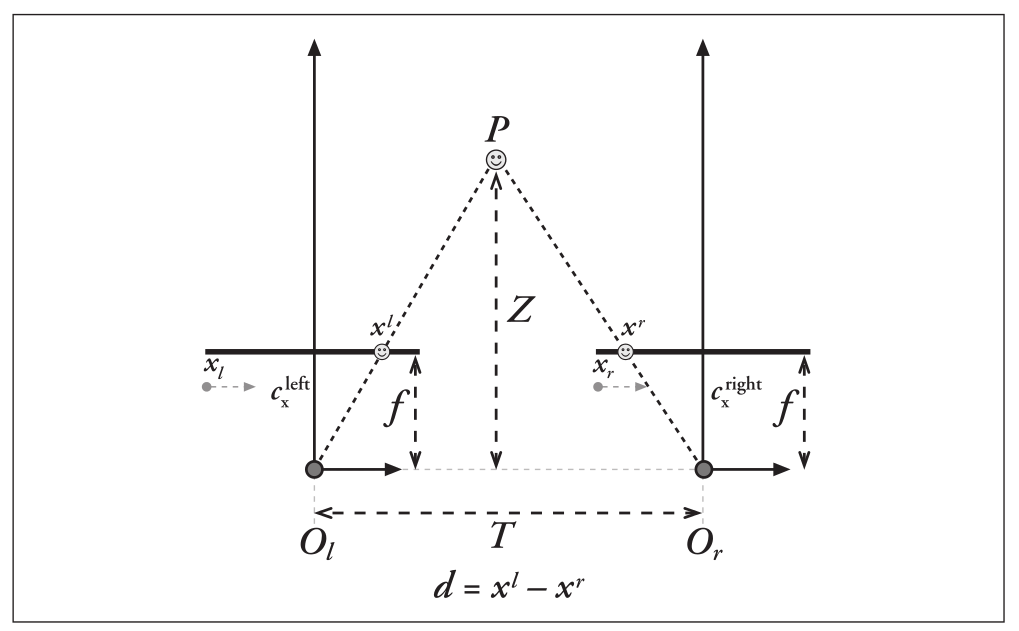
\includegraphics[scale=0.35]{./Resources/bradski/stereo_image_geometric_model.png}
 	\caption{Modelo Idealizado de um sistema de visão estéreo. Imagem retirada de \cite{Bradski2008}.}
 	\label{stereo_image_geometric_model}
\end{figure}

A distância presente entre os pontos $x^l$ e $x^r$ é dada pela equação $d = x^l - x^r$, o valor de $d$ é comumente também de chamado de disparidade. Caso os pontos $x^l$ e $x^r$, a distância focal $f$, a distância entre os centros das câmeras $(T,baseline)$ sejam conhecidos é possível determinar a distância entre o ponto P à base das câmeras $(Z)$. Por meio de semelhanças de triângulos, é possível estabelecer uma relação entre os triângulos $O_lPO_r$ e $x^lPx^r$, a qual está apresentada na equação \ref{triangle_similarity}.

\begin{equation}
\label{triangle_similarity}
\frac{T - (x^l-x^r)}{Z-T} = \frac{T}{Z} \Rightarrow Z = \frac{fT}{(x^l-x^r)} = \frac{fT}{d}
\end{equation}


%-----------------------------------------------------------------------------------------------------------------------------------------------------------------------------------------------
\subsection{Geometria epipolar - \textit{Epipolar Geometry}}

Geometria epipolar corresponde à estrutura básica de um sistema estéreo, na qual leva em consideração os modelos \textit{pinhole} de ambas câmeras utilizadas e encontra-se ilustrada pela figura \ref{geometry_epipolar}. 

\begin{figure}[H]
 	\centering
 	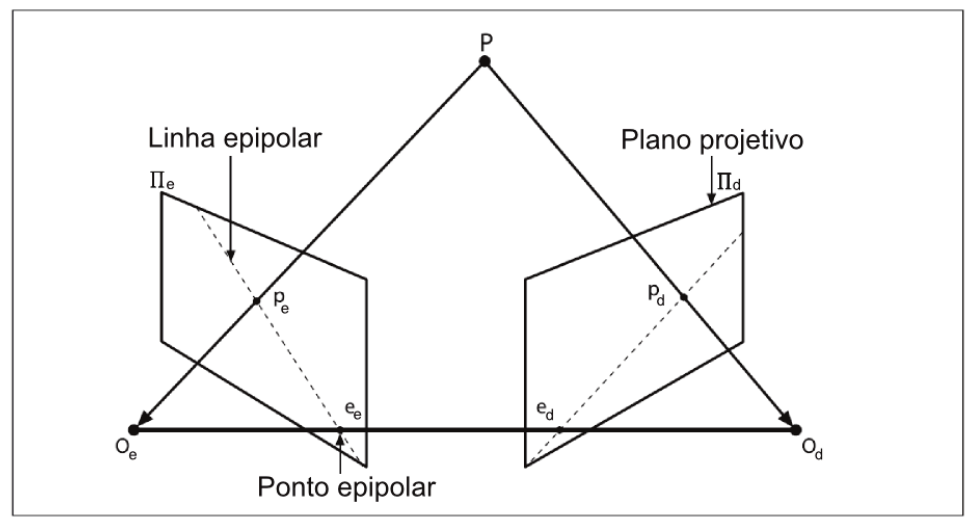
\includegraphics[scale=0.35]{./Resources/bradski/geometry_epipolar.png}
 	\caption{Exemplificação do caso típico de Geometria epipolar. Imagem retirada de \cite{Mendes2012}.}
 	\label{geometry_epipolar}
\end{figure}

Projeta-se o ponto P nos centros de projeção $O^e$ e $O^d$, as linhas que interligam o ponto P a esses centros interceptam os planos $\Pi_e$ e $\Pi_d$ nos pontos $p_e$ e $p_d$. Os pontos epipolares (\textit{epipoles}) $e_e$ e $e_d$ estão localizados nos pontos de intersecção da linha que interliga os centros de projeção e os planos projetivos \cite{Mendes2012}. O conhecimento desta geometria é importante pra o entendimento da chamada restrição epipolar (\textit{epipolar constraint}).

Considerando um sistema estéreo e um certo ponto $P$, deseja-se localizar na imagem da direita o seu ponto homólogo $P'$, isto é, sua projeção no plano projetivo direito. Sem a restrição, faz-se necessário a busca bidimensional em todo espaço do plano $\Pi_d$. Por outro lado, essa restrição garante que o ponto homólogo deve estar sobre a linha epipolar da imagem direita. Deste modo, é possível restringir a busca a uma única dimensão, busca somente sobre a linha epipolar, reduzindo consideravelmente o custo computacional \cite{Bradski2008}. Todavia, o sistema estéreo deve estar corretamente calibrado para que possa tomar mão desta restrição. Em visão computacional, a chamada matriz fundamental refere-se a matrix 3x3 utilizada para relacionar os pontos correspondentes do par de imagens estéreo. A expressão \ref{epipolar_constraint} que representa a restrição epipolar é dada pela relação entre a matriz fundamental F e os dois pontos correspondentes, em coordenadas de pixel \cite{RobertLaganiere}.

\begin{equation}
 \label{epipolar_constraint}
 p'^TFp = 0
\end{equation}


%-----------------------------------------------------------------------------------------------------------------------------------------------------------------------------------------------
\subsection{Calibração das Câmeras - \textit{Calibration}}
\label{theory_calib}

Até o presente momento, todos os conceitos apresentados assumiam que as câmeras são idealmente alinhadas e que suas lentes não apresentavam distorção. Na realidade, os centros ópticos não são perfeitamente alinhados e a lente introduz distorções à imagem projetada no sensor da câmera. Deste modo, faz-se necessário o processo de calibração, o qual mensura estas deformidades e estima os parâmetros que consigam anular ou minimizar estas imperfeições. Isso permite que os métodos computacionais obtenham resultados mais precisos. Estes parâmetros são classificados em dois tipos específicos: intrínsecos e extrínsecos.


%----------------------------------------------------------------------------------------------------------------------------------------------------------------------------------------------
\subsubsection{Parâmetros intrínsecos}

Correspondem às propriedades intrínsecas de cada câmera, as quais são descritas pela matriz M (\textit{Intrinsic Matrix}) e o vetor D (\textit{Distortion Coefficients Vector}). A figura \ref{lenses_distortion} ilustra o modelo completo, componente radial e componente tangencial do modelo de distorções das lentes da câmera esquerda e direita, respectivamente \cite{OpenCVCalibrationModule}.

\begin{equation}
 M = \begin{pmatrix}
f_x & 0   & c_x\\ 
  0 & f_y & c_y\\ 
  0 & 0   & 1
\end{pmatrix}
\end{equation}

\begin{center}
  $f_x,f_y$: Distância focal
  
  $c_x,c_y$: Compensação do ponto principal
\end{center}

\begin{equation}
  D = (k_1,k_2,p_1,p_2[,k_3[,k_4,k_5,k_6]])
\end{equation}

\begin{center}
  $k_1,k_2,k_3$: Coeficientes de distorção radial simétrica
  
  $p_1,p_2$: Coeficientes de distorção tangencial (descentrada)
\end{center}

%----------------------------------------------------------------------------------------------------------------------------------------------------------------------------------------------
\subsubsection{Parâmetros extrínsecos}
Correspondem às propriedades extrínsecas, isto é, demonstram a disposição espacial da segunda câmera, direita, com relação à câmera da esquerda em coordenadas globais. Assim como ilustrado na figura \ref{essential_geometry.png}, a matriz de rotação R (3x3) e o vetor de translação T (3x1) são responsáveis por descrever este deslocamento. Geralmente, quando o quadro de referência não se encontra no centro de projeção da câmera, faz-se necessário a adição da matriz de rotação e o vetor de translação. Neste contexto, utiliza-se o sistema de coordenadas homogêneas, isto é, pontos 2D são representados como vetores 3x1 e pontos 3D como vetores 4x1. Deste modo, tem-se que a equação \ref{projection_equation} descreve a relação do ponto $P(X,Y,Z)$ e o ponto projetado $p'$ no plano $\Pi_r$\cite{RobertLaganiere}.

%----------------------------------------------------------------------------------------------------------------------------------------------------------------------------------------------
\begin{equation}
  s.p' = M
  \begin{bmatrix}
  \begin{array}{c|c}
  R & t
  \end{array}
  \end{bmatrix}
  P 
\end{equation}

%----------------------------------------------------------------------------------------------------------------------------------------------------------------------------------------------
\begin{equation}
\label{projection_equation}
s
\begin{bmatrix}
x \\ 
y \\ 
1 
\end{bmatrix}
= 
\begin{bmatrix}
f_x & 0 & c_x\\ 
0 & f_y & c_y\\ 
0 & 0 & 1
\end{bmatrix} 
\begin{bmatrix}
r_{11} & r_{12} & r_{13} & t_1 \\ 
r_{21} & r_{22} & r_{23} & t_2 \\ 
r_{31} & r_{32} & r_{33} & t_3
\end{bmatrix}
\begin{bmatrix}
X \\ 
Y \\ 
Z \\ 
1
\end{bmatrix}
\end{equation}

%----------------------------------------------------------------------------------------------------------------------------------------------------------------------------------------------
\begin{figure}[H]
 	\centering
 	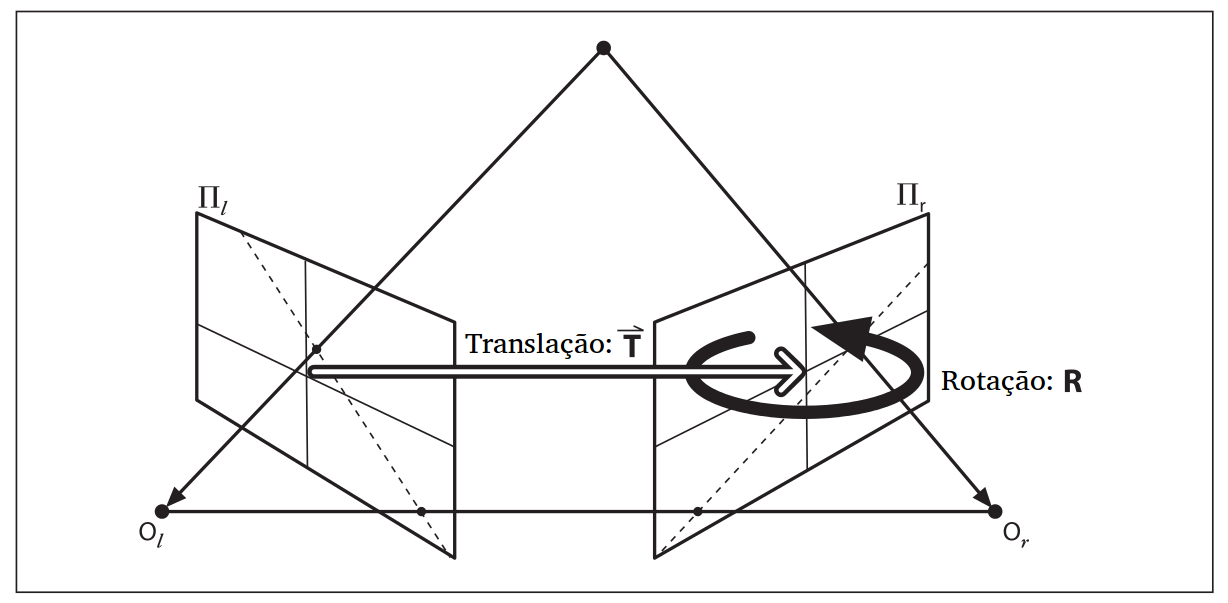
\includegraphics[scale=0.25]{./Resources/bradski/essential_geometry_ptbr.png}
 	\caption{O deslocamento do plano $\Pi_r$ com relação ao plano $\Pi_l$ pode ser descrito pela matriz R e o vetor de translação T. Imagem retirada de \cite{Bradski2008}.}
 	\label{essential_geometry.png}
\end{figure}

%----------------------------------------------------------------------------------------------------------------------------------------------------------------------------------------------
Devido ao desalinhamento entre as câmeras, torna-se necessário estimar estas variáveis, aumentando, assim, a eficiência dos métodos estéreo ao procurarem pelas correspondências entre as duas imagens. A figura \ref{stereo_calib_extrinsic}, ilustra o processo de calibração dos parâmetros extrínsecos, no qual utiliza-se um conjunto de imagens do padrão de calibração. Ao fim deste processo, é possível aferir o posicionamento da segunda câmera com relação à primeira \cite{Bouguet1999}.


%----------------------------------------------------------------------------------------------------------------------------------------------------------------------------------------------
\subsection{Retificação das Imagens - \textit{Rectification}}

O processo de retificação é responsável por realizar as correções com relação à distorção das lentes e ao alinhamento das câmeras, de acordo com os parâmetros obtidos pelo processo de calibração apresentado no tópico anterior. Ao fim deste processo, deseja-se que o par de imagens estéreo esteja retificado e sem distorções, preparado para a aplicação dos métodos estéreo, assim como ilustrado na figura \ref{rectification_process}.

\begin{figure}[H]
 	\centering
 	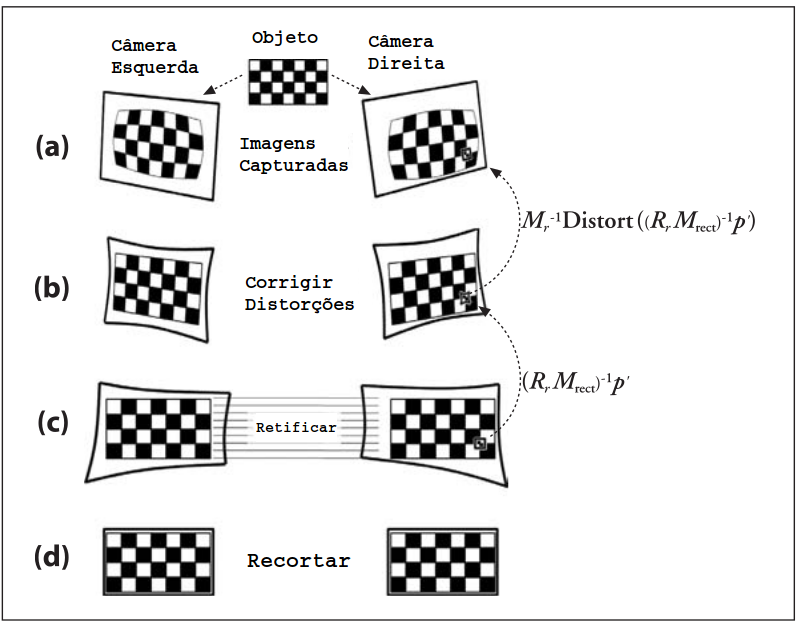
\includegraphics[scale=0.32]{./Resources/bradski/rectification_process_ptbr.png}
 	\caption{Retificação de Imagens - Processo de retificação estéreo. Imagem retirada de \cite{Bradski2008}.}
 	\label{rectification_process}
\end{figure}


%-----------------------------------------------------------------------------------------------------------------------------------------------------------------------------------------------
\subsection{Correspondência Estéreo - \textit{Stereo Correspondence}}

Correspondência estéreo não é nada mais que a utilização de métodos estéreo, os quais são responsáveis pela procura de pontos homólogos nos pares de imagens estéreo. Como visto anteriormente, devido ao distanciamento das câmeras $(T)$ e ao distanciamento do objeto com relação às câmeras $(Z)$, o mesmo ponto apresenta diferentes posicionamento nos planos das câmeras $x^l$ e $x^r$. A figura \ref{homologous_points _stereo} ilustra um par de imagens estéreo (esquerda e direita) e o mapa de disparidades gerado pela cena, nas quais os pixels homólogos estão destacados. Os métodos estéreo utilizam da restrição epipolar o que reduz o espaço de busca e de diferentes meios para encontrá-los. Mesmo com essa restrição e com a retificação das imagens, os métodos ainda assim apresentam um elevado custo computacional, além do que ainda estão sujeitos à encontrarem falsas correspondências \cite{Wang2007}. 

\begin{figure}[H]
 	\centering
 	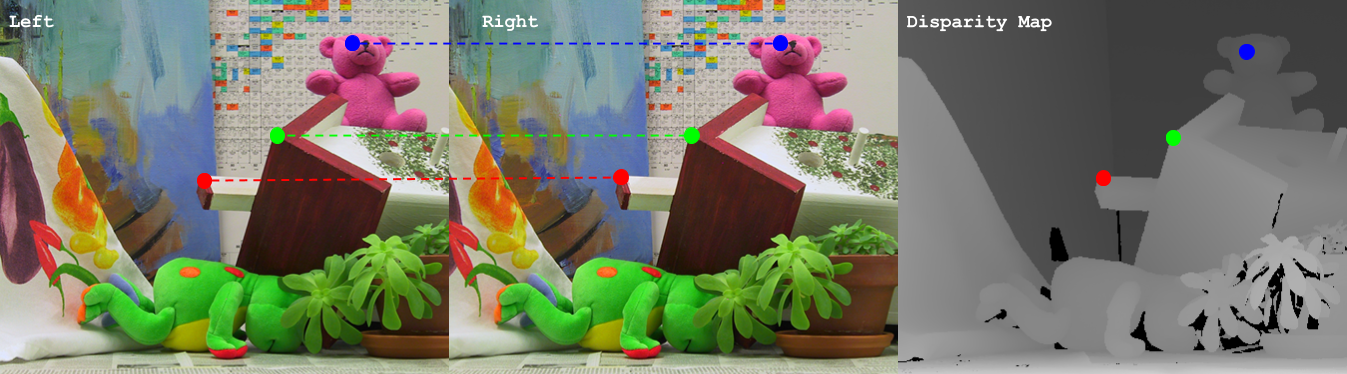
\includegraphics[scale=0.33]{./Resources/homologous_points_stereo.png}
 	\caption{Correspondência de pontos homólogos em um par de imagens estéreo. Imagem original retirada de \cite{Scharstein2003}.}
 	\label{homologous_points _stereo}
\end{figure}


%-----------------------------------------------------------------------------------------------------------------------------------------------------------------------------------------------
\subsubsection{Mapa de disparidades - \textit{Disparity Map}}

Como já foi dito anteriormente, disparidade é o deslocamento dos pontos homólogos entre as duas imagens. Nos métodos estéreo, o valor da disparidade é codificado em escala de cinza, a qual é inversamente proporcional à distância do objeto, assim como representado na figura \ref{depth_disparity}. Assim, níveis de cinza mais altos (tons claros) correspondem a disparidades maiores (perto) e níveis de cinza mais baixos (tons escuros) correspondem a disparidades mais baixas (distante). Devido a sua relação com a distância, este conceito é comumente atrelado à percepção de profundidade.

\begin{figure}[H]
 	\centering
 	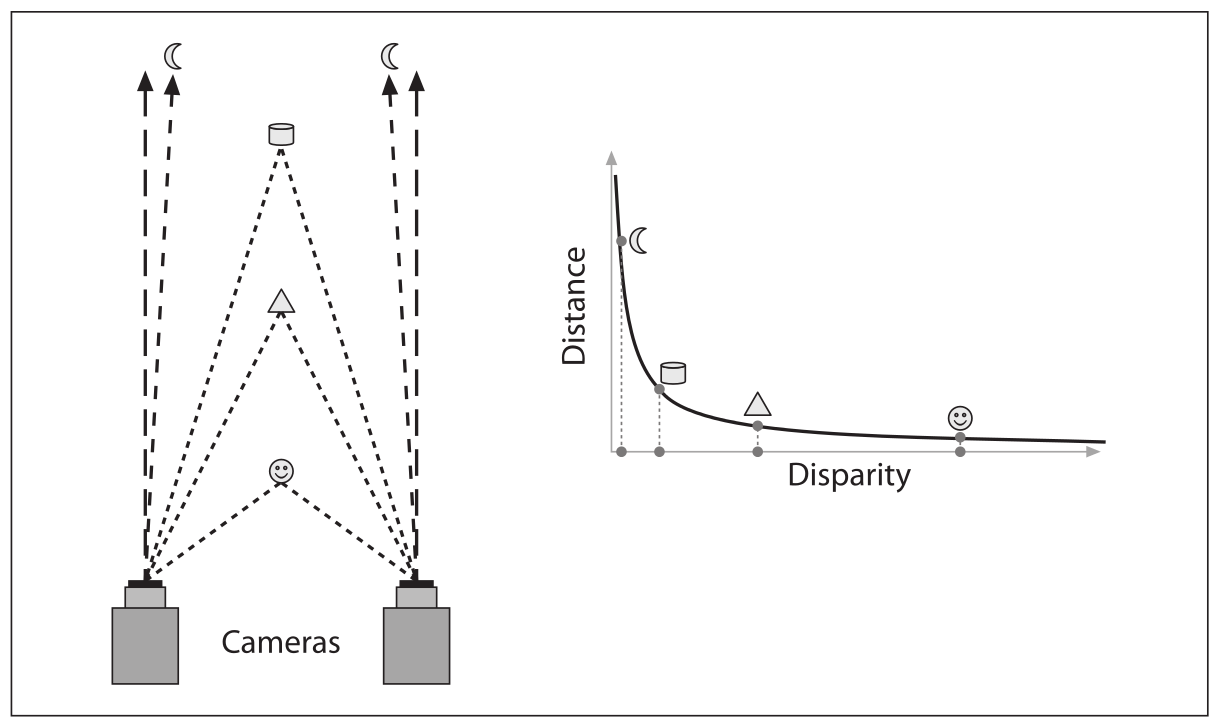
\includegraphics[scale=0.3]{./Resources/bradski/depth_disparity.png}
 	\caption{Relação inversamente proporcional entre distância e disparidade. Imagem retirada de \cite{Bradski2008}.}
 	\label{depth_disparity}
\end{figure}

%-----------------------------------------------------------------------------------------------------------------------------------------------------------------------------------------------
\subsubsection{Métodos Estéreo}
\label{stereo_methods}
A seguir, encontra-se apresentado um pequeno resumo de como são os operadores dos métodos estéreo utilizados neste trabalho.

\textbf{\textit{Block Matching} - BM:} Este algoritmo é um método local, no qual utiliza soma das diferenças ao quadrado (SSD - \textit{Sum of Squared Differences}) para a determinação de correspondências. O tamanho da vizinhança deve ser avaliado, visto que a densidade do mapa gerado, nível de detalhamento e intensidade de ruído dependem disso. Caso o bloco seja pequeno, o mapa apresentará detalhes mais nítidos, porém adicionará ruídos ao mapa. Por outro lado, um bloco maior reduz o nível de ruído, porém diminui o nível de detalhamento do mapa. As limitações serviram de motivação para a criação do método a seguir \cite{Hirschmuller2008}.   

\textbf{\textit{Semi-global Block Matching} - SGBM:} Este algoritmo é um método global e também visa a obtenção de uma correspondência estéreo mais precisa, para isso, além da etapa de agregação de custo (cálculo da similaridade), modela-se o sistema como um problema de minimização energética, o que adiciona restrições que suavizam o mapa ao penalizar descontinuidades.  \cite{JunhwanKim2003}. Por conta disso, este método é mais lento que o apresentado anteriormente, porém é mais denso ao comparar-se o nível de detalhamento para um bloco de tamanho pequeno \cite{Hirschmuller2008}.

\textbf{\textit{Block Matching with GPU Acceleration} - BMGPU:} Método é igual ao primeiro apresentado, diferindo do fato que as suas bibliotecas e métodos implementados são voltados para a aceleração em GPU (\textit{Graphics Processing Unit}). Dado o paralelismo inerente dos aceleradores gráficos de hoje, esse tipo de \textit{hardware} permite o processamento simultâneo dos dados. 


%-----------------------------------------------------------------------------------------------------------------------------------------------------------------------------------------------
\subsection{Aplicações em Robótica}
\label{aplicacoes_robotica}
Nesta seção, serão apresentados alguns dos trabalhos que têm como principais sensores câmeras estéreo para a navegação autônoma em ambientes terrestre, aérea e subaquática.

Nos dias de hoje, as empresas automobilísticas vêm participando de uma verdadeira corrida tecnológica para o desenvolvimento de automóveis totalmente autônomos e economicamente viáveis. As universidades não ficaram para trás e também apresentam pesquisas envolvendo desenvolvimento de algoritmos de controle e sensores, tornando essa corrida ainda mais acirrada. Os resultados apresentados são realmente promissores, e concretizam cada vez mais essa realidade tida até então como distante \cite{Howard2014}. Na figura \ref{caminhao_autonomo}, é possível observar o projeto de caminhão autônomo desenvolvido pelo Laboratório de Robótica Móvel - LRM - ICMC/USP. O caminhão conta com diversos sensores, dentre eles câmeras estéreo, que identificam outros automóveis, pessoas e faixas de sinalização \cite{ShinzatoP}. 


%-----------------------------------------------------------------------------------------------------------------------------------------------------------------------------------------------
\begin{figure}[]
 	\centering
 	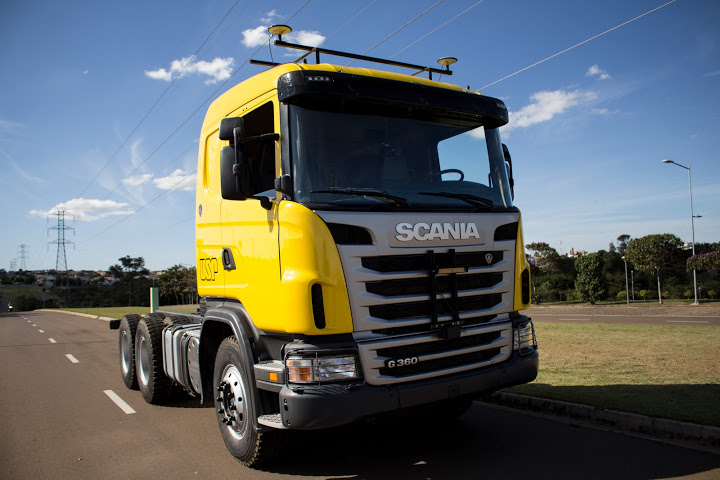
\includegraphics[scale=0.40]{./Resources/caminhao_autonomo.jpg}
 	\caption{Fotografia do caminhão autônomo desenvolvido pelo Laboratório de Robótica Móvel - LRM - ICMC/USP em parceria com a Scania.}
 	\label{caminhao_autonomo}
\end{figure}


%-----------------------------------------------------------------------------------------------------------------------------------------------------------------------------------------------
No caso de navegação autônoma para ambiente aéreo, o projeto utilizando \textit{Micro Air Vehicle} (MAVS) desenvolvido pelo \textit{Massachusetts Institute of Technology} (MIT) permite que pequenas aeronaves consigam navegar autonomamente e desviar de obstáculos voando a uma velocidade de 30 mph (48 $km/h$). A figura \ref{mit_drones} apresenta o trabalho desenvolvido, o qual é um comparativo de desempenho de uma implementação em hardware utilizando \textit{Field-programmable gate array} (FPGA) e um processador ARM para processamento embarcado do método SGBM \cite{BarryMIT}.


%-----------------------------------------------------------------------------------------------------------------------------------------------------------------------------------------------
\begin{figure}[]
 	\centering
 	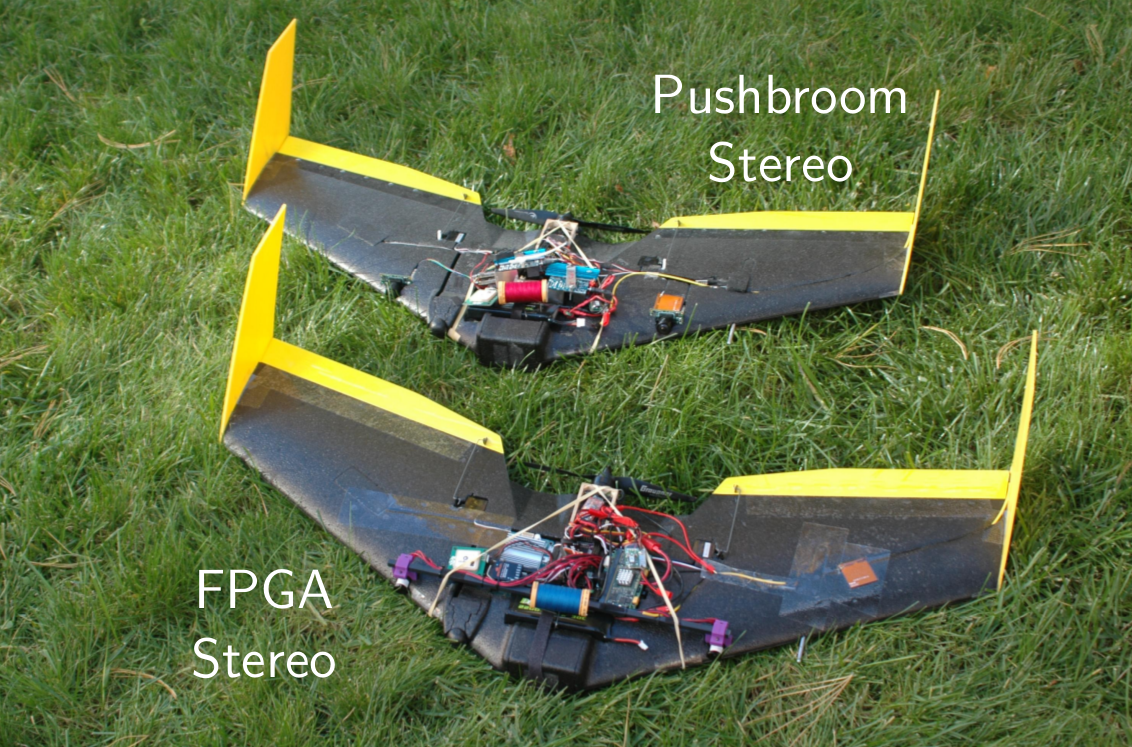
\includegraphics[scale=0.26]{./Resources/mit_drones.png}
 	\caption{Fotografia das plataformas experimentais de aeronaves utilizando Sistema Estéreo-FPGA e Sistema Estéreo-\textit{Pushbroom}. Câmeras são montados na parte dianteira das asas na mesma linha de base (34 cm) em ambas células. Imagem retirada de \cite{BarryMIT}.}
 	\label{mit_drones}
\end{figure}

Para atingir este objetivo, os pesquisados utilizaram uma arquitetura hídrida de sensores, como ilustrado na figura \ref{barry_diagram}, na qual os sensores visuais (câmeras estéreo) juntamente com os sensores para estimação de estado (Sensores Inerciais, Barômetro, Tubo de Pitot) permitem a construção da nuvem de pontos 3D do ambiente.

\begin{figure}[]
 	\centering
 	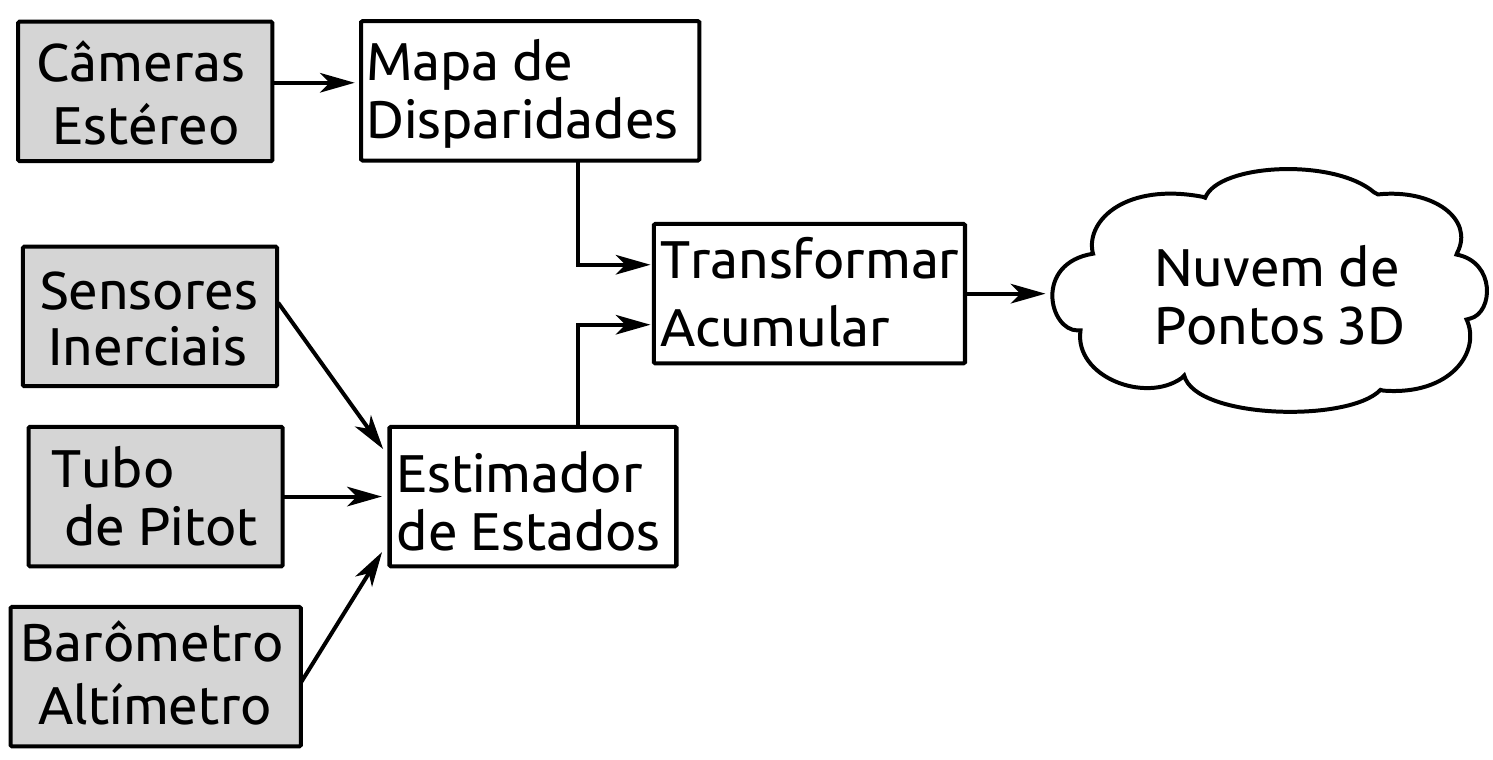
\includegraphics[scale=0.20]{./Resources/barry_diagram.png}
 	\caption{Visão geral da arquitetura utilizada nas aeronaves desenvolvidas pelos pesquisadores do MIT. Imagem traduzida de \cite{Barry2014}.}
 	\label{barry_diagram}
\end{figure}


%-----------------------------------------------------------------------------------------------------------------------------------------------------------------------------------------------
No caso de navegação autônoma para ambiente subaquático, um exemplo de \textit{autonomous underwater vehicle} (AUV) é o projeto desenvolvido pela Universidade espanhola de Girona (veja figura \ref{G500}). O trabalho propõe a utilização do método de Mapeamento e Localização Simultânea (SLAM), juntamente com câmera estéreo, para o reconhecimento do ambiente, aprimorando assim o erro de rastreamento dos objetos \cite{Nagappa2013}.


%-----------------------------------------------------------------------------------------------------------------------------------------------------------------------------------------------
\begin{figure}[H]
 	\centering
 	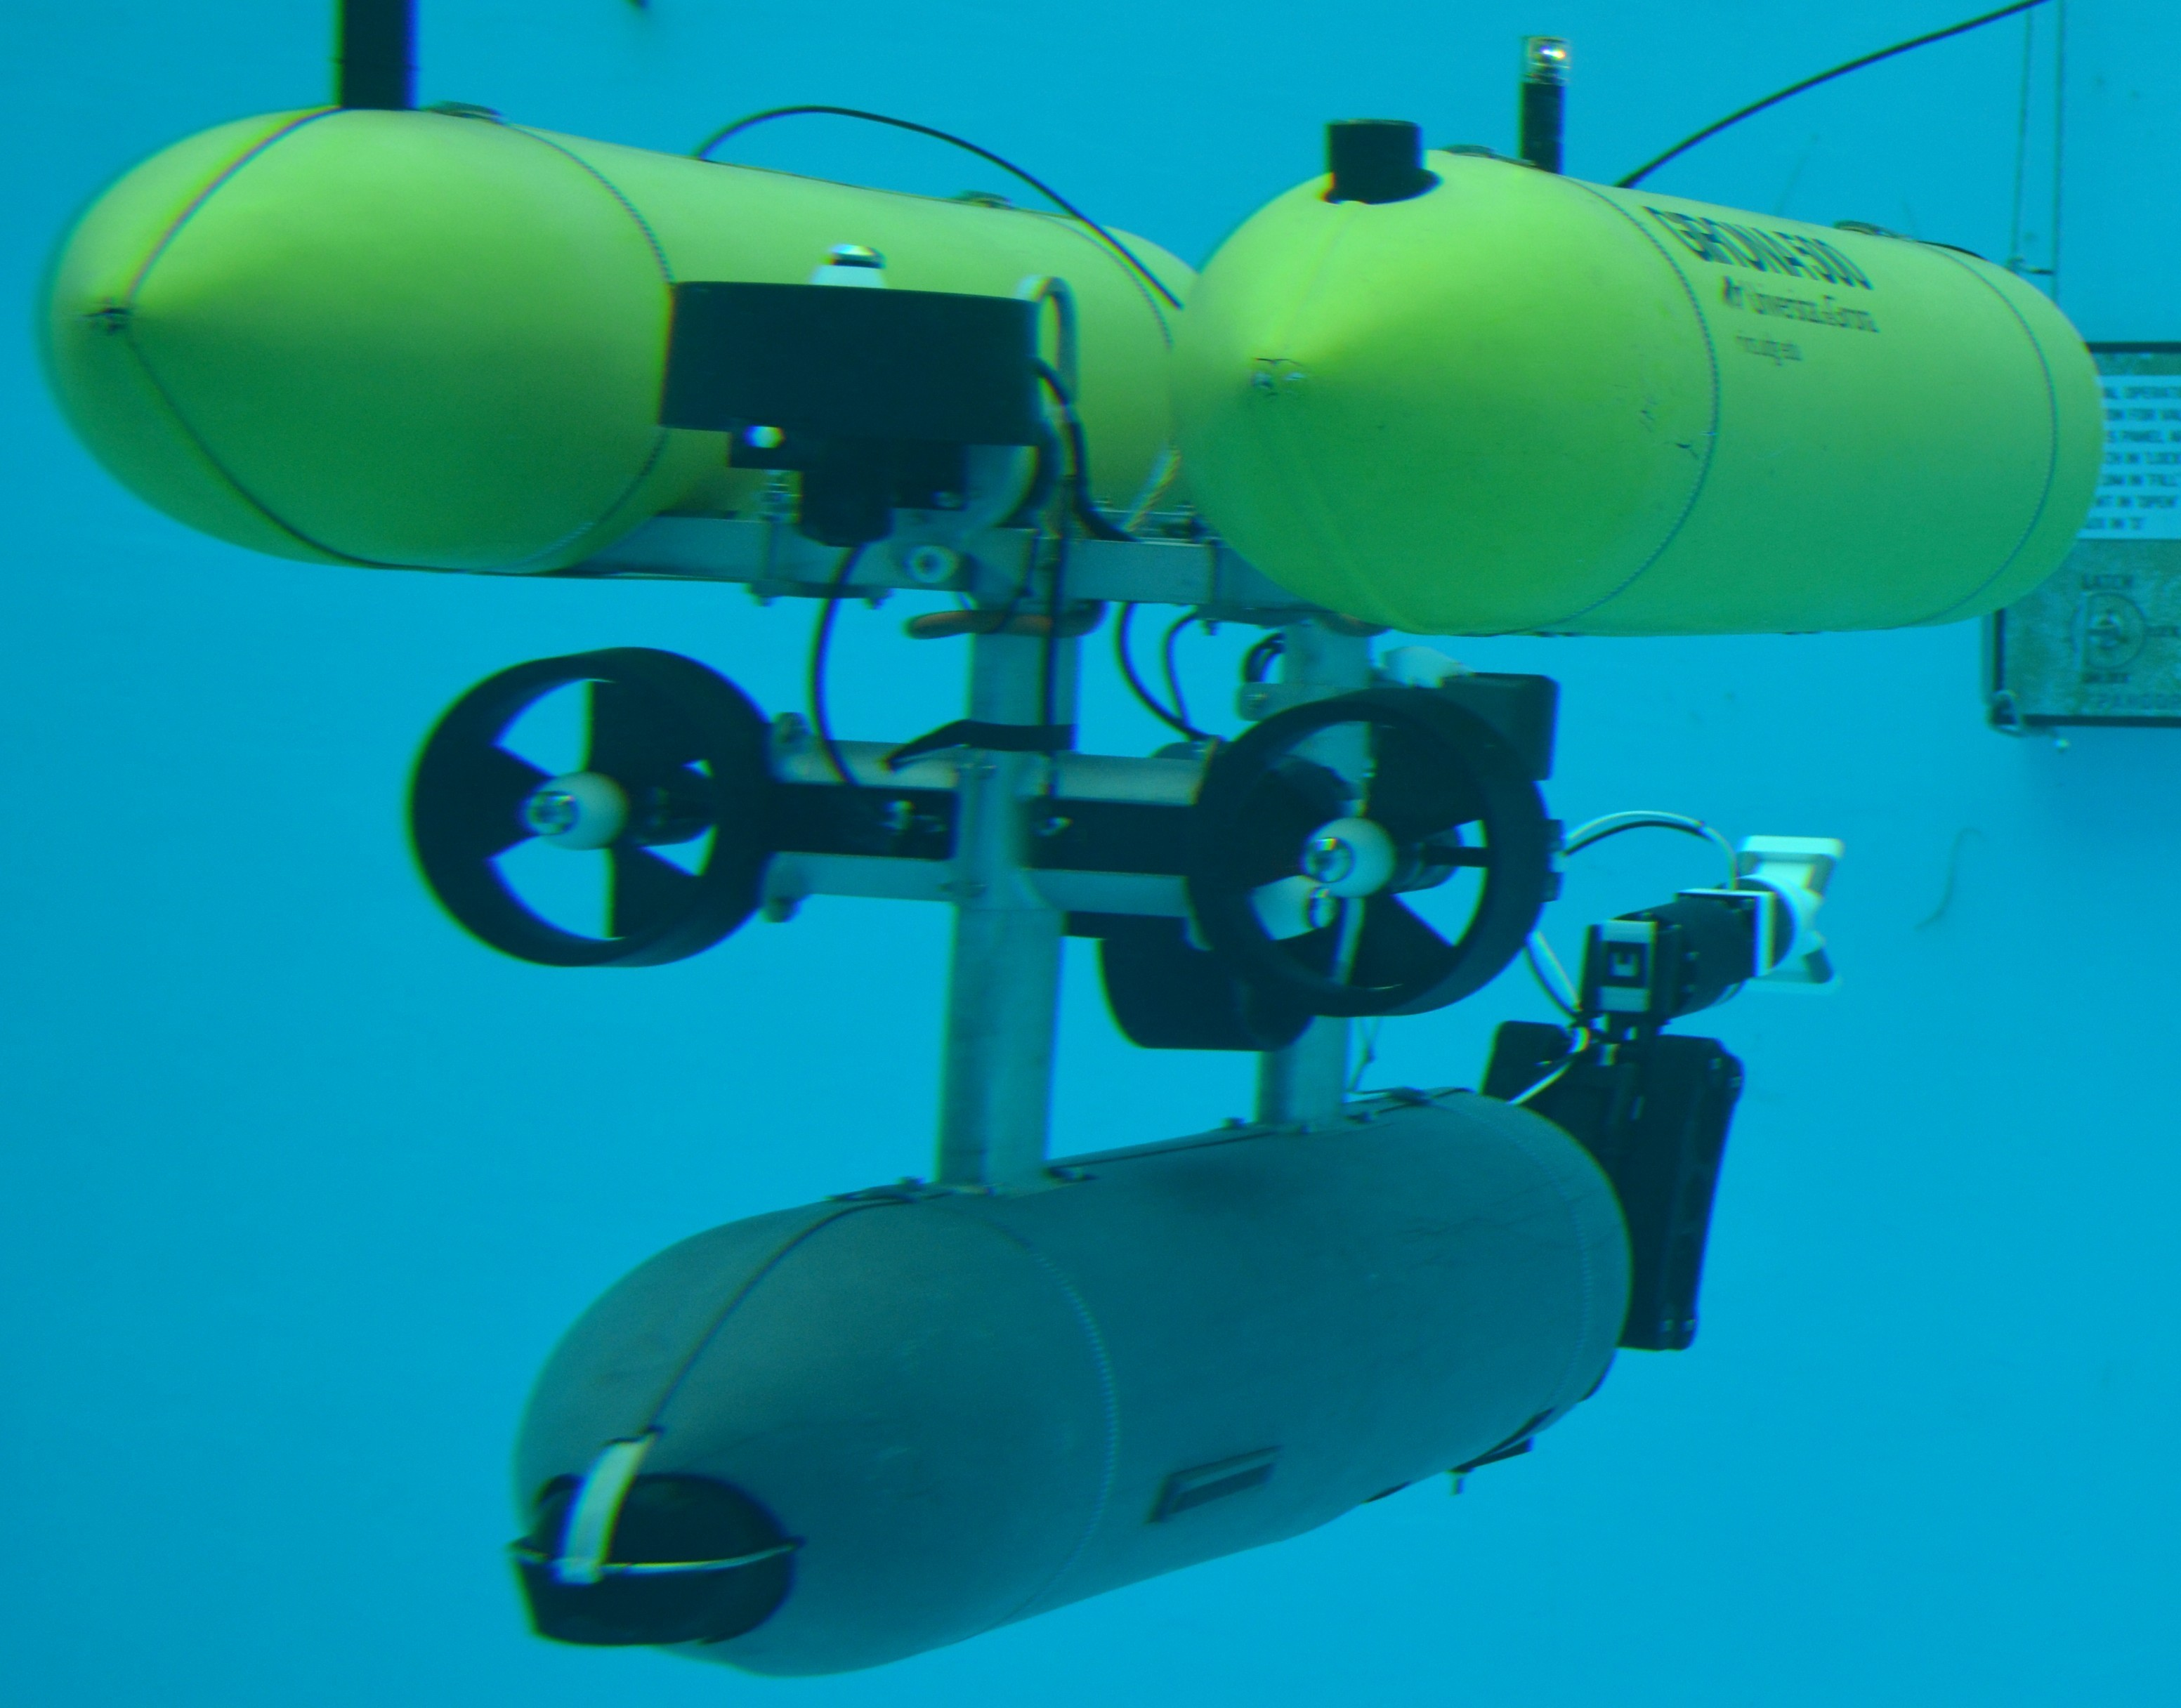
\includegraphics[scale=0.09]{./Resources/G500.jpg}
 	\caption{Fotografia do veículo submarino autônomo Girona 500}
 	\label{G500}
\end{figure}


%-----------------------------------------------------------------------------------------------------------------------------------------------------------------------------------------------
\section{OpenCV}
\textit{Open Source Computer Vision Library} (OpenCV) é uma biblioteca de código aberto, a qual reúne diversos algoritmos relacionados a visão computacional. O OpenCV foi criado pelo centro de pesquisa da \textit{Intel}, e atualmente é mantido pelo time de pesquisadores da companhia \textit{Itseez} \cite{ItseezOpenCVinfo}. A biblioteca é estruturada em diferentes módulos, os quais agrupam os algoritmos relacionados a tópicos como processamento de imagem, estimativa de movimento, correspondência estéreo, extratores de características, criação de interfaces de usuário e aceleração em \textit{hardware}. O OpenCV foi criado com a intensão de ser multiplataforma, por conta disso, em sua maior parte, foi escrito em linguagem C/C++, o que o torna facilmente portável para diversas plataformas como Windows, Linux, Android, MacOS, iOS, dentre outros. Recentemente, módulos dando suporte à CUDA (seção \ref{cuda}) e OpenGL foram incorporados à biblioteca expandindo ainda mais o número de aplicações possíveis \cite{ItseezOpenCVPlatforms}. 


%-----------------------------------------------------------------------------------------------------------------------------------------------------------------------------------------------
\section{Linux Embarcado}

Linux é um sistema operacional de código-aberto que é amplamente utilizado, cujo \textit{Kernel}, originalmente escrito por Linus Torvalds, pode suportar diversos designs de sistemas podendo ser um computador pessoal, um supercomputador ou \textit{cluster}, ou até mesmo sistemas \textit{System-on-Chip} (SoC). Este sistema é capaz de suportar diversas arquiteturas de processadores como x86{\_}64, PowerPC, ARM, MIPS, StrongARM, XScale, dentre outras \cite{Wang2011}.

A popularização do termo Linux fez com que atualmente exista uma certa confusão sobre a distinção de um \textit{Kernel} de um sistema operacional e do sistema operacional propriamente dito. A maior razão desta confusão é a interpretação errônea de termo Linux ao assumir que este é um sistema operacional. Na realidade, Linux é o \textit{kernel}, ou núcleo, do sistema operacional que, por sua vez, é simplificadamente composto pelo \textit{kernel} e o sistema de arquivos, constituindo assim uma distribuição. Atualmente, existe uma variedade de distribuições desenvolvidas pela comunidade, visto a facilidade para customizar seus módulos, pacotes, sistemas de arquivo e servidores gráficos. 

Estes sistemas também podem ser incorporadas à sistemas embarcados, também chamados de sistemas embutidos, são sistemas controlados por microprocessadores que podem ser encapsulados para realização de tarefas com dedição exclusiva para o sistema em questão. Estes sistemas são computadores totalmente especializados, diferindo de computadores de propósito geral e comumente apresentam certas restrições de dimensão, condições de operação, ou limitações de recursos computacionais (menor pode de processamento, menor capacidade de armazenamento).

Com relação à aplicação em sistemas embarcados, devido à versatilidade de sistemas baseados em Linux logo tornaram-se peças-chave para o desenvolvimento destes sistemas. Consequentemente, diversas distribuições de Linux começaram a surgir, os chamados \textit{Embedded Linux}, que apresentavam menores requisitos de sistemas, devido à remoção de módulos que não são utilizados em determinados sistemas ou à otimização desses módulos para aquela atividade específica \cite{Yaghmour2008}.

%-----------------------------------------------------------------------------------------------------------------------------------------------------------------------------------------------
\section{Aceleração em Hardware - CUDA}
\label{cuda}

\textit{Compute Unified Device Architecture} (CUDA) é uma tecnologia desenvolvida pela NVIDIA e em sua essência é uma plataforma de computação paralela de propósito geral, cujo objetivo é tirar proveito das unidades de processamento gráfico (GPU), assim, acelerando consideravelmente a execução de algoritmos computacionais complexos ao comparar-se com o desempenho em CPU. Como ilustrado pela figura \ref{cpu_gpu}, ao contrário das CPUs, as GPUs apresentam um número maior de ALUs (\textit{Arithmetic Logic Units}), as quais facilitam o processamento de dados ao permitir a paralelização das operações aritméticas.

Atualmente, a maioria das placas de vídeo da NVIDIA contam com essa tecnologia, por conta disso os pesquisadores e desenvolvedores de software estão voltando suas pesquisas para o desenvolvimento e otimização de algoritmos que possam explorar todo o poder de processamento destes dispositivos. Alguns exemplos de aplicações são identificação de placas ocultas em artérias, análise do fluxo de tráfego aéreo \cite{Monish2011} e visualização de moléculas \cite{Stone2015}.

\begin{figure}[H]
 	\centering
 	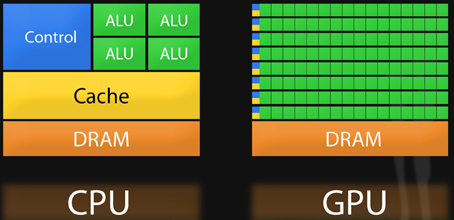
\includegraphics[scale=0.85]{./Resources/cpu_gpu.jpg}
 	\caption{Comparação entre as arquiteturas de CPU e GPU. Imagem Retirada de \cite{CUDAPython}.}
 	\label{cpu_gpu}
\end{figure}


Historicamente, a implementação de algoritmos em GPU mostrou-se bastante obscura, visto que sua programação era bastante atrelada ao hardware a ser utilizado, mesmo com linguagens de programação gráfica como o OpenGL. Em 2003, um grupo de pesquisadores de Stanford, apresentou o primeiro compilador, Brook, que facilitaria a implementação de software, visto que permitia lidar de uma maneira mais maleável o fluxo de dados, podendo principalmente paralelizá-los. Em 2006, a NVIDIA juntamente com Ian Buck, criador do Brook, desenvolveu uma plataforma (CUDA) mais intuitiva e que permitisse a utilização de uma linguagem de alto nível e tornasse a GPU em um processador de propósito geral (GPGPU) \cite{NVIDIA}.

\chapter{Materiais e Métodos}
\label{Materiais}

% Materiais e Métodos: descrição clara dos procedimentos e dos materiais adotados para o desenvolvimento do trabalho (sem resultados) incluindo sua adequação ao trabalho.
% Tem-se que responder às perguntas:
% 1) Está com um tamanho adequado (proporcional) à monografia?
% 2) Há informação suficiente e clara sobre os materiais e sobre os métodos adotados?
% Não há necessidade de reproduzir (copiar) as obras que embasam o trabalho e sim colocar o suficiente para o entendimento do trabalho e citar as referências.

Nesta seção, serão apresentados os equipamentos necessários e métodos utilizados para o desenvolvimento do projeto. No caso dos equipamentos, serão apresentados todas as especificações técnicas e sua importância para o trabalho. Na seção destinada aos métodos, os algoritmos desenvolvidos para identificação e reconhecimento de objetos serão descritos.


%-----------------------------------------------------------------------------------------------------------------------------------------------------------------------------------------------
\section{Materiais}

Com relação aos equipamentos é possível classificá-los em três grupos distintos: câmeras estéreo, unidades de processamento, e equipamentos auxiliares.


%-----------------------------------------------------------------------------------------------------------------------------------------------------------------------------------------------
\subsection{Câmeras estéreo}

As câmeras utilizadas para aplicações em visão estéreo apresentam uma série de requisitos para que seja possível desenvolver um sistema que seja facilmente embarcável e que gere um mapa de disparidades denso de qualidade, isto é, um mapa com elevado grau de detalhamento e com menor susceptibilidade a erros. Um dos requisitos que este trabalho exige é que \textit{Stereo Rig}, estrutura na qual as câmeras são fixadas, seja o mais alinhado possível. Vale ressaltar que o espaçamento das câmeras está estritamente relacionado com o espaçamento das lentes (\textit{Baseline}). Outro requisito é que essa mesma estrutura seja coerente com o tamanho do veículo e seja leve, consequentemente, diminui-se o esforço exigido pelo veículo, por exemplo, para alçar voo no caso de quadricópteros. Outro requisito é que as câmeras apresentem uma elevada taxa de captura de quadros e que sejam sincronizados, isto é, os quadros de ambas as câmeras sejam capturados no mesmo instante. Os quadros capturados devem ser disponibilizados para a plataforma embarcada via conexão USB, \textit{FireWire}, ou algum outro tipo de conexão que permita a transmissão em tempo real.

O projeto utilizou duas câmeras estéreo. Primeiramente, utilizou-se a \textit{webcam} Minoru (veja figura \ref{minoru}), visto que apresentava preço totalmente acessível e cumpria o requisito de realizar \textit{streaming} via USB. Deste modo, tornou-se um equipamento essencial para a implementação dos métodos para encontro de correspondências entre as câmeras. A tabela \ref{minoru_tab} apresenta as especificações da \textit{webcam}.

\begin{figure}[H]
	\centering
	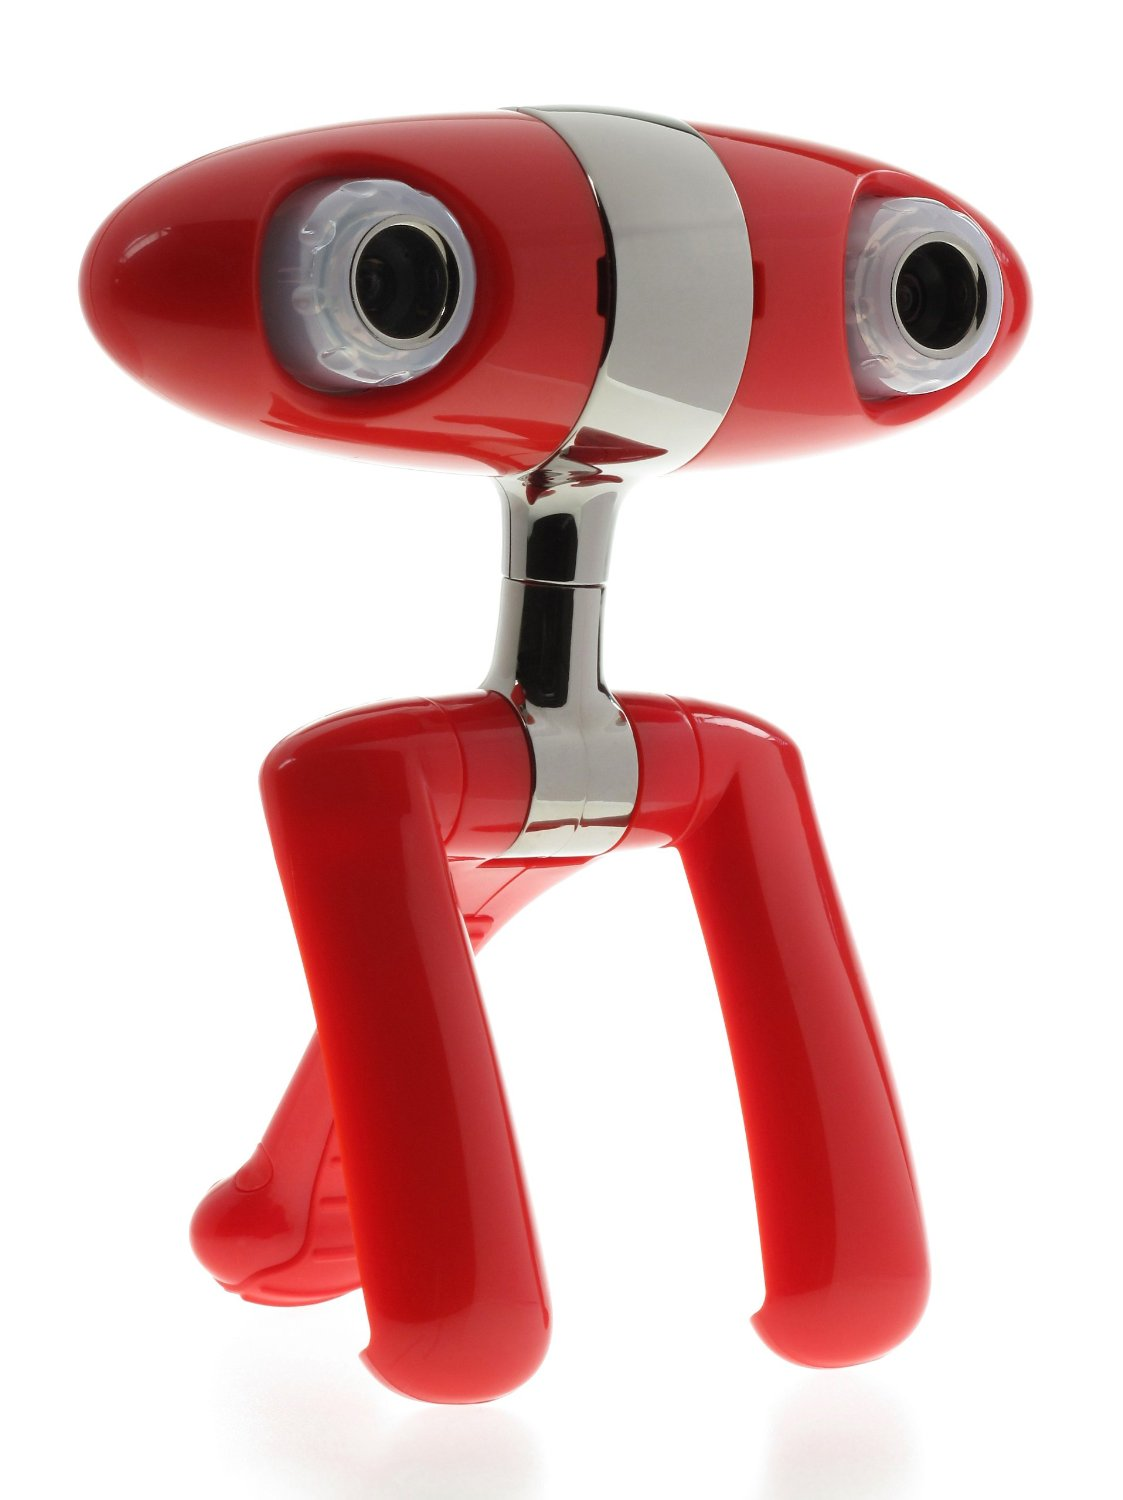
\includegraphics[scale=0.10]{./Resources/minoru.jpg}
	\caption{3D Webcam Minoru}
	\label{minoru}
\end{figure}

\begin{table}[]
\centering
\caption{Especificações - 3D Webcam Minoru}
\label{minoru_tab}
\begin{tabular}{|c|c|}
\hline
\textbf{Sensor de Imagem}      & VGA CMOS Sensor  		\\	\hline
\textbf{Resolução Máxima}      & $800x600$        		\\	\hline
\textbf{Distância entre Sensores (\textit{Baseline})} & 6 cm    \\	\hline
\textbf{Taxa de Captura}       & 30 fps             		\\	\hline
\textbf{Distância Focal}       & 10 cm até $\infty$		\\	\hline
\textbf{Campo de Visão}        & $42\degree$			\\	\hline
\textbf{Peso}		       & 249.48 g			\\	\hline
\end{tabular}
\end{table}

Atualmente, a câmera utilizada é a digital 3D W3 fabricada pela Fujifilm (veja figura \ref{fujiW3}). A primeira câmera foi substituída, pois o controlador USB não permitia que a webcam realizasse \textit{streaming} na máxima resolução. Deste modo, optou-se por uma com maior resolução e que apresentasse lentes com baixa distorção. Entretanto, essa não apresenta \textit{streaming} via USB, assim é necessário que os vídeos sejam processados \textit{offline}. Visto que o projeto se preocupa principalmente na geração do mapa de disparidades, isso não oferece nenhuma desvantagem para o desenvolvimento do trabalho. Todavia, para uma aplicação real, a câmera instalada no veículo deve apresentar esse aspecto. A tabela \ref{fujiW3_tab} apresenta as especificações da câmera em questão.

\begin{table}[]
\centering
\caption{Especificações - Câmera Digital Fujifilm FinePix Real 3D W3}
\label{fujiW3_tab}
\begin{tabular}{|c|c|}
\hline
\textbf{Sensor de Imagem}      & 10 MP CCD Sensor  		\\	\hline
\textbf{Resolução Máxima}      & $1280x720$        		\\	\hline
\textbf{Distância entre Sensores (\textit{Baseline})} & 7.5 cm  \\	\hline
\textbf{Taxa de Captura}      & 24 - 30 fps          		\\	\hline
\textbf{Distância Focal}       & 60 cm até $\infty$		\\	\hline
\textbf{Peso}       		      & 250g			\\	\hline
\end{tabular}
\end{table}

\begin{figure}[H]
	\centering
	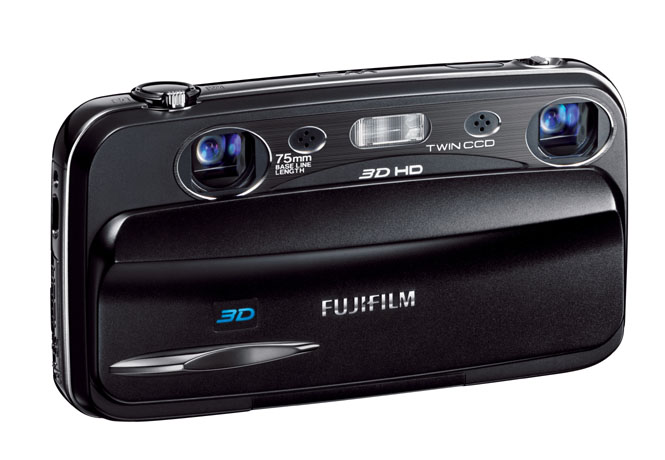
\includegraphics[scale=0.35]{./Resources/fujiW3.jpg}
	\caption{Câmera Digital Fujifilm FinePix Real 3D W3}
	\label{fujiW3}
\end{figure}


%-----------------------------------------------------------------------------------------------------------------------------------------------------------------------------------------------
\subsection{Unidades de Processamento}

Visto que este trabalho busca a implementação dos métodos estéreo em quadricópteros, tem-se como objetivo sua implementação para Linux embarcado (\textit{Embedded Linux}). Em seguida, estão apresentadas as plataformas que foram utilizadas para este propósito.


%-----------------------------------------------------------------------------------------------------------------------------------------------------------------------------------------------
\subsubsection{BeagleBone Black}

Uma das unidades de processamento utilizadas foi a plataforma aberta BeagleBone Black (BBB), ilustrada pela figura \ref{bbb}. Esta plataforma foi escolhida devido ao seu tamanho reduzido, podendo ser facilmente embarcada, isto é, é possível adaptá-la mecanicamente ao veículo. Com relação ao seu poder de processamento, ela apresenta um processador ARM Cortex-A8 operando à 1 GHz. A tabela \ref{bbb_tab} apresenta as especificações da plataforma.

\begin{table}[]
\centering
\caption{Especificações - BeagleBone Black}
\label{bbb_tab}
\begin{tabular}{|c|c|}
\hline
\textbf{Processador}           & 1GHz TI Sitara AM3359 ARM Cortex-A8			\\	\hline
\textbf{RAM}                   & 512 MB DDR3L @ 400 MHz					\\	\hline
\textbf{Armazenamento}         & 2 GB on-board eMMC, MicroSD				\\	\hline
\textbf{Sistemas Operacionais} & Angstrom (Default), Ubuntu, Android, dentre outros...	\\	\hline
\textbf{Consumo de energia}    & 210-460 mA @ 5V					\\	\hline
\textbf{Pinos de GPIO}         & 65/92 pinos						\\	\hline
\textbf{Periféricos}           & 1 USB Host, 1 Mini-USB Client, 1 10/100 Mbps Ethernet  \\	\hline                              
\end{tabular}
\end{table}

\begin{figure}[H]
	\centering
	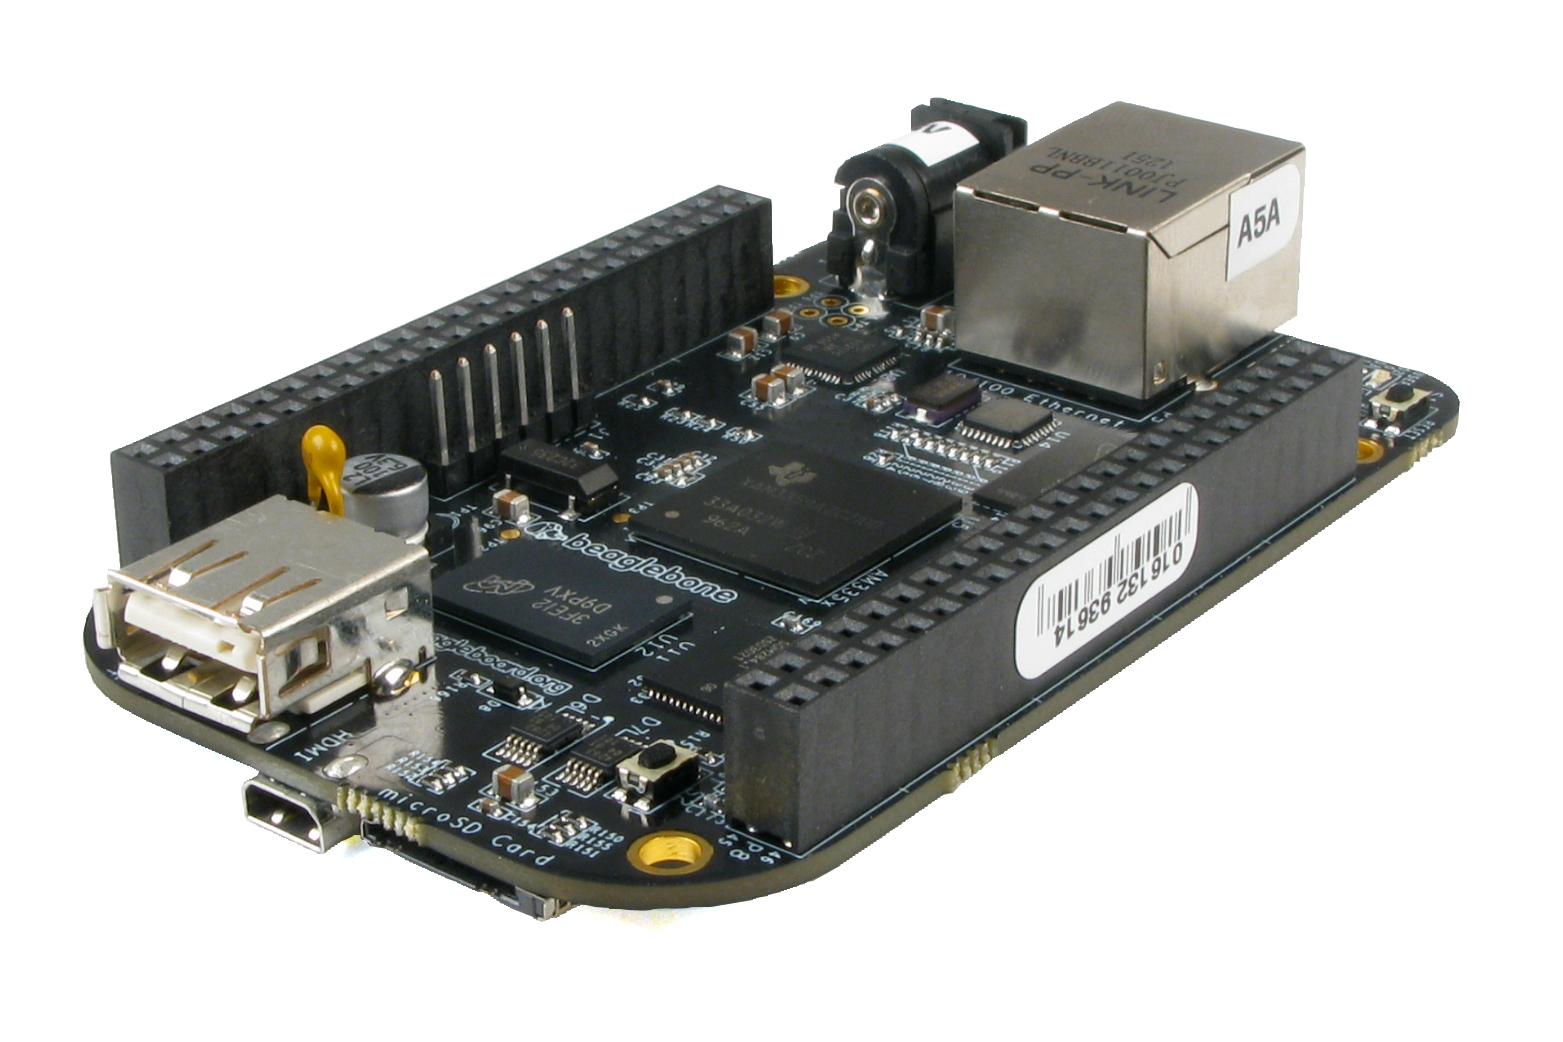
\includegraphics[scale=0.25]{./Resources/bbb.jpg}
	\caption{Plataforma de Desenvolvimento - BeagleBone Black}
	\label{bbb}
\end{figure}


%-----------------------------------------------------------------------------------------------------------------------------------------------------------------------------------------------
\subsubsection{Jetson TK1}

Outra unidade de processamento utilizada foi a plataforma \textit{Jetson TK1} produzida pela NVIDIA, ilustrada pela figura \ref{jetson_tk1}. Essa plataforma conta com um processador de 32-bits Tegra K1 baseado na tecnologia ARM Cortex-A15. O motivo pelo qual esta plataforma foi escolhida é devido ao seu poder de processamento gráfico, visto que apresenta 192 núcleos gráficos, sendo assim adequada para aplicações envolvendo processamento de imagens. A tabela \ref{jetson_tk1_tab} apresenta as especificações da plataforma. Outro fator interessante desta plataforma é que ela oferece suporte à tecnologia CUDA, a qual será discutida mais adiante.

\begin{table}[]
\centering
\caption{Especificações - \textit{Jetson TK1}}
\label{jetson_tk1_tab}
\begin{tabular}{|c|c|}
\hline
\textbf{Processador}           & NVIDIA 2.32GHz ARM quad-core Cortex-A15              \\	\hline
\textbf{Processador Gráfico}   & NVIDIA Kepler "GK20a" GPU  with 192 SM3.2 CUDA cores \\	\hline
\textbf{DRAM}                  & 2GB DDR3L 933MHz EMC x16 using 64-bit data width     \\	\hline
\textbf{Armazenamento}         & 16GB fast eMMC 4.51 (routed to SDMMC4)               \\	\hline
\textbf{Sistemas Operacionais} & Platform 64-bit Linux Ubuntu 14.04                   \\	\hline
\textbf{Consumo de energia}    & 0.6W to 3W @ 12 V                                    \\	\hline
\textbf{Pinos de GPIO}         & 7 x GPIO pins (1.8V)                                 \\	\hline
\textbf{Periféricos}           & USB, mini-PCIe, SATA, SD-card, HDMI, audio           \\	\hline
\end{tabular}
\end{table}

\begin{figure}[H]
	\centering
	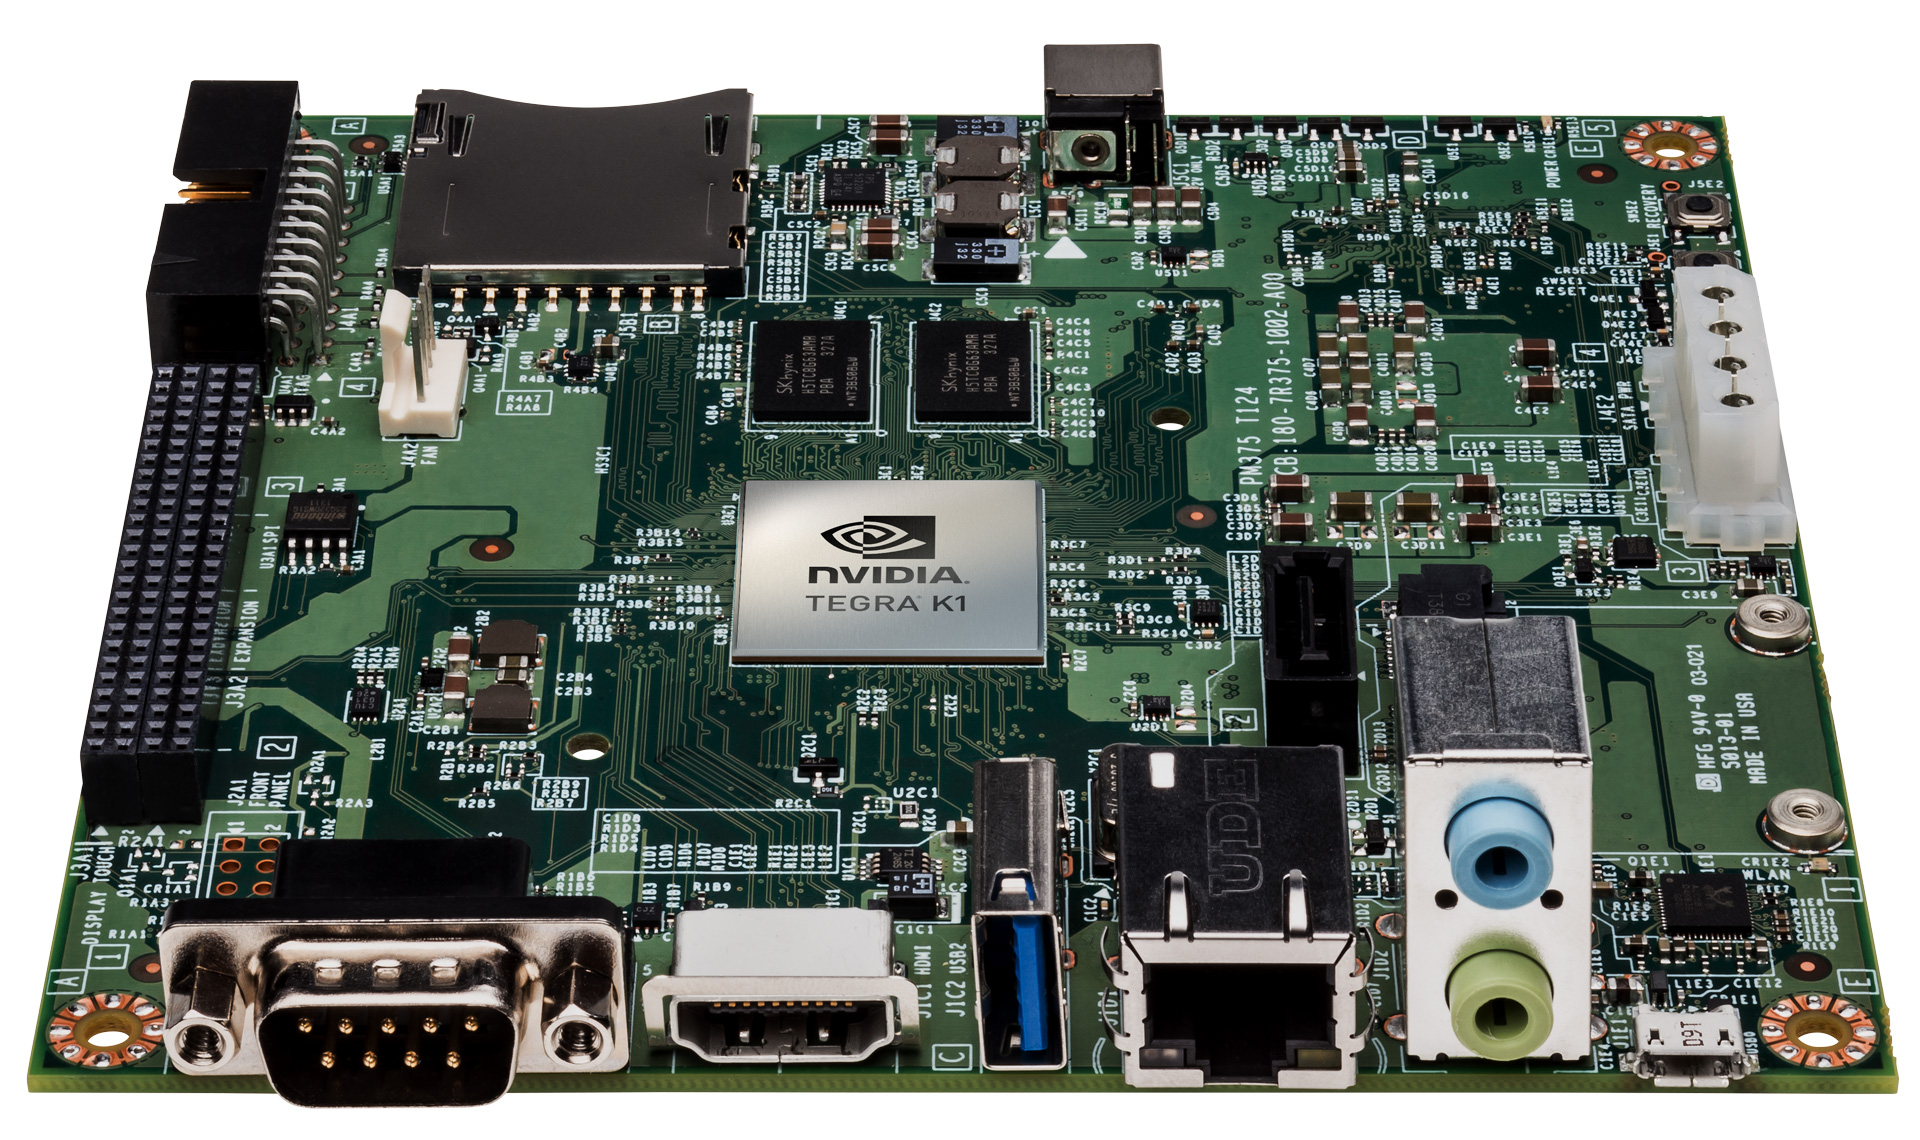
\includegraphics[scale=0.10]{./Resources/jetson_tk1.jpg}
	\caption{Plataforma de Desenvolvimento - \textit{Jetson TK1}}
	\label{jetson_tk1}
\end{figure}


%-----------------------------------------------------------------------------------------------------------------------------------------------------------------------------------------------
\subsubsection{Notebook Asus Q550LF}

Também foi utilizado um \textit{Notebook} Asus Q550LF, ele foi utilizada para o desenvolvimento de todos os programas contidos neste trabalho e para estudo de desempenho comparativo com as plataformas embarcadas. A interface desenvolvida, \textit{StereoVisionGUI}, foi desenvolvida para ser executada nesta máquina e em computadores com arquitetura x86 e x64. As especificações desta plataforma estão apresentadas pela tabela \ref{asusQ550LF}.

\begin{table}[]
\centering
\caption{Especificações - Asus Q550LF}
\label{asusQ550LF}
\begin{tabular}{|c|c|}
\hline
\multicolumn{2}{|c|}{\textbf{Especificações CPU}}                                                   \\ \hline
\textbf{CPU}             & Intel Core i7 (4th Gen) 4500U / 1.8~3.0 GHz                              \\ \hline
\textbf{Number of Cores} & Dual-Core                                                                \\ \hline
\textbf{Memory}          & DDR3 SDRAM 8 GB                                                          \\ \hline
\multicolumn{2}{|c|}{\textbf{Especificações de GPU}}                                                  \\ \hline
\textbf{Chipset}         & NVIDIA                                                                   \\ \hline
\textbf{Architecture}    & Kepler                                                                   \\ \hline
\textbf{GPU}             & GK107 384 @ 837 MHz                                                      \\ \hline
\textbf{Memory}          & DDR3 - 2048 MB - 128 Bit @ 1800 MHz                                      \\ \hline
\textbf{CUDA Cores}      & 384 Cores                                                                \\ \hline
\textbf{Features}        & Optimus, GPU Boost 2.0, PhysX, Verde Drivers, CUDA, 3D Vision, 3DTV Play \\ \hline
\end{tabular}
\end{table}


%-----------------------------------------------------------------------------------------------------------------------------------------------------------------------------------------------
\subsection{Equipamentos auxiliares}

Nesta seção, estão apresentados os equipamentos auxiliares para o desenvolvimento do trabalho. 

Os métodos para a identificação de correspondências entre as câmeras requerem que as imagens estejam calibradas e retificadas. Por conta disso, utiliza-se o padrão de calibração de dimensão 7x10, apresentado na figura \ref{calibration_pattern}, para este propósito. Deste modo, é possível caracterizar as distorções das lentes, parâmetros intrínsecos, e o posicionamento de uma das câmeras com relação a outra, parâmetros extrínsecos.  

\begin{figure}[H]
	\centering
	
\includegraphics[scale=0.10]{./Resources/calibration_pattern.png}
	\caption{Padrão de Calibração}
	\label{calibration_pattern}
\end{figure}

A motivação deste trabalho é a sua utilização em veículos aéreos. Por conta disso, é indispensável que se tenha algum desses veículos. O trabalho conta com a utilização de um quadricóptero produzido pela 3DR, porém este apresenta modificações visando o seu desenvolvimento para navegação autônoma. Deste modo, tem-se a adição de \textit{propellers guards}, objetivando o aumento da segurança do veículo e das pessoas que o operam. Além disso, o \textit{drone} conta com suportes para a câmera estéreo e para a plataforma embarcada. Como pode ser observado na figura \ref{quad_camera_support}, todas as peças foram produzidas utilizando impressora 3D.

\begin{figure}[H]
	\centering
	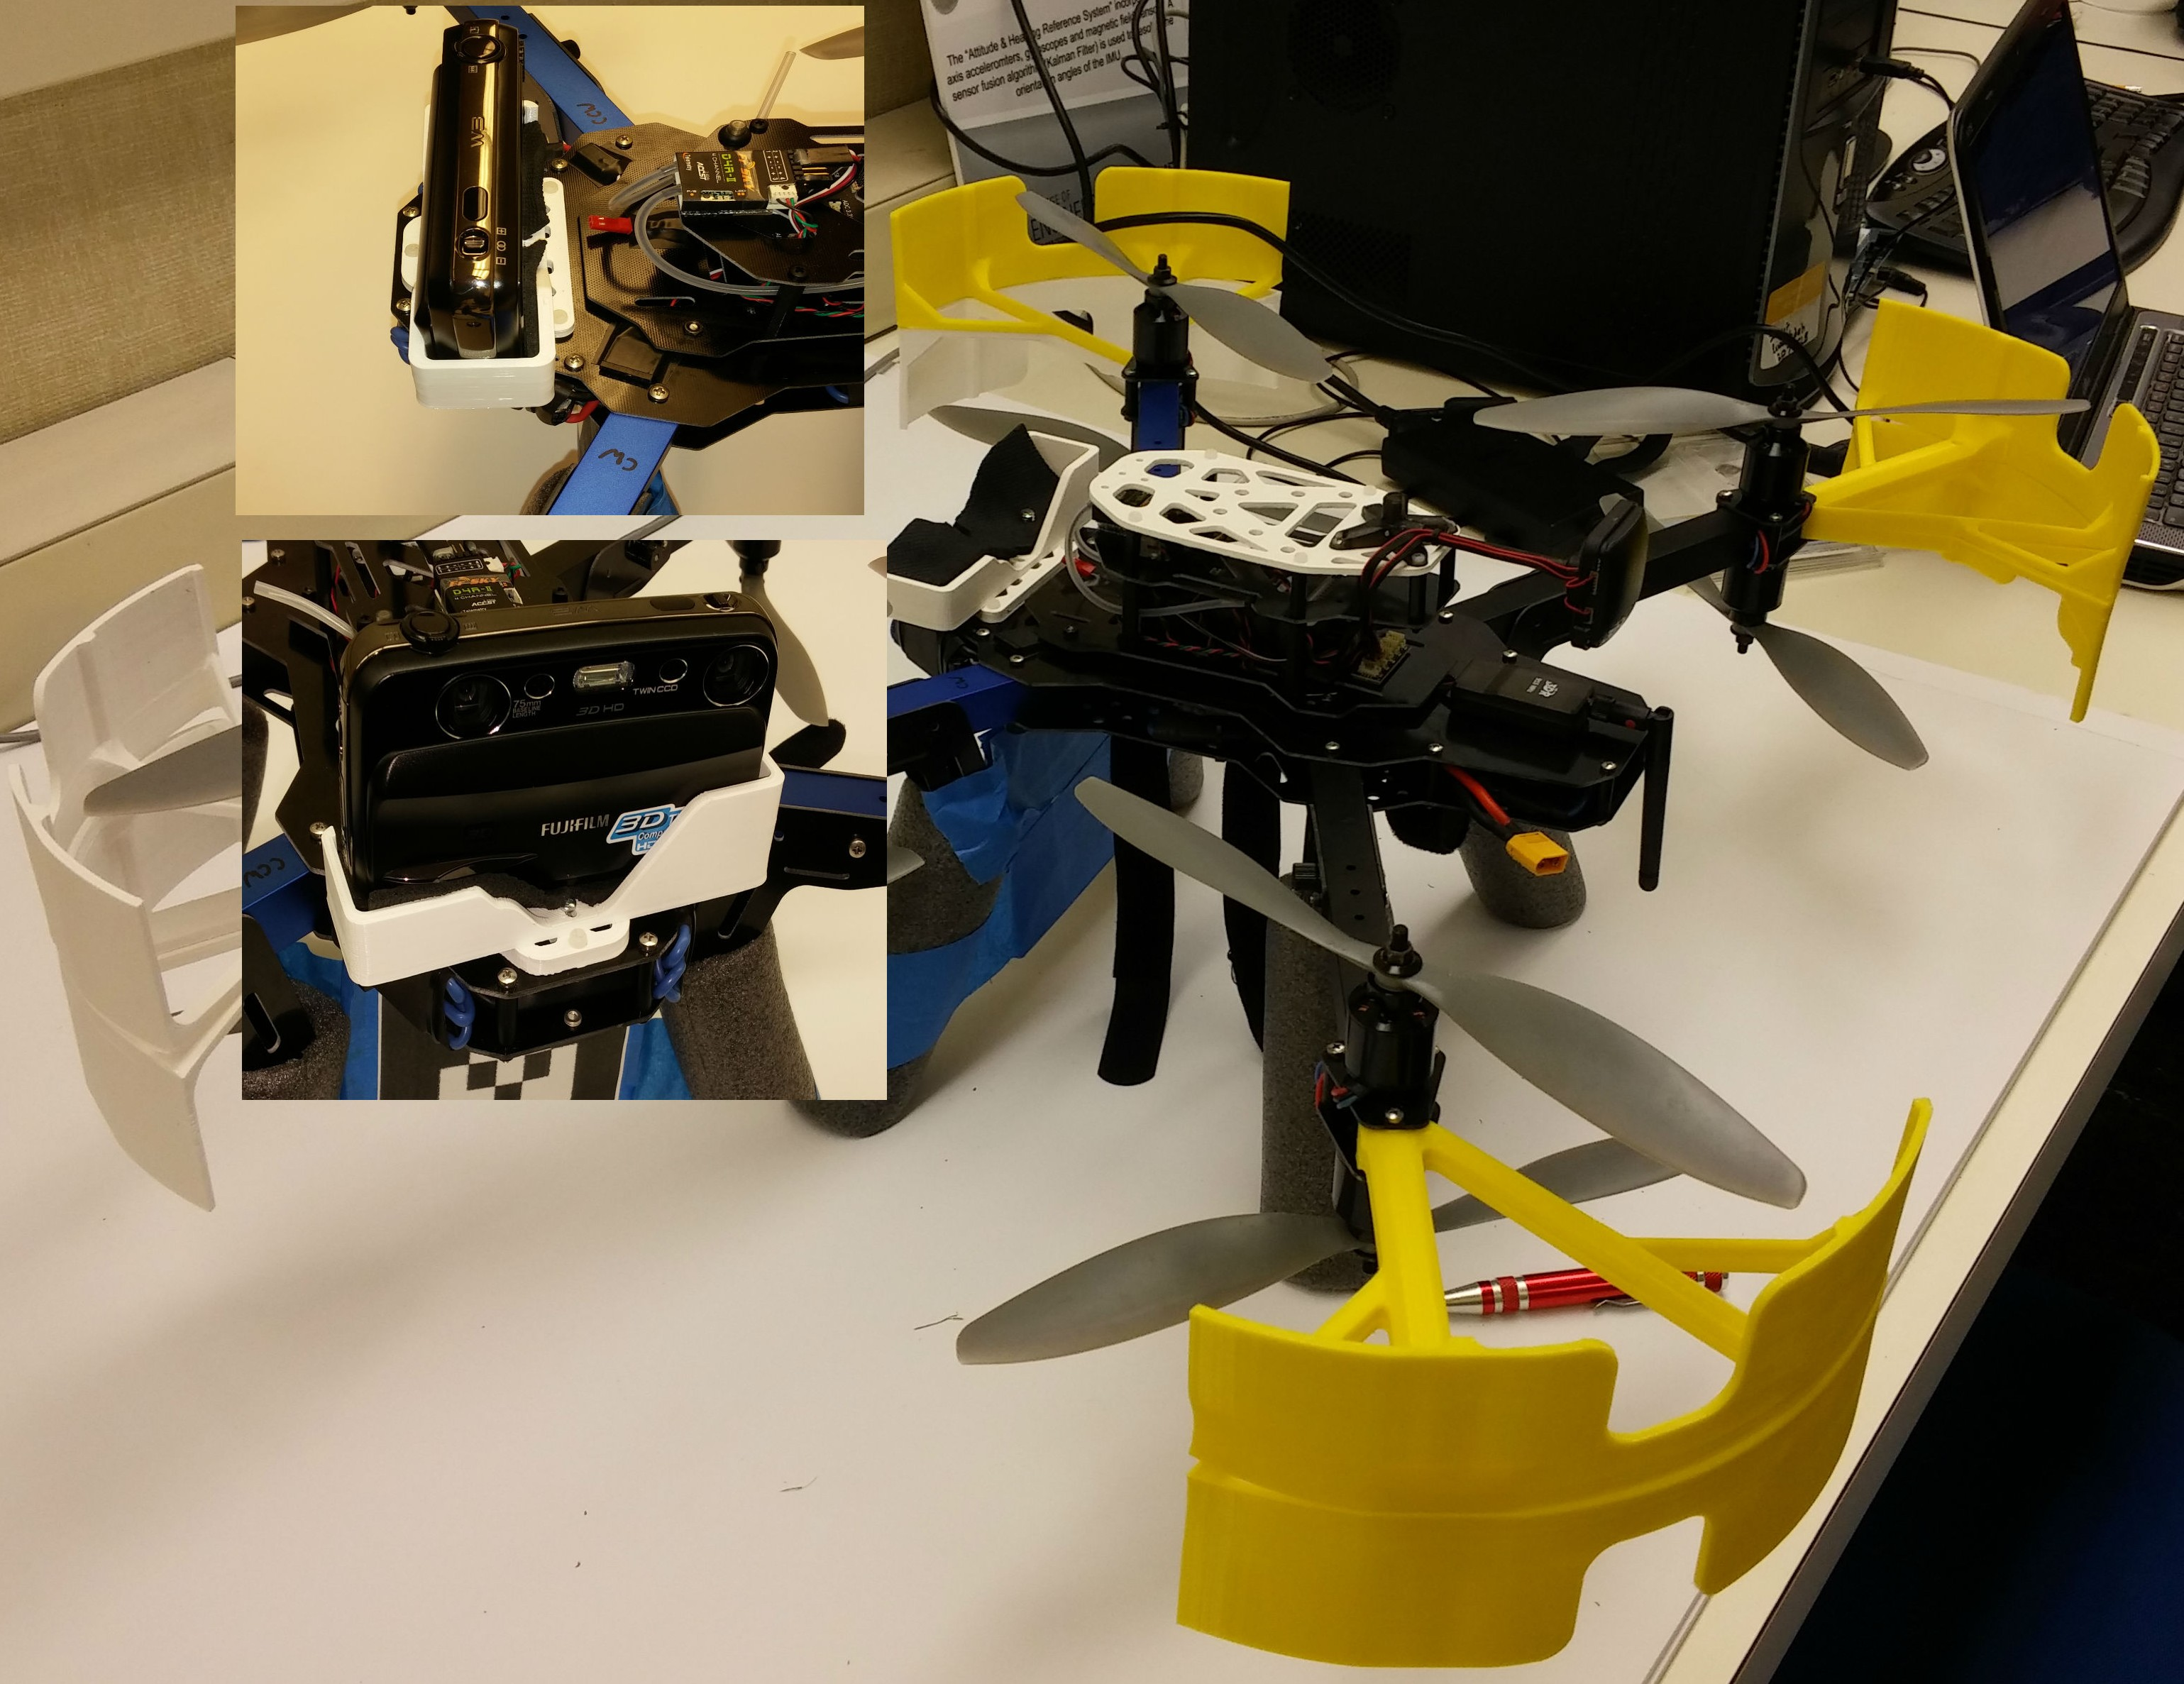
\includegraphics[scale=0.10]{./Resources/quad_camera_support.jpg}
	\caption{Quadricóptero 3DR X8 com suporte para a Câmera 3D}
	\label{quad_camera_support}
\end{figure}


%-----------------------------------------------------------------------------------------------------------------------------------------------------------------------------------------------
\section{Métodos}

Nesta seção, serão apresentados os cenários e os procedimentos utilizados na implementação dos métodos estéreo apresentados.


%-----------------------------------------------------------------------------------------------------------------------------------------------------------------------------------------------
\subsection{Cenários}
\label{scenes}

O pós-processamento do mapa de disparidades foi voltado para a identificação e detecção de obstáculos. Deste modo, os seguintes cenários propõem uma série de adversidades, as quais o algoritmo implementado tenta contorná-las. Propôs-se que ele deve ser flexível a variações na luminosidade, capaz de detectar obstáculos estáticos e móveis, e ser imune a vibrações. Deste modo, dois cenários em ambiente confinado e um em ambiente aberto foram analisados. Deseja-se a navegação autônoma ocorra até mesmo em casos que o sinal do Sistema de Posicionamento Global (GPS) seja perdido, por conta disso escolheu-se a utilização dos ambientes confinados. O ambiente externo foi escolhido devido a quantidade de fatores externos que poderiam atrapalhar a detecção de obstáculos. O tratamento destes percalços torna o programa ainda mais robusto.


%-----------------------------------------------------------------------------------------------------------------------------------------------------------------------------------------------
\subsubsection{Cenário 1}

O cenário da figura \ref{thumb_video10_l} foi utilizado para estudo das condições de ambiente externo, o qual está sujeito grandes variações de luminosidade e um número menor de movimentos, o que permite uma análise de alcances maiores. O principal  obstáculo deste cenário é uma árvore. 


%-----------------------------------------------------------------------------------------------------------------------------------------------------------------------------------------------
\subsubsection{Cenário 2}

O cenário da figura \ref{thumb_video12_l} foi utilizado para estudo das condições de ambiente interno, o qual também apresenta certa variação de luminosidade, porém apresenta um número maior de movimentos, permitindo uma análise de objetos estáticos à curta e média distância. Os principais obstáculos deste cenário são uma mesa, uma cadeira e duas estantes.


%-----------------------------------------------------------------------------------------------------------------------------------------------------------------------------------------------
\subsubsection{Cenário 3}

O cenário da figura \ref{thumb_video15} foi utilizado para estudo das condições de ambiente interno, o qual é semelhante ao cenário anterior com relação à luminosidade e o alcance analisado. A cena difere apenas na inserção de uma outra aeronave, a qual realiza o papel de um obstáculo móvel. Os principais obstáculos deste cenário é uma bancada e um outro quadricóptero no campo de visão do veículo pilotado.


%-----------------------------------------------------------------------------------------------------------------------------------------------------------------------------------------------
% Figuras
\begin{figure}[H]
	\centering
	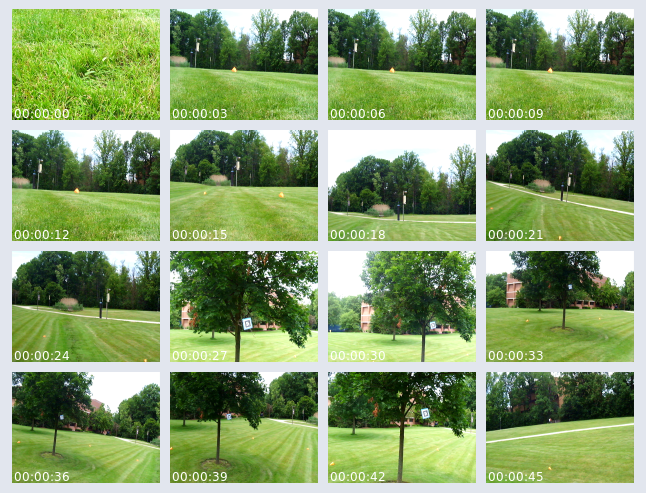
\includegraphics[scale=0.55]{./Resources/thumbs/thumb_video10_l.png}
	\caption{Cenário 1 - Ambiente Externo - Árvore}
	\label{thumb_video10_l}
\end{figure}

\begin{figure}[H]
	\centering
	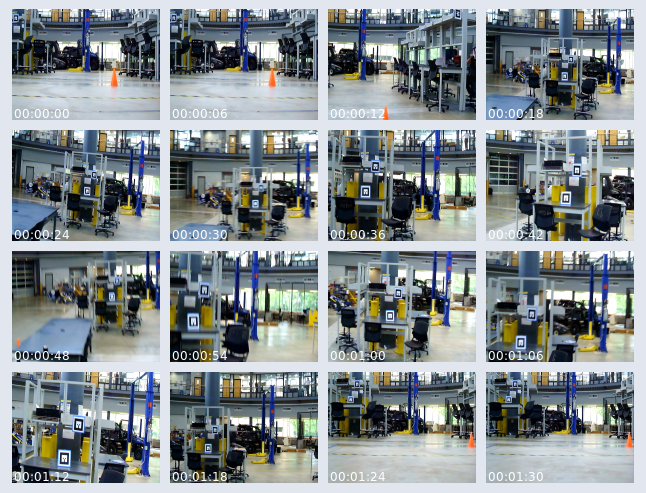
\includegraphics[scale=0.55]{./Resources/thumbs/thumb_video12_l.png}
	\caption{Cenário 2 - Ambiente Interno - Mesa/Cadeira/Estantes}
	\label{thumb_video12_l}
\end{figure}

\begin{figure}[H]
	\centering
	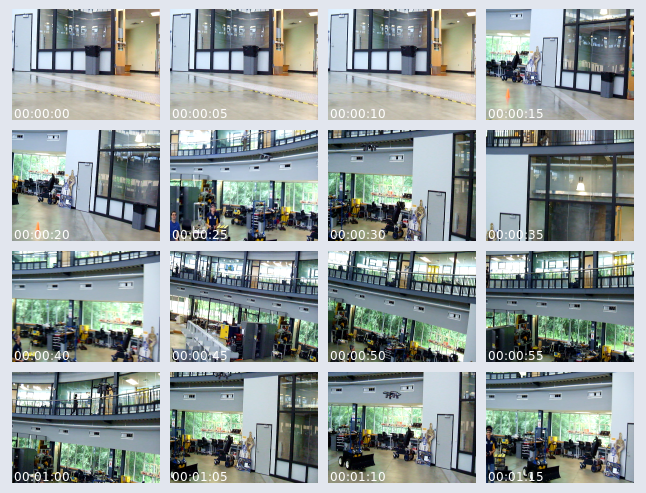
\includegraphics[scale=0.55]{./Resources/thumbs/thumb_video15.png}
	\caption{Cenário 3 - Bancada/Quadricóptero}
	\label{thumb_video15}
\end{figure}


%-----------------------------------------------------------------------------------------------------------------------------------------------------------------------------------------------
\subsection{Calibração}
O processo de calibração pode ser realizado de duas maneiras diferentes. 

O primeiro método é utilizando a rotina disponibilizada pelo OpenCV \cite{OpenCVCalibrationTutorial}, no qual algumas informações relevantes, como o tipo do padrão utilizado, o tamanho do padrão e o número de quadros, precisam ser informadas ao executá-la. Este método dispensa um conjunto de imagens de entrada para o processo de calibração, pois o próprio, automaticamente, se encarrega de detectar o padrão de calibragem e gravar as imagens utilizadas no processo. Ao fim da execução, as imagens são analisadas e os arquivos \textit{"intrinsics.yml"} e \textit{"extrinsics.yml"} são gerados, os quais contêm as matrizes que corrigem as distorções apresentadas na seção \ref{theory_calib}.

O segundo método é utilizando o aplicativo \textit{Stereo Camera Calibrator} presente no MATLAB. Ele também gera as mesmas informações anteriores, porém permite uma análise ainda mais profunda das distorções das lentes, como o erro de reprojeção 2D de cada imagem ou por pixel. Entretanto, é necessário que um conjunto de pares de imagens seja disponibilizado para o aplicativo para que a calibração seja realizada. Além disso, o MATLAB disponibiliza gráficos que representam as distorções das ambas as lentes, assim como apresentado na imagem \ref{lenses_distortion}, e a estimativa de reconstrução da cena utilizada no processo de calibração, onde estima-se o posicionamento de cada perspectiva das imagens utilizadas com relação às câmeras, assim como ilustrado na figura \ref{stereo_calib_extrinsic}.


%-----------------------------------------------------------------------------------------------------------------------------------------------------------------------------------------------
\subsubsection{Parâmetros intrínsecos}

\begin{figure}[H]
 	\centering
 	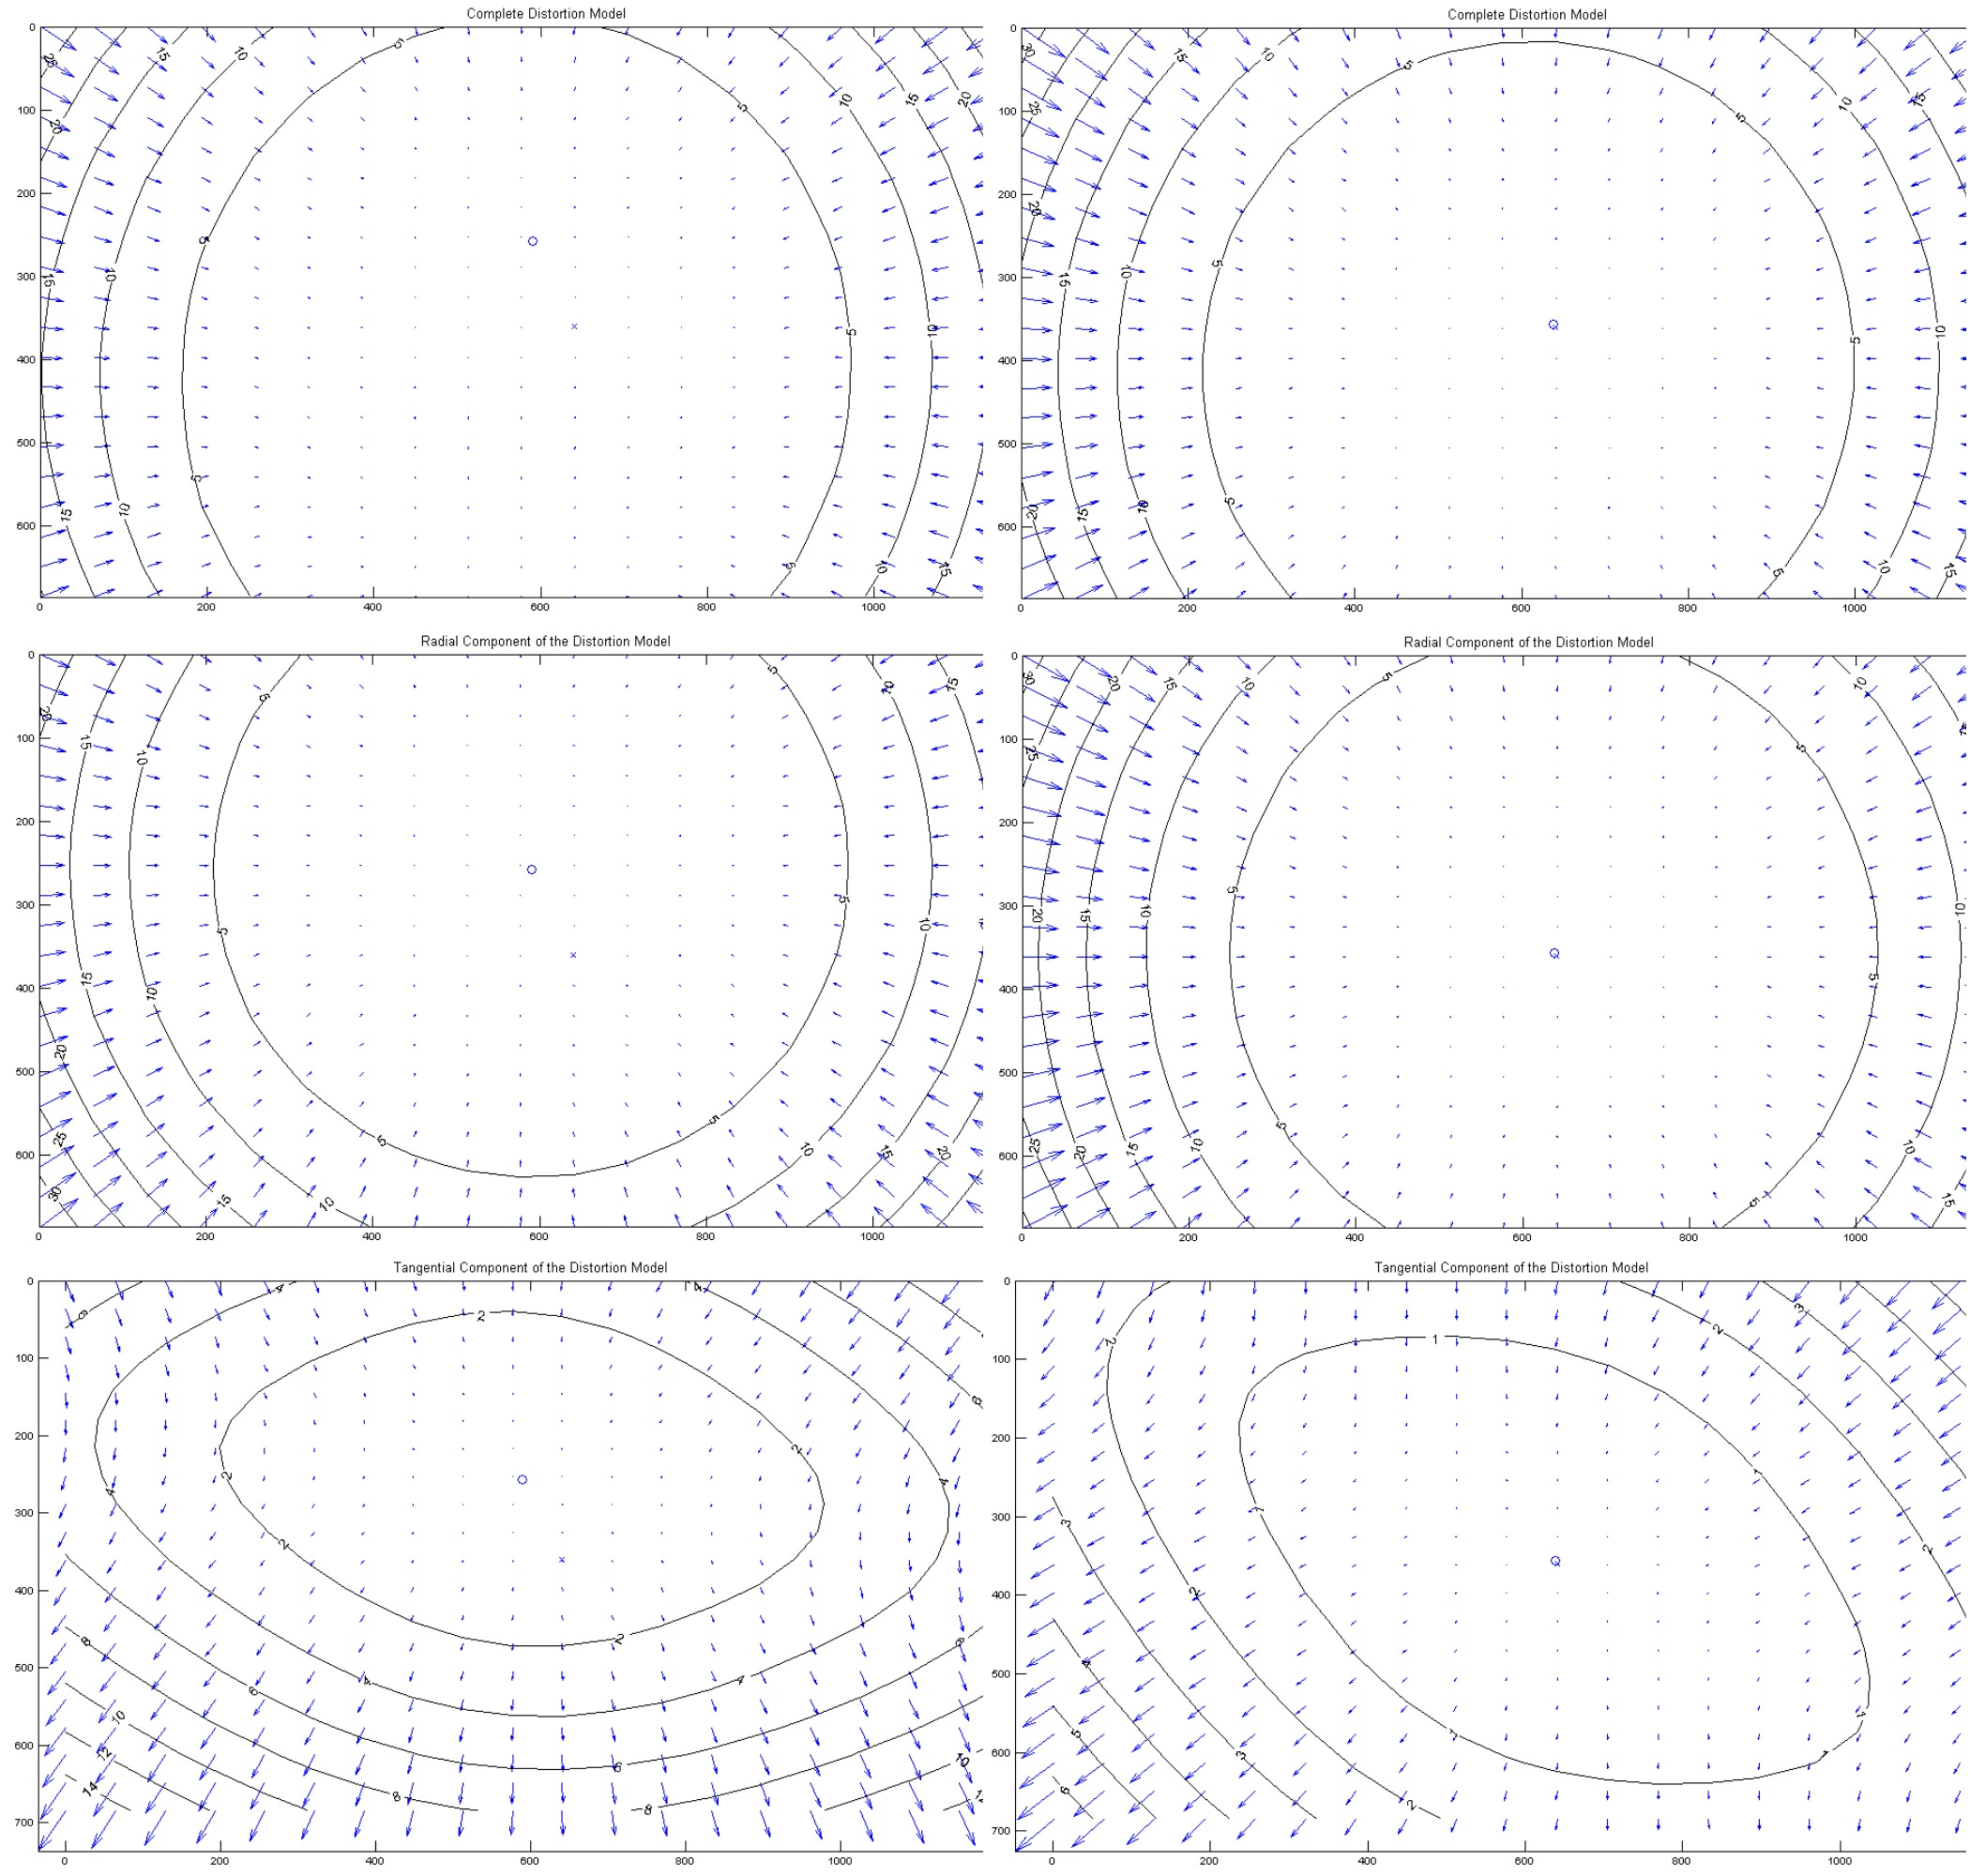
\includegraphics[scale=0.20]{./Resources/distortion/lenses_distortion.jpg}
 	\caption{Calibração estéreo dos parâmetros intrínsecos - Modelo de Distorções da câmera esquerda e direita, respectivamente. Imagem obtida utilizando \textit{Camera Calibration Toolbox for MATLAB} \cite{Bouguet1999}.}
 	\label{lenses_distortion}
\end{figure}


%-----------------------------------------------------------------------------------------------------------------------------------------------------------------------------------------------
\subsubsection{Parâmetros extrínsecos}

\begin{figure}[H]
 	\centering
 	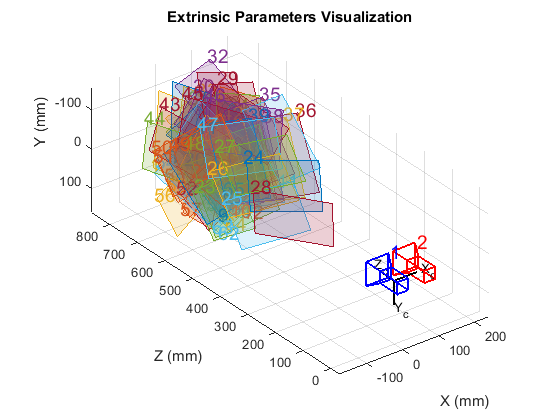
\includegraphics[scale=0.70]{./Resources/stereo_calib_extrinsic.png}
 	\caption{Calibração estéreo dos parâmetros extrínsecos - Estimativa do posicionamento da câmera direita$^2$ em relação à câmera esquerda$^1$. Imagem obtida utilizando o aplicativo \textit{Stereo Calibration App} do MATLAB \cite{MatlabStereoApp}.}
 	\label{stereo_calib_extrinsic}
\end{figure}

%-----------------------------------------------------------------------------------------------------------------------------------------------------------------------------------------------
\subsection{Processamento de Imagem}

Nessa seção será apresentado o processamento de imagens utilizado para a identificação de obstáculos. Como pode ser visto na figura \ref{stereo_processor_steps}, todo o processo conta com seis etapas.

\textbf{Câmeras:} O primeiro passo do processo é a captura das imagens da câmera estéreo. Idealmente, as imagens devem ser capturadas ao mesmo instante e as lentes não apresentarem distorções.   

\textbf{Calibração e Retificação:} Na prática, as lentes apresentam distorção. Com base nos parâmetros obtidos após a calibração das câmeras é possível retificá-las. 

\textbf{Correspondência Estéreo:} Aplica-se os métodos para encontrar as correspondências entre as duas câmeras, gerando assim o mapa de disparidades.

\textbf{Filtragem:} Este passo, pode ser aplicado tanto nas imagens retificados ou no mapa de disparidades. Atualmente, aplica-se a operação morfológica de abertura e um filtro de mediana sobre o mapa de disparidades. 

\textbf{Limiarização por Distância:} Visto que a disparidade apresenta uma relação com a distância, aplica-se uma operação de limiarização. Deste modo, apenas os obstáculos a uma certa distância são segmentados.

\textbf{Identificação de Obstáculos:} Após o passo anterior, o objeto é identificado e sua posição é rastreada. Essa informação pode ser utilizada pelo sistema de controle da aeronave para manter distância do obstáculo identificado. Esta etapa encontra-se realçada na figura \ref{stereo_processor_steps}, pois o processo de segmentação e identificação de objetos varia conforme o tipo de obstáculo e as condições da imagem (claro, escuro, muito brilho, baixo contraste). Deste modo, uma árvore de opções surge a partir deste processo, todos com o intuito de contornar as adversidades presentes no ambiente.

\begin{figure}[H]
	\centering
	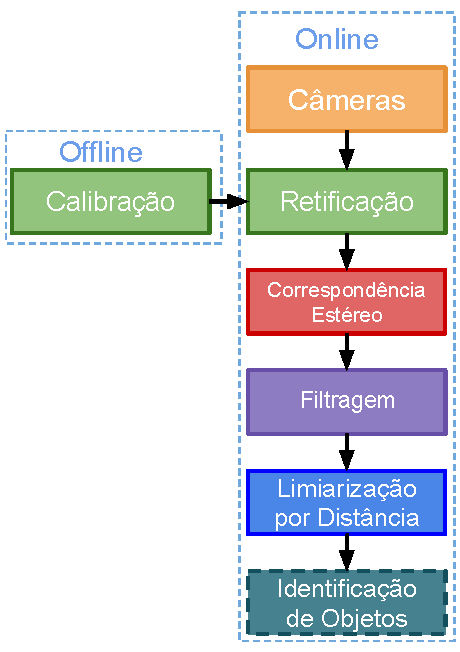
\includegraphics[scale=1.0]{./Resources/stereo_processor_steps3.pdf}
	\caption{Etapas do Processamento de Imagens}
	\label{stereo_processor_steps}
\end{figure}


%-----------------------------------------------------------------------------------------------------------------------------------------------------------------------------------------------
\subsection{Aceleração em Hardware - \textit{Hardware Acceleration} - CUDA}

Neste trabalho, utilizou-se diferentes versões desta API (\textit{Application Programming Interface}) para o desenvolvimento para \textit{Desktop} e \textit{Jetson TK1}. Neste contexto, essas versões não oferecem nenhuma alteração visível, visto que não foi desenvolvido nenhum tipo de rotina especificamente para execução em GPU. Na verdade, utilizou-se as funções disponíveis na biblioteca OpenCV, as quais opcionalmente podem ser executadas pela CPU ou GPU. A tabela \ref{cudaopencv} informa as versões do pacote de ferramentas da plataforma CUDA e da biblioteca OpenCV utilizadas. 

\begin{table}[]
\centering
\caption{Versões utilizadas de CUDA e OpenCV}
\label{cudaopencv}
\begin{tabular}{cccll}
                     & \textbf{CUDA ToolKit}	     & \textbf{OpenCV} 	       &  &  \\
\textbf{Desktop}     & 7.5                           & 3.0.0                   &  &  \\
\textbf{Jetson TK1}  & 6.5                           & 2.4.12                  &  &  \\
\multicolumn{1}{l}{} & \multicolumn{1}{l}{}          & \multicolumn{1}{l}{}    &  & 
\end{tabular}
\end{table}

\subsubsection{Desktop - Instalação e Configuração}
Abaixo, estão apresentadas as instruções necessárias para a instalação e a configuração do ambiente de desenvolvimento para que plataforma CUDA funcione corretamente \cite{FacebookCUDA}. O seguinte processo também pode ser executado para a configuração do ambiente na \textit{Jetson TK1}. Entretanto, um processo muito mais intuitivo e recomendado para essa plataforma está apresentado na seção \ref{jetsonSetupCUDA}.

\begin{enumerate}
 \item Instalando a CUDA
 
 Primeiramente, as seguintes instruções são compatíveis somente em máquinas com Ubuntu 14.04+ e com processadores gráficos da NVIDIA com capacidade de computação 3.5 ou maior. 
 \begin{enumerate}
  \item  Execute o seguinte comando:
  
\begin{lstlisting}[basicstyle=\tiny]
  $ ubuntu@ubuntu:~$ sudo apt-­get install build­-essential
\end{lstlisting}
  
Caso o usuário esteja utilizando uma máquina virtual, é necessário que os seguintes comandos sejam executados:

\begin{lstlisting}[basicstyle=\tiny]
  $ ubuntu@ubuntu:~$ sudo apt-get update
  $ ubuntu@ubuntu:~$ sudo apt-get install linux-generic
\end{lstlisting}

\item Baixe o arquivo .deb da CUDA no seguinte link: \url{https://developer.nvidia.com/cuda-downloads}, e verifique se a versão do arquivo é correspondente ao sistemas operacional utilizado. Neste trabalho, utilizou-se o Linux Ubuntu 14.04 64-bit e o arquivo condizente chamava-se "cuda-repo-ubuntu1404-7-5-local\_7.5-18\_amd64.deb" e foi possível instalá-lo recorrendo aos seguintes comandos:

\item Execute os seguintes comandos:

\begin{lstlisting}[basicstyle=\tiny]
$ ubuntu@ubuntu:~$ cd Downloads
$ ubuntu@ubuntu:~/Downloads$ sudo dpkg -i cuda-repo-ubuntu1404-7-5-local_7.5-18_amd64.deb
$ ubuntu@ubuntu:~/Downloads$ sudo apt-get update
$ ubuntu@ubuntu:~/Downloads$ sudo apt-get install cuda

\end{lstlisting}

\item Configure as variáveis do ambiente necessárias para o desenvolvimento em programação CUDA:
 
\begin{lstlisting}[basicstyle=\tiny]
$ ubuntu@ubuntu:~/Downloads$ nano ~/.bashrc

-----------------------------------------------------------------------
    Edite o arquivo /home/<user>/.bashrc e adicione o seguinte trecho:
-----------------------------------------------------------------------
# CUDA Environment Setup 
# CUDA 6.5
#export PATH=/usr/local/cuda-6.5/bin:$PATH
#export LD_LIBRARY_PATH=/usr/local/cuda-6.5/lib64:$LD_LIBRARY_PATH

# CUDA 7.5 (active)
export PATH=/usr/local/cuda-7.5/bin:$PATH
export LD_LIBRARY_PATH=/usr/local/cuda-7.5/lib64:$LD_LIBRARY_PATH

$ ubuntu@ubuntu:~/Downloads$ source ~/.bashrc
\end{lstlisting}

\item Reinicie o computador.
 \end{enumerate}

  \item Instalando do OpenCV com Suporte à CUDA \cite{Harasimowicz2015}
  \begin{enumerate}
   \item Instalando os pacotes necessários
   \begin{lstlisting}[basicstyle=\tiny]
$ ubuntu@ubuntu:~$ sudo apt-get update

$ ubuntu@ubuntu:~$ sudo apt-get install libopencv-dev build-essential checkinstall 
		   cmake pkg-config yasm libtiff4-dev libjpeg-dev libjasper-dev 
		   libavcodec-dev libavformat-dev libswscale-dev libdc1394-22-dev 
		   libxine-dev libgstreamer0.10-dev libgstreamer-plugins-base0.10-dev 
		   libv4l-dev python-dev python-numpy libtbb-dev libqt4-dev libgtk2.0-dev 
		   libfaac-dev libmp3lame-dev libopencore-amrnb-dev libopencore-amrwb-dev 
		   libtheora-dev libvorbis-dev libxvidcore-dev x264 v4l-utils
$ ubuntu@ubuntu:~$ sudo add-apt-repository ppa:jon-severinsson/ffmpeg  
$ ubuntu@ubuntu:~$ sudo apt-get update  
$ ubuntu@ubuntu:~$ sudo apt-get install ffmpeg  
$ ubuntu@ubuntu:~$ sudo apt-get install frei0r-plugins
   \end{lstlisting}

   \item Clonando o repositório do OpenCV. Neste trabalho, utilizou-se a versão 3.0.0:
   \begin{lstlisting}[basicstyle=\tiny]
$ ubuntu@ubuntu:~$ mkdir OpenCV  
$ ubuntu@ubuntu:~$ cd OpenCV
$ ubuntu@ubuntu:~/OpenCV$ git clone https://github.com/Itseez/opencv.git  
   \end{lstlisting}


   \item Instalando e realizando o \textit{build} da biblioteca OpenCV. Este passo é de extrema importância, pois é aqui que configura-se o OpenCV para dar suporte à CUDA. Certifique-se que a arquitetura de GPU configurada na \textit{flag} CUDA\_GENERATION corresponda realmente a da sua plataforma:
   \begin{lstlisting}[basicstyle=\tiny]
$ ubuntu@ubuntu:~/OpenCV$ mkdir build && cd build
$ ubuntu@ubuntu:~/OpenCV/build$ cmake -D CMAKE_BUILD_TYPE=RELEASE -D CMAKE_INSTALL_PREFIX=/usr/local 
-D WITH_TBB=ON -D WITH_V4L=ON -D INSTALL_C_EXAMPLES=ON -D INSTALL_PYTHON_EXAMPLES=ON -D BUILD_EXAMPLES=ON 
-D WITH_QT=ON -D WITH_OPENGL=ON -D ENABLE_FAST_MATH=1 -D CUDA_FAST_MATH=1 -D WITH_CUBLAS=1 -D CUDA_GENERATION=Kepler ..
$ ubuntu@ubuntu:~/OpenCV/build$ make -j4
$ ubuntu@ubuntu:~/OpenCV/build$ sudo make install
    \end{lstlisting}

   \item Configurando o \textit{LIBRARY SEARCH PATH}:
   \begin{lstlisting}[basicstyle=\tiny]
$ ubuntu@ubuntu:~/$ sudo sh -c 'echo "/usr/local/lib" > /etc/ld.so.conf.d/opencv.conf'
$ ubuntu@ubuntu:~/$ sudo ldconfig

  \end{lstlisting}

  \end{enumerate}

\end{enumerate}

%-----------------------------------------------------------------------------------------------------------------------------------------------------------------------------------------------
\subsection{Jetson TK1 - Configuração da Plataforma}
\label{jetsonSetupCUDA}

A execução das rotinas de visão estéreo com aceleração via GPU requisitam que a plataforma de desenvolvimento esteja corretamente configurada. Abaixo, encontra-se o tutorial para configurá-la para a operação desejada, isto é, basicamente, configurá-la para o correto funcionamento da CUDA e do OpenCV2. 

\begin{enumerate}
  \item Baixando o JetPack L4T
    \begin{enumerate}
      \item Clique \href{http://docs.nvidia.com/jetpack-l4t/index.html#developertools/mobile/jetpack/jetpack_l4t/2.1/jetpack_l4t_install.htm}{aqui} para ir ser redirecionado para a página do pacote de desenvolvimento Jetpack L4T. Caso o link esteja quebrado, vá até a página da NVIDIA e procure pela localização correta do pacote.  

      \item Na máquina \textit{Host} rodando Ubuntu, crie um novo diretório para armazenar os pacotes de instalação utilizando as seguintes linhas de comando.

      \begin{lstlisting}[basicstyle=\tiny]
	$ ubuntu@ubuntu:~$ mkdir flash
	$ ubuntu@ubuntu:~$ cd flash
	$ ubuntu@ubuntu:~/flash$ 
      \end{lstlisting}

      Uma ação importante que merece destaque é baixar o arquivo JetPack-\${VERSION}.run dentro do diretório criado (o caminho NÃO DEVE conter espaços).

      \item Dê permissão de execução para o arquivo baixado. 
      \begin{lstlisting}[basicstyle=\tiny]
	$ ubuntu@ubuntu:~/flash$ chmod +x JetPack-${VERSION}.run
	$ ubuntu@ubuntu:~/flash$ ./JetPack-${VERSION}.run
      \end{lstlisting}


    \end{enumerate}
  \item Instalando o JetPack L4T

    Siga as instruções no manual de usuário do kit de desenvolvimento da \textit{Jetson TK1}
    \begin{enumerate}
      \item Baixe o guia de instruções no seguinte link e clique na aba "\textit{Install Guide}". Link: \url{https://developer.nvidia.com/embedded/jetpack}
      \item Siga as instruções do instalador do Jetpack L4T.

      Uma informação que merece destaque é que o computador \textit{Host} e o dispositivo alvo (\textit{Jetson TK1}) DEVEM estar conectados à mesma rede. Isso pode ser feito conectando:
      \begin{enumerate}
	\item Máquina \textit{Host} e dispositivo alvo à mesma Intranet, no caso o dispositivo alvo tenha um endereço IP estático.
	\begin{lstlisting}[basicstyle=\tiny]
	    ----------------------------------------------------
	    Edite o /etc/network/interfaces:
	    ----------------------------------------------------    
	    auto lo
	    iface lo inet loopback
	    auto eth0
	    iface eth0 inet static
	    address 10.235.0.133
	    netmask 255.255.252.0
	    network 10.235.3.0
	    gateway 10.235.0.1
	    pre-up ifconfig eth0 hw ether 00:01:02:03:05:09
	    dns-nameservers  143.107.225.6 143.107.182.2 8.8.8.8
	 \end{lstlisting}

	 \item Máquina \textit{Host} e dispositivo alvo ao mesmo roteador. Neste caso, o dispositivo alvo DEVE ser capaz de encontrar o endereço IP por protocolo DHCP.
	 \begin{lstlisting}[basicstyle=\tiny]
	    ----------------------------------------------------
	    Edite o /etc/network/interfaces:
	    ----------------------------------------------------    
	    auto eth0
	    allow-hotplug eth0
	    iface eth0 inet dhcp
	 \end{lstlisting}
      \end{enumerate}


    \end{enumerate}
  \item Instalando o OpenCV com Módulo GPU na \textit{Jetson TK1}

  Primeiramente, deve-se baixar e instalar o pacote de ferramentas CUDA, uma vez que é necessário para OpenCV. Cabe ao usuário decidir se deseja se utilizar a biblioteca pré-compilada ou compilar a biblioteca do código-fonte. A primeira opção é a mais recomendada, visto que a biblioteca pré-compilada é a OpenCV4Tegra, uma versão otimizada em CPU e GPU do OpenCV para a \textit{Jetson TK1}. A segunda opção é recomendada caso deseja-se adicionar módulos que não estão presentes na versão OpenCV4Tetra \cite{eLinuxJetsonOpenCV}. 

\end{enumerate}

%-----------------------------------------------------------------------------------------------------------------------------------------------------------------------------------------------
% Resultados/Discussões: 
% Aqui se mostra o que o trabalho permitiu produzir, e às vezes o que pode ser comparado com outros trabalhos
% Aqui ficam claras se as propostas do trabalho são relevantes ou não, pois devem permitir a discussão do trabalho;
% Deve-se responder: Os resultados estão claros em bom número (nem muito nem pouco) que permitam avaliar realmente a proposta e o que foi produzido.
\chapter{Resultados}
\label{Resultados}

Os resultados apresentados neste capítulo estão divididos em duas partes. Os resultados da seção \ref{resultsGUI} estão inteiramente relacionados às funções fundamentais presentes na interface gráfica desenvolvida. Já na seção \ref{resultsComparison}, têm-se presente os resultados que apresentam os dados obtidos por meio dos testes de desempenho dos métodos de \textit{Stereo Matching} nas plataformas utilizadas.

%-----------------------------------------------------------------------------------------------------------------------------------------------------------------------------------------------
\section{Interface Gráfica - \textit{StereoVisionGUI}}
\label{resultsGUI}

Nesta seção, o software desenvolvido apresenta uma interface gráfica (GUI -- \textit{Graphical User Interface}) amigável, a qual facilita a visualização das imagens da câmera estéreo, 
dos mapas de disparidades, da reconstrução tridimensional e do método de processamento de imagens desenvolvido. Atualmente, o software conta com três métodos para encontrar correspondências 
estéreo (BM, SGBM e BMGPU) e com 8 opções das quais 6 delas são destinadas a visualização das seguintes perspectivas:

\begin{enumerate}
  \item Imagens retificadas das câmeras esquerda e direita
  \item Mapa de disparidades em Escala de Cinza e RGB
  \item Mapa tridimensional do ambiente reconstruído em Escala de Cinza e RGB
  \item Imagem da Câmera Esquerda com o indicador de objeto rastreado e Imagem binária resultante da limiarização por distância.
  \item Imagem resultante do processo de detecção de movimentos e Imagem resultante do processo de detecção de movimentos limiarizada por distância. 
  \item Imagem resultante da adição da imagem à direita com a Imagem da Câmera Esquerda e Imagem resultante do processo de realce das bordas dos objetos em movimento próximos ao veículo.
\end{enumerate} 

O botão \textit{Show Left/Right} seleciona a opção na qual a interface gráfica permite a visualização simultânea das imagens retificadas de ambas câmeras. A figura \ref{gui_showleftright_view} 
ilustra o comportamento do software quando essa opção é selecionada. 

O botão \textit{Show Disparity Map} seleciona a opção na qual a interface gráfica permite a visualização simultânea dos mapas de disparidade em escala de cinza e RGB. A figura 
\ref{gui_showdisparitymap_view} ilustra o comportamento do software quando essa opção é selecionada. 

O botão \textit{Show 3D Reconstruction} seleciona a opção na qual a interface gráfica permite a visualização simultânea dos mapas tridimensionais do ambiente reconstruído em escala de cinza e 
RGB. A figura \ref{gui_show3dreconstruction_view} ilustra o comportamento do software quando essa opção é selecionada. 

O botão \textit{Show Tracking Object View} seleciona a opção na qual a interface gráfica permite a visualização simultânea da imagem da câmera Esquerda com o indicador de objeto rastreado e 
imagem binária resultante da limiarização por distância. A figura \ref{gui_show_tracking_object_view} ilustra o comportamento do software quando essa opção é selecionada. 

O botão \textit{Show DiffImage} seleciona a opção na qual a interface gráfica permite a visualização simultânea da imagem resultante do processo de detecção de movimentos e imagem resultante do 
processo de detecção de movimentos limiarizada por distância. A figura \ref{gui_showdiffimage_view} ilustra o comportamento do software quando essa opção é selecionada. 

O botão \textit{Show Warning Edges} seleciona a opção na qual a interface gráfica permite a visualização simultânea da imagem resultante da adição da imagem à direita com a imagem da câmera esquerda e imagem resultante do processo de realce das bordas dos objetos em movimento próximos ao veículo. A figura \ref{gui_showwarningedges_view} ilustra o comportamento do software quando essa opção é selecionada. 


\begin{figure}[H]
 	\centering
 	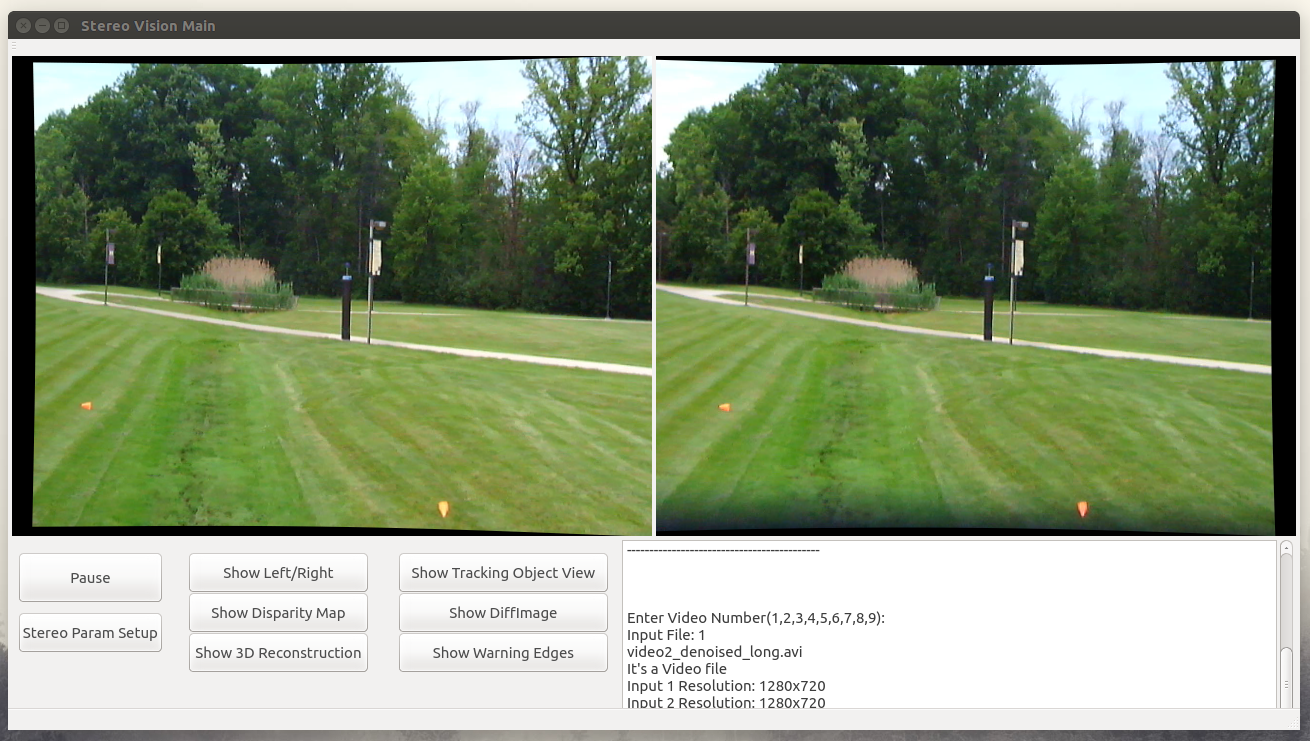
\includegraphics[scale=0.35]{./Resources/gui_showleftright_view.png}
 	\caption{Captura da Tela da Interface Gráfica - Visualização simultânea dos quadros das câmeras esquerda e direita}
 	\label{gui_showleftright_view}
\end{figure}


\begin{figure}[H]
 	\centering
 	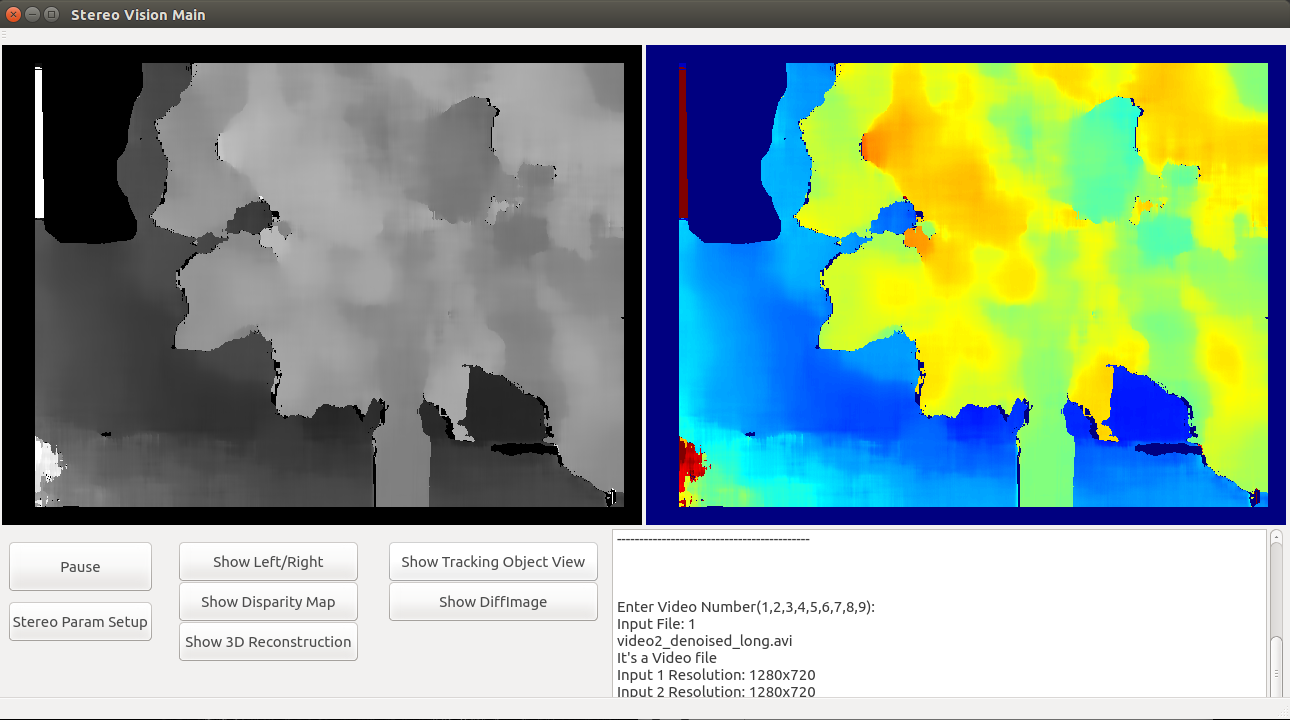
\includegraphics[scale=0.35]{./Resources/gui_showdisparitymap_view.png}
 	\caption{Captura da Tela da Interface Gráfica - Visualização dos Mapa de disparidades em Escala de Cinza e RGB}
 	\label{gui_showdisparitymap_view}
\end{figure}


\begin{figure}[H]
 	\centering
 	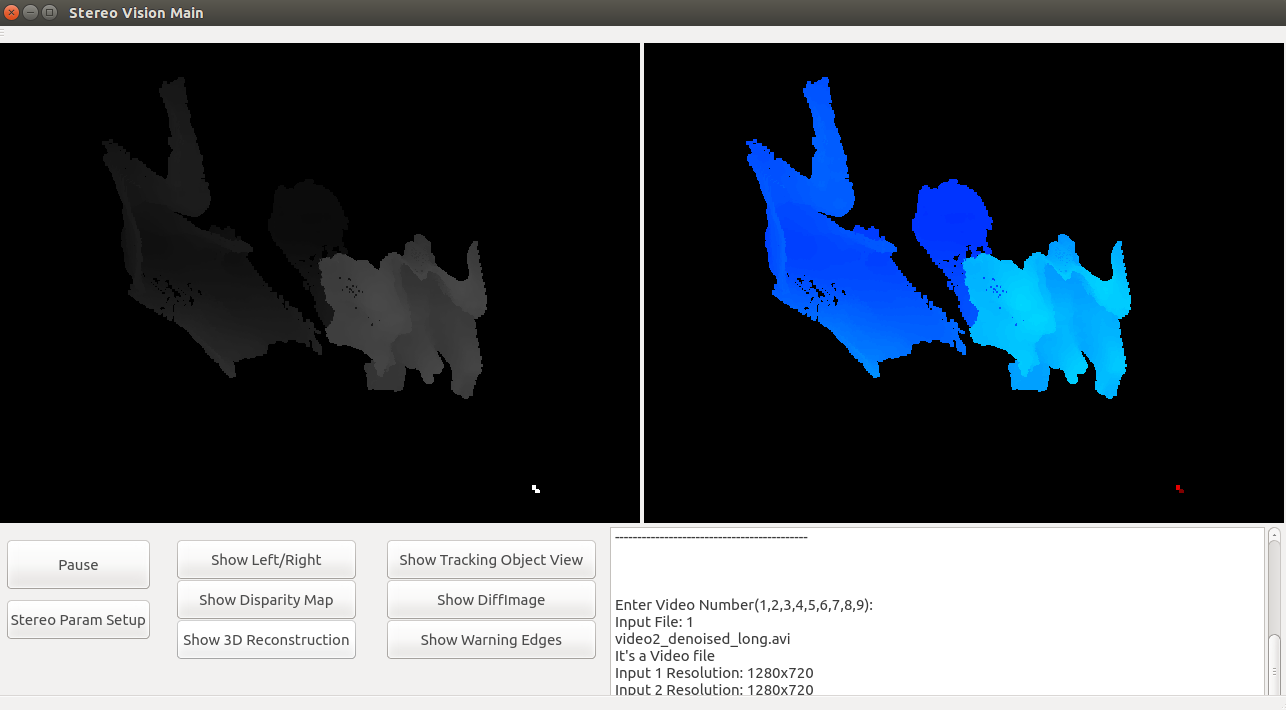
\includegraphics[scale=0.35]{./Resources/gui_show3dreconstruction_view.png}
 	\caption{Captura da Tela da Interface Gráfica - Visualização dos Mapa de disparidades em Escala de Cinza e RGB}
 	\label{gui_show3dreconstruction_view}
\end{figure}


\begin{figure}[H]
 	\centering
 	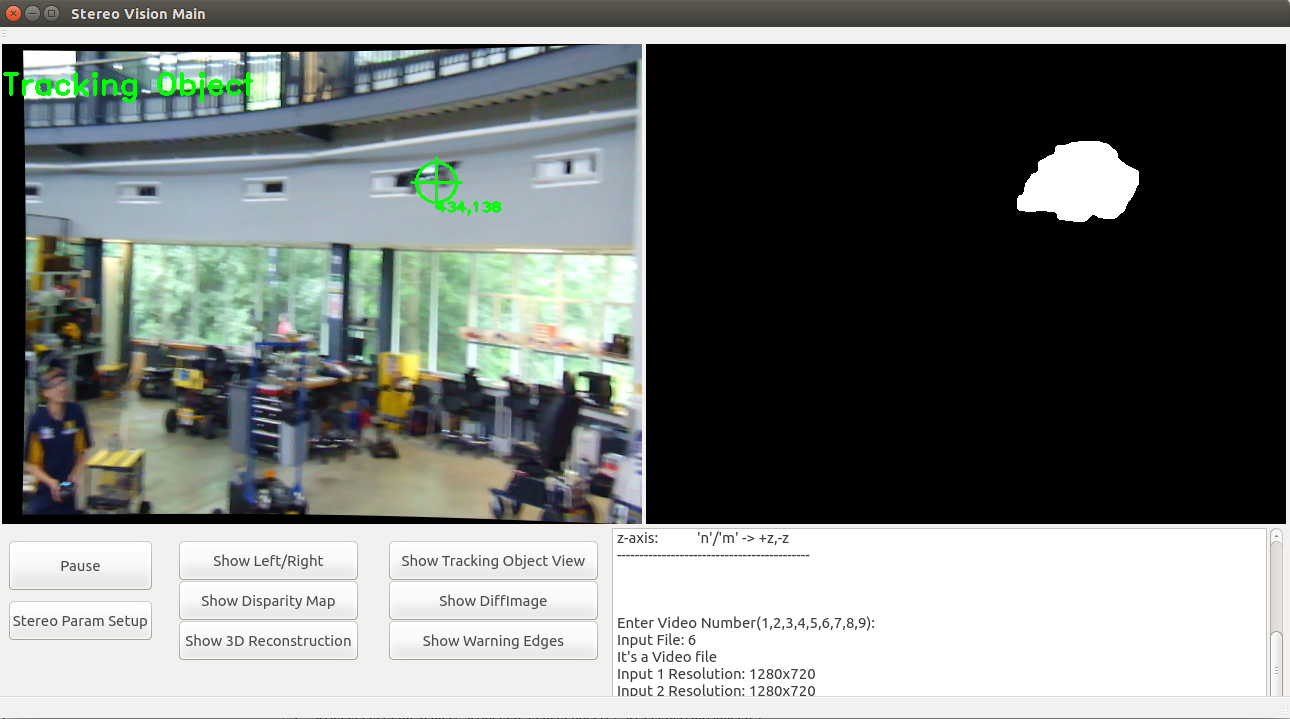
\includegraphics[scale=0.35]{./Resources/gui_show_tracking_object_view.png}
 	\caption{Captura da Tela da Interface Gráfica - Visualização da Imagem da Câmera Esquerda com o indicador de objeto rastreado e da Imagem binária resultante da limiarização por distância}
 	\label{gui_show_tracking_object_view}
\end{figure}


\begin{figure}[H]
 	\centering
 	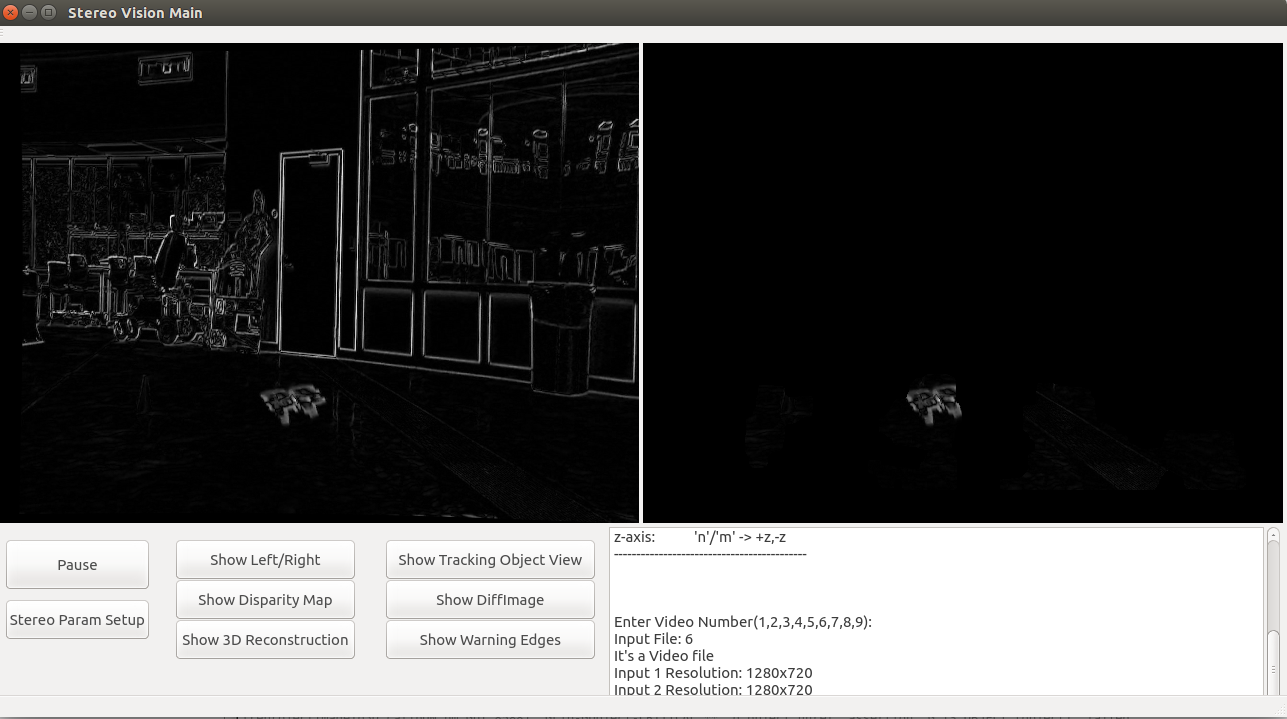
\includegraphics[scale=0.35]{./Resources/gui_showdiffimage_view.png}
 	\caption{Captura da Tela da Interface Gráfica - Visualização da imagem resultante do processo de detecção de movimentos e imagem resultante do processo de detecção de movimentos limiarizada por distância}
 	\label{gui_showdiffimage_view}
\end{figure}


\begin{figure}[H]
 	\centering
 	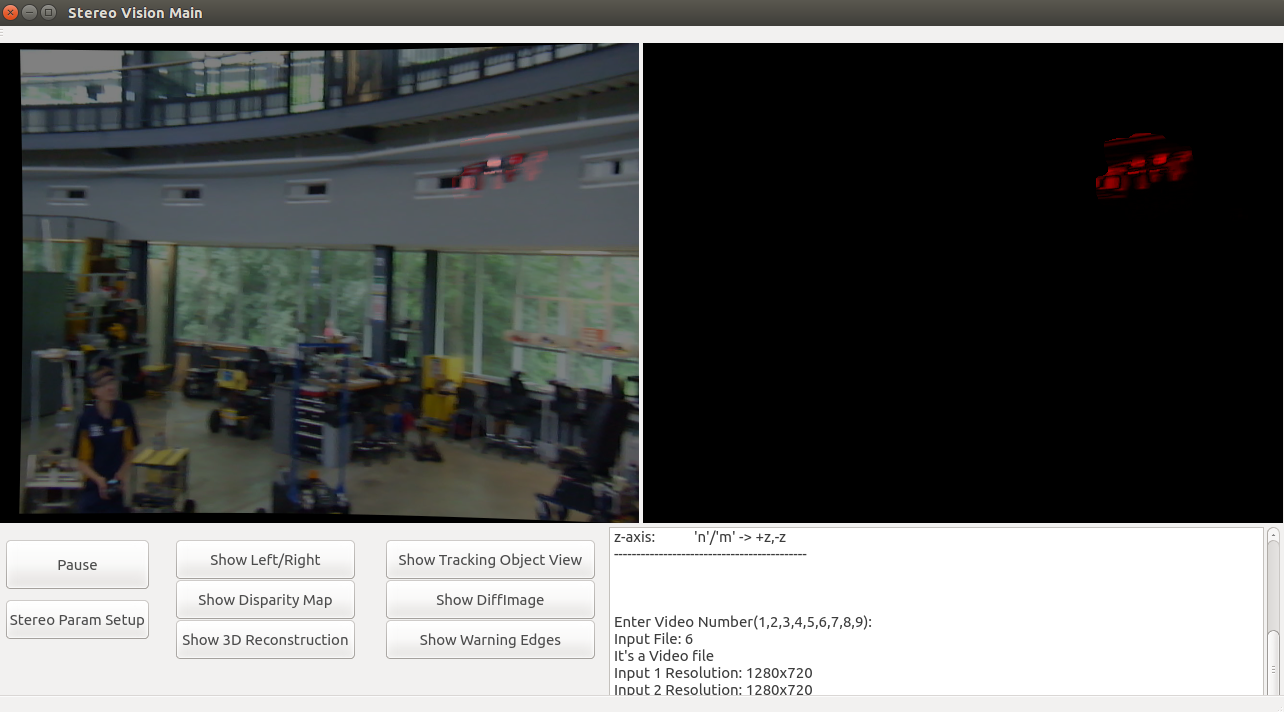
\includegraphics[scale=0.35]{./Resources/gui_showwarningedges_view.png}
 	\caption{Captura da Tela da Interface Gráfica - Visualização da Imagem resultante da adição da imagem à direita com a Imagem da Câmera Esquerda e Imagem resultante do processo de realce das bordas dos 
 	objetos em movimento próximos ao veículo}
 	\label{gui_showwarningedges_view}
\end{figure}


%-----------------------------------------------------------------------------------------------------------------------------------------------------------------------------------------------
\section{Cenários - Resultados Visuais}
\label{resultsScenes}

Nesta seção, estão apresentados os resultados obtidos de cada método estéreo para os cenários propostos na seção \ref{scenes}. Para facilitar a comparação dos mapas de disparidades foi apresentado uma colagem para cada cenário, contendo o par de imagens capturadas da cena, o mapa de disparidade em nível de cinza e em RGB para os métodos BM, SGBM e BMGPU, respectivamente. As regiões que não contêm informações (regiões com grandes porções de cor escura, no caso da imagem RGB, de cor azul-marinho) estão muito próximas às câmeras ou áreas com superfícies refletivas. Nestas superfícies, os métodos estéreo apresentam baixa relação de unicidade, isto é, a cada iteração, mesmo em uma cena parada, o método apresenta dificuldade para definir os corretos valores de correspondências. Deste modo, é preferível identificá-las e desconsiderá-las do mapa de disparidades.

Como apresentado pela figura \ref{scene1_montage}, a árvore é tida como principal obstáculo nesta cena e todos os métodos conseguiram identificá-la e realçá-la corretamente. O método SGBM apresenta cores mais frias, pois a configuração que permitia a correta segmentação do objeto apresenta um maior número de níveis de cinza para o mapa de disparidades. No caso do Método BMGPU, temos uma elevada porcentagem de região desconhecida, porém este consegue identificar essas regiões ao passo que o veículo se aproxima dessas regiões. 

Na figura \ref{scene2_montage}, é possível observar que o Método SGBM, diferentemente dos métodos BM e BMGPU, conseguiu identificar as bancadas, as regiões muito próximas ao quadricóptero e o cone de segurança, e não apenas as bancadas como ocorreu nos outros métodos. Entretanto, vale lembrar que este método é pesado computacionalmente e a performance do sistema também deve ser tomado em conta, não somente a qualidade do mapa gerado. 

Os resultados obtidos para o terceiro cenário proposto está ilustrado pela figura \ref{scene3_montage}. Nela foi possível, observar que todos os métodos foram capazes de identificar o piloto e o quadricóptero. Este resultado é bastante importante, visto que se provou que é possível utilizar visão estéreo para a identificação não somente de obstáculos estáticos, como também obstáculos dinâmicos, sendo estes terrestres ou aéreos. O aperfeiçoamento dos equipamentos para detecção de objetos por intermédio de visão estéreo é um dos passos que talvez possibilitem \textit{drones} a utilizar o tráfego aéreo. 

\begin{figure}[H]
 	\centering
 	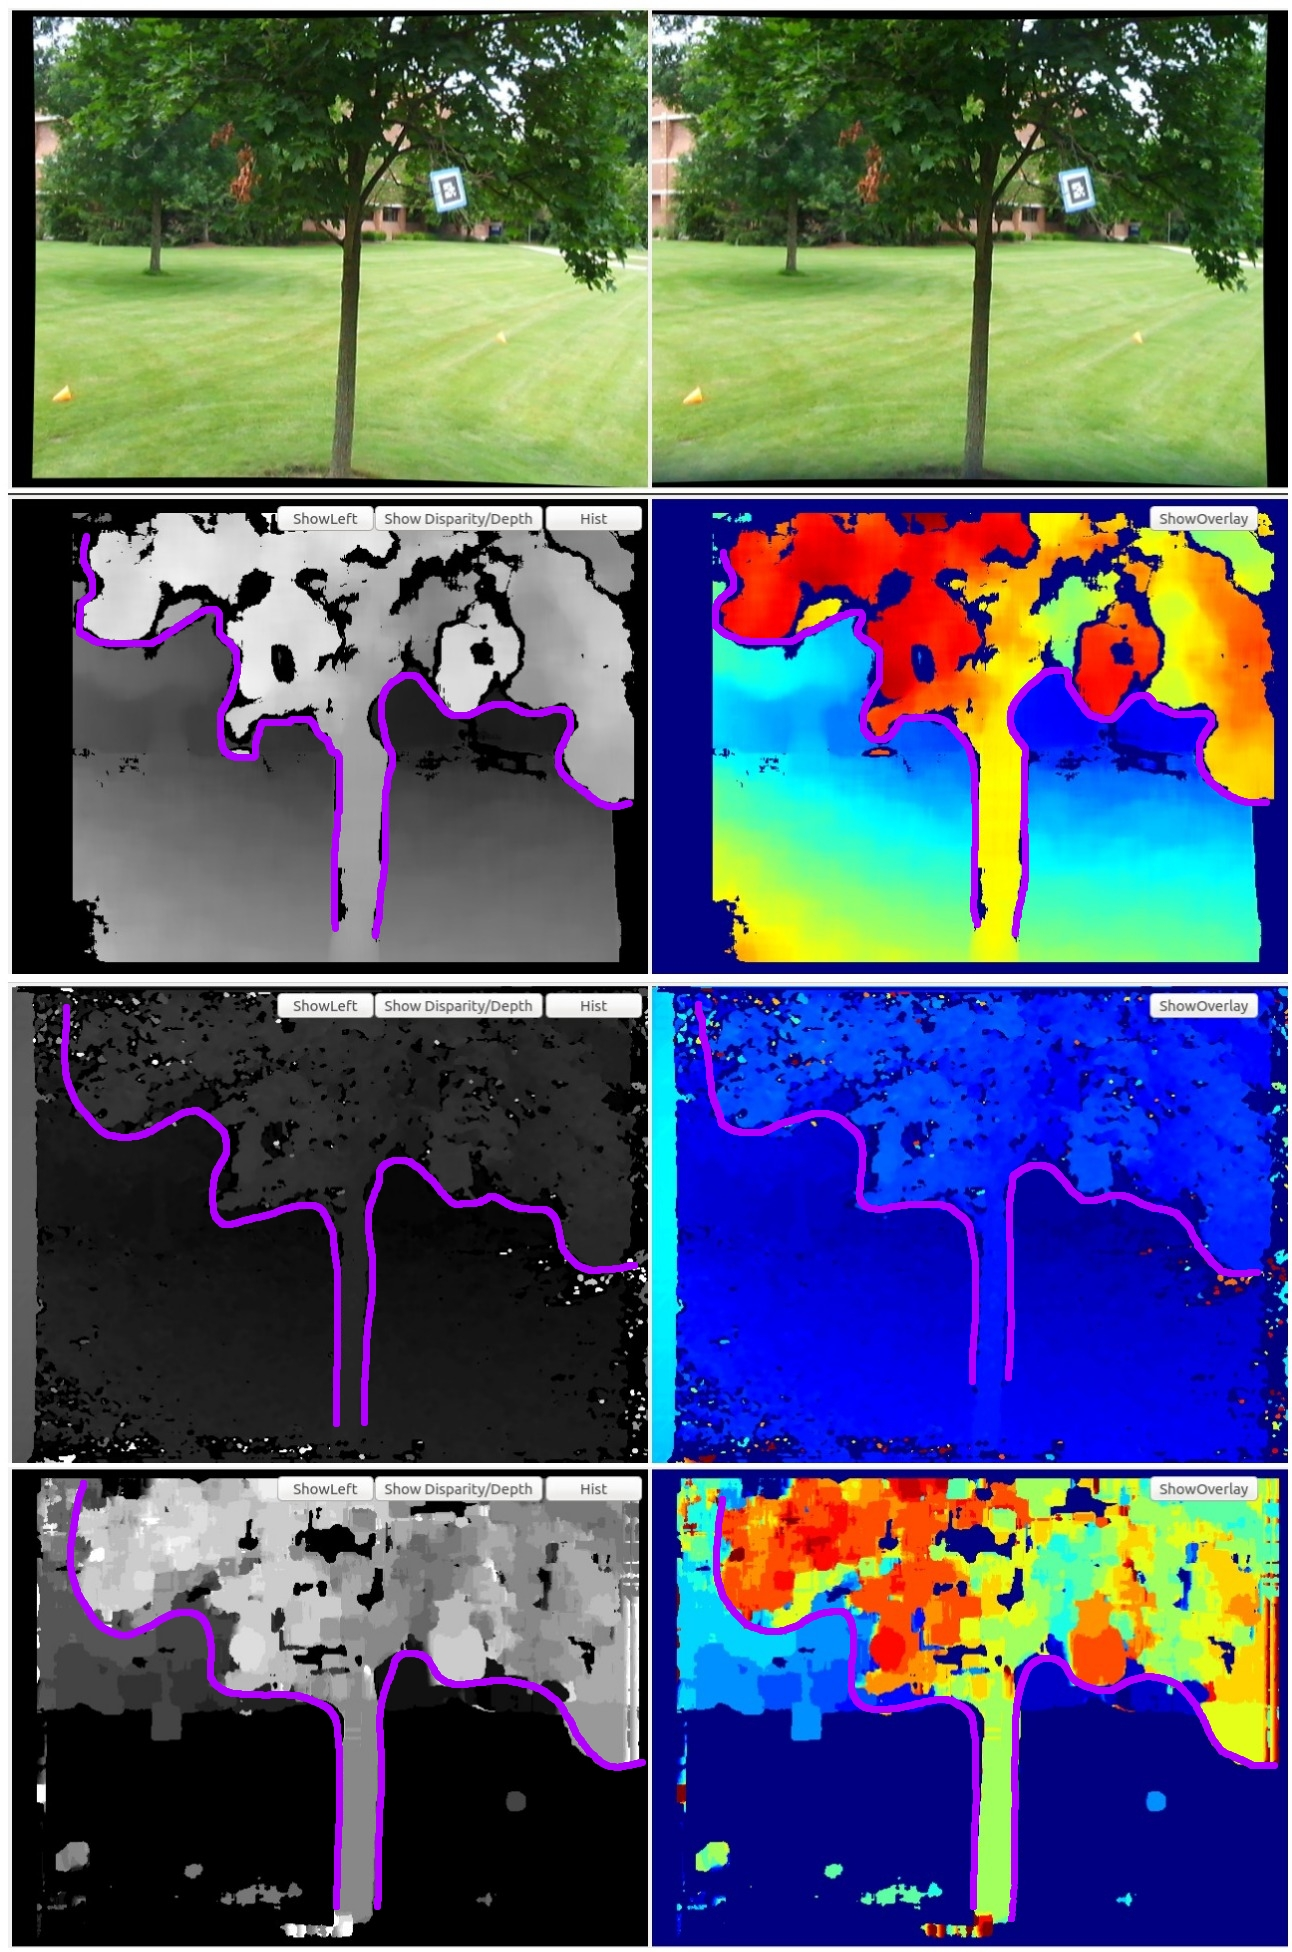
\includegraphics[scale=0.33]{./Resources/results/scene1_montage_highlighted.jpg}
 	\caption{Montagem de capturas de tela refente ao Cenário 1 - Comparativo do Mapa de Disparidades gerado pelos Métodos BM, SGBM e BMGPU, respectivamente. Árvore como principal obstáculo.}
 	\label{scene1_montage}
\end{figure}

\begin{figure}[H]
 	\centering
 	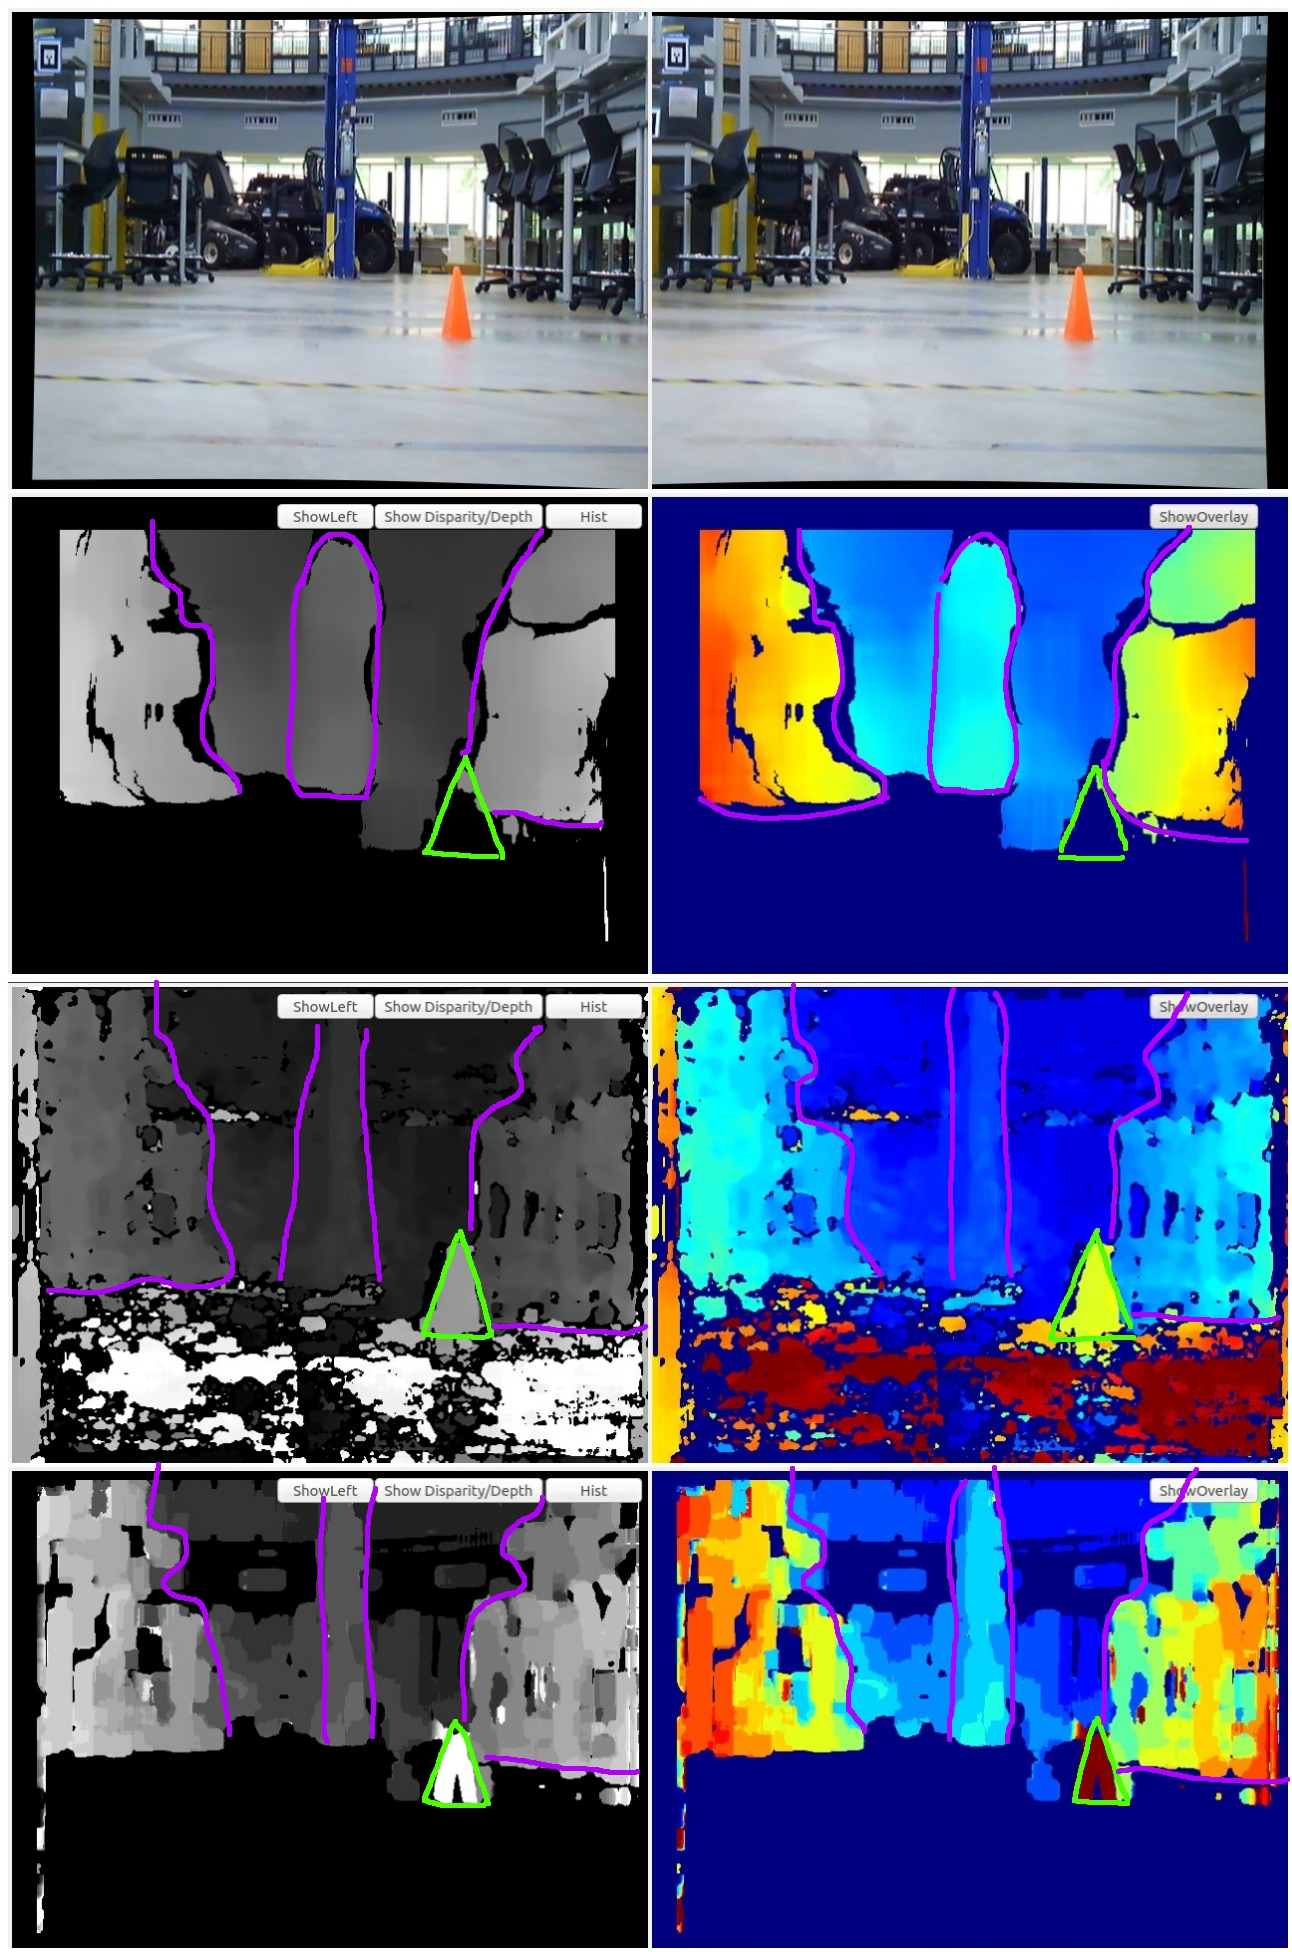
\includegraphics[scale=0.33]{./Resources/results/scene2_montage_highlighted.jpg}
 	\caption{Montagem de capturas de tela refente ao Cenário 2 - Comparativo do Mapa de Disparidades gerados pelos Métodos BM, SGBM e BMGPU, respectivamente. Bancadas, Cone de segurança como principais obstáculos.}
 	\label{scene2_montage}
\end{figure}

\begin{figure}[H]
 	\centering
 	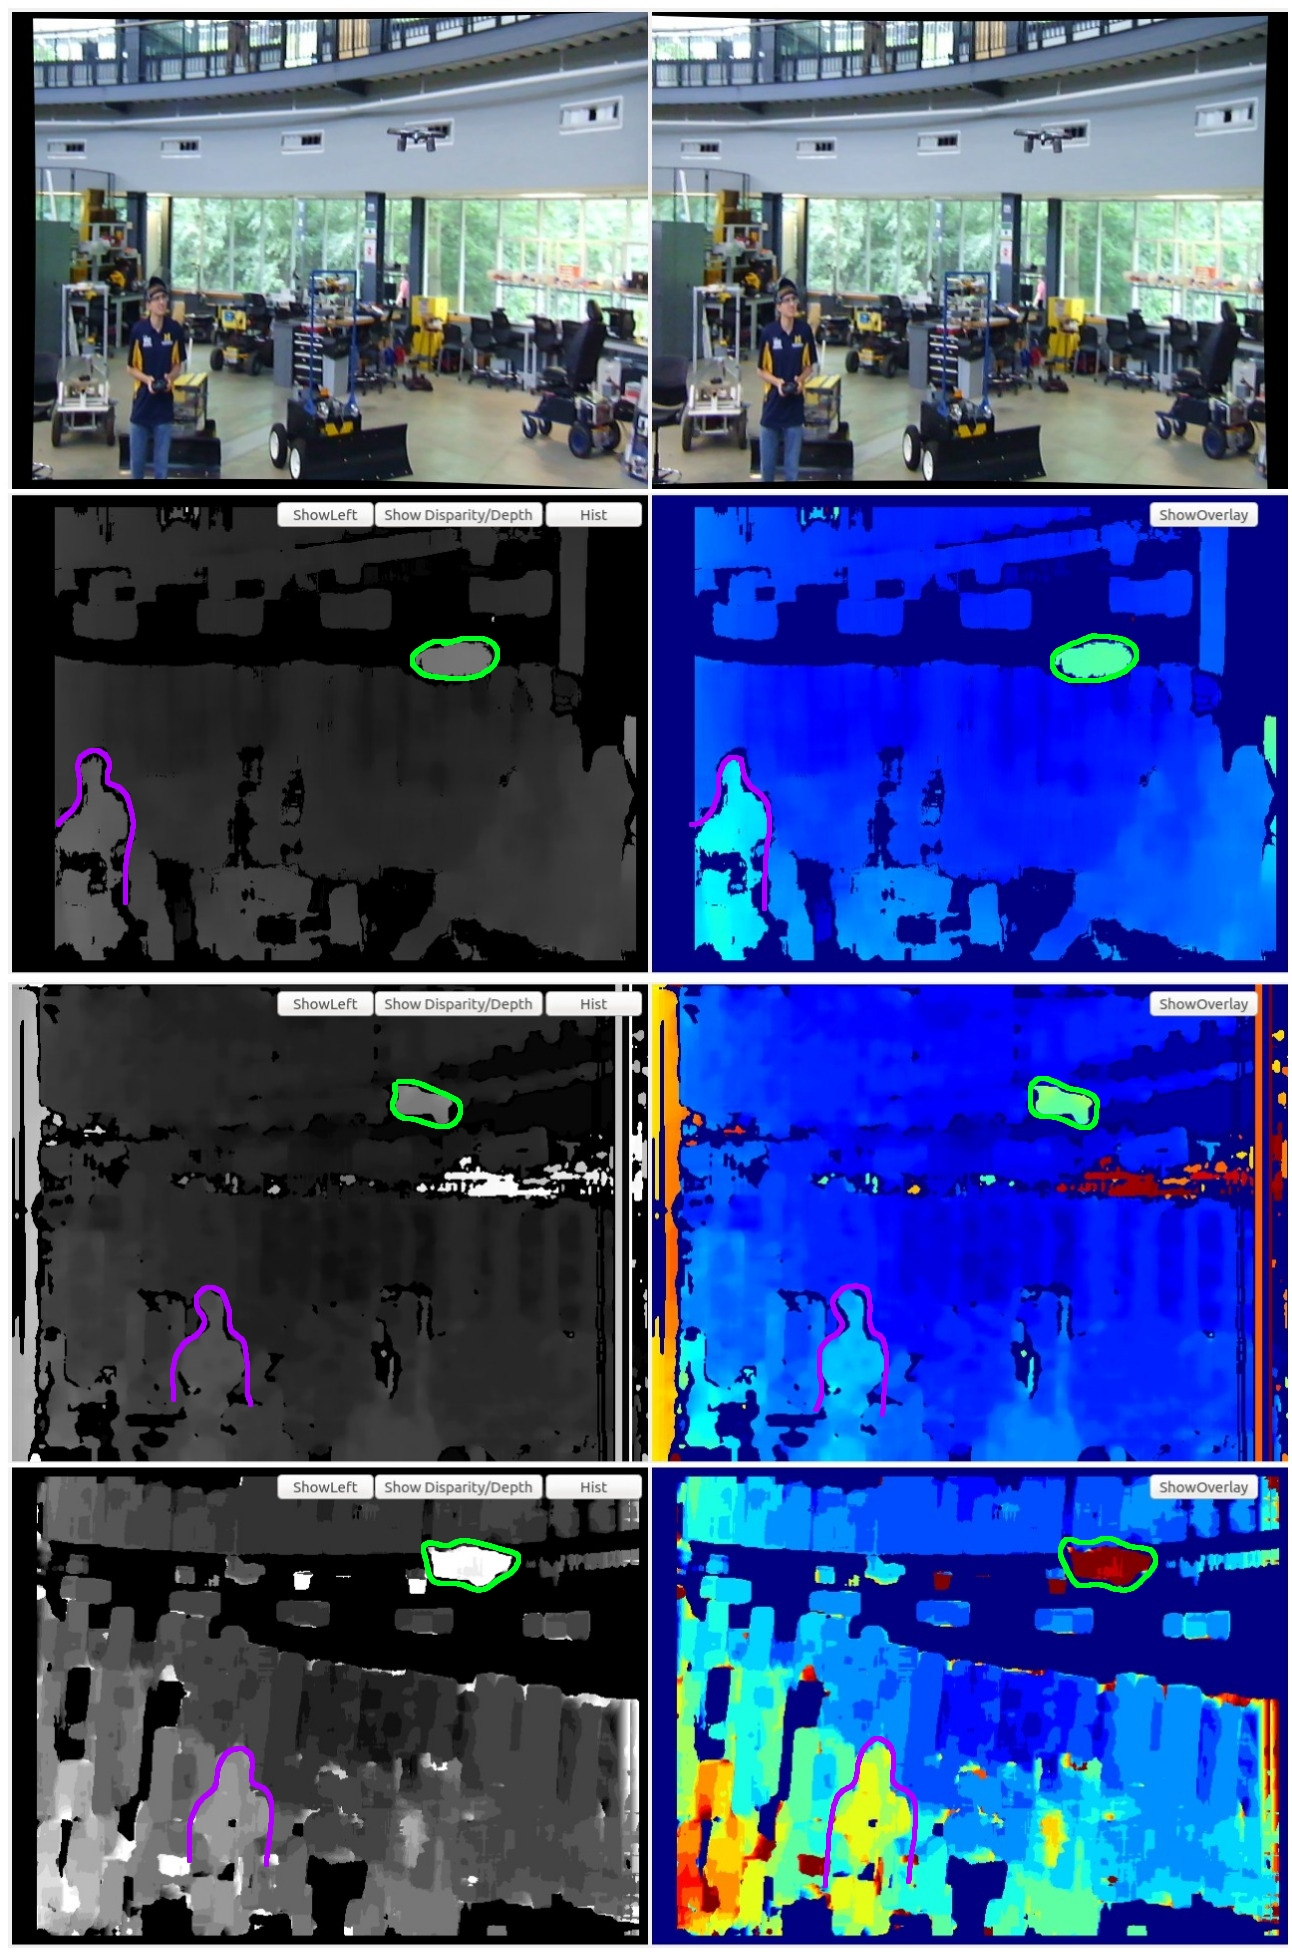
\includegraphics[scale=0.33]{./Resources/results/scene3_montage_highlighted.jpg}
 	\caption{Montagem de Capturas de Tela refente ao Cenário 3 - Comparativo do Mapa de Disparidades gerados pelos Métodos BM, SGBM e BMGPU, respectivamente. Piloto e Veículo aéreo (Quadricóptero) como principais obstáculos.}
 	\label{scene3_montage}
\end{figure}

%-----------------------------------------------------------------------------------------------------------------------------------------------------------------------------------------------
\section{Comparação de Desempenho: Desktop x BBB x Jetson TK1}
\label{resultsComparison}

Nesta seção, estão apresentados os resultados práticos das diferentes implementações dos métodos de visão estéreo nas plataformas abordadas. Os Métodos utilizados foram BM, SGBM e BMGPU para a comparação das plataformas. O método BMGPU mostrou-se o de melhor performance, visto que é o que requisita menor processamento dentre os outros métodos mais conhecidos (SGBM, BP, CSBP, AD Census, ...) além de ser acelerado em hardware. 

Com relação à configuração utilizada para a realização dos testes, utilizou-se uma resolução de 640x480, um tamanho médio da janela usada para combinar blocos de pixels (\textit{SADWindowSize}) de 15 e um tamanho da gama de disparidades (\textit{NumberOfDisparities}) igual à 16, como pode ser observado na tabela \ref{teste_values}. O parâmetro \textit{SADWindowSize} pode assumir valores ímpares dentro do intervalo [5,255] e o parâmetro \textit{NumberOfDisparities} só de assumir valores múltiplos de 16 no intervalo [16,256]. O critério de escolha desses valores foi dado pelo balanço entre performance e qualidade do mapa de disparidades gerado, isto é, um mapa que fosse confiável e permitisse as corretas correspondências do mapa de disparidades. Os parâmetros \textit{preFilterSize}, \textit{preFilterCap}, \textit{minDisparity}, \textit{textureThreshold}, \textit{uniquelessRatio}, \textit{speckleWindowSize}, \textit{speckleRange} e \textit{disp12MaxDiff} também configuram os métodos estéreo, porém não impactam no desempenho do método como os parâmetros anteriores. A tabela \ref{resultsCPUGPU} abaixo, apresenta o resultado de desempenhos obtidos nas plataformas, apresentando comparativamente seu desempenho quando o processado utilizando CPU ou GPU/NEON (Caso da BBB).

\begin{table}[h]
\centering
\caption{Configuração utilizada para Avaliação de Performance}
\label{teste_values}
\begin{tabular}{|c|c|}
\hline
                    & Configuração \\ \hline
Resolução           & 640x480      \\ \hline
SADWindowSize       & 15           \\ \hline
NumberOfDisparities & 16           \\ \hline
\end{tabular}
\end{table}

\begin{table}[h]
\centering
\caption{Desempenho atingido por cada plataforma dos Métodos Utilizados}
\label{resultsCPUGPU}
\begin{tabular}{|c|c|c|c|}
\hline
Quadros por Segundo (FPS)       & BM & SGBM & BM\_GPU  \\ \hline
Desktop   & 28 & 12   & 30       \\ \hline
BBB       & 1  & -    & -        \\ \hline
Jetson TK1 & 6  & 2    & 7$\sim$8 \\ \hline
\end{tabular}
\end{table}

O gráfico da figura \ref{grafico_desempenho} apresenta o comparativo entre o desempenho de cada plataforma para os métodos estéreo BM, SGBM e BMGPU. O resultado da BBB para o método BM é muito inferior aos resultados obtidos nas demais plataformas. O teste para o método SGBM foi abortado, visto que naturalmente este método é um algoritmo mais complexo que o BM. Decorrente a isso, espera-se que sua performance seja inferior à um FPS. Segundo o manual da BBB, o processador ARM Cortex A8 apresenta suporte ao NEON™, o qual é um acelerador de ponto flutuante que utiliza instruções SIMD (\textit{Single instruction, Multiple Data}) para a aceleração de algoritmos de multimídia e processamento de sinais \cite{ARMNEON}. Os testes dos métodos estéreo na BBB utilizando essa tecnologia também não foram executados, pois sua implementação tomaria um tempo considerável e provavelmente não apresentaria um resultado expressivo. 

\begin{figure}[H]
 	\centering
 	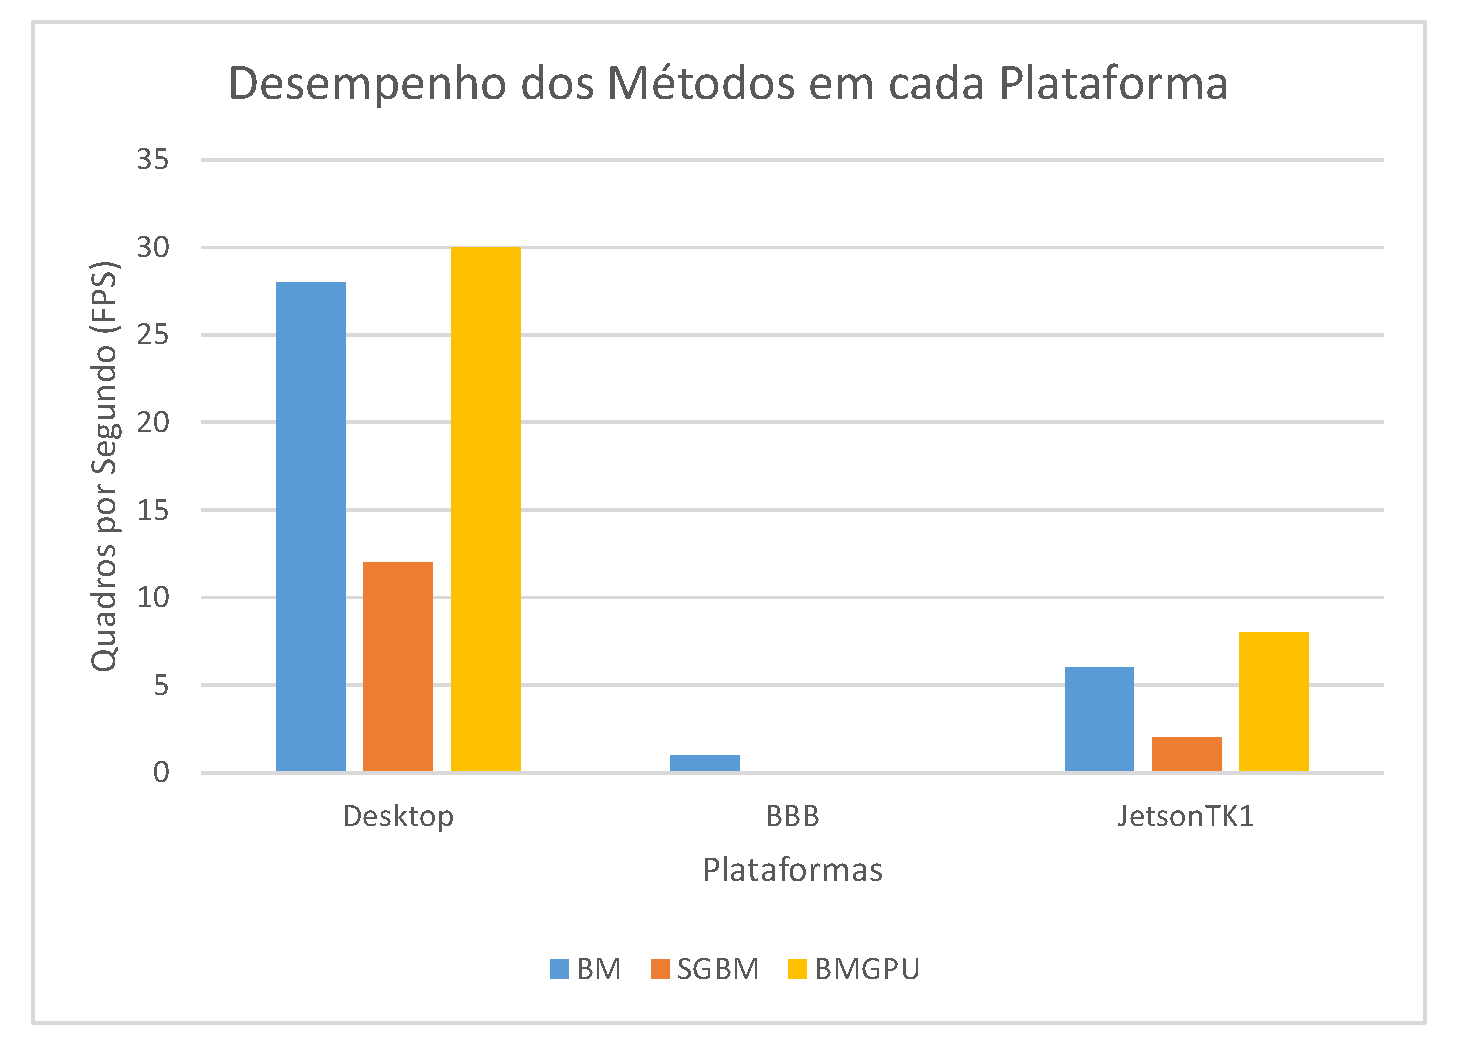
\includegraphics[scale=0.5]{./Resources/grafico_desempenho.pdf}
 	\caption{Gráfico - Comparação de Desempenho dos Métodos Estéreo para cada plataforma.}
 	\label{grafico_desempenho}
\end{figure}

Este trabalho não tem como escopo realizar a avaliação dos resultados apresentados acima com relação ao atendimento dos requisitos da aplicação. O trabalho realiza a busca pelas limitações dos sistemas para a execução dos métodos estéreo. No que diz respeito às condições do teste, em nenhuma das plataformas realizou-se a prioritização dos processos no sistema. Vale realçar que nenhuma distribuição do tipo RTOS (Sistema Operacional em Tempo Real) foi utilizada.

%-----------------------------------------------------------------------------------------------------------------------------------------------------------------------------------------------
\subsection{Desktop}
\subsubsection{CPU}

Primeiramente, as rotinas para execução em CPU foram implementadas no \textit{Desktop} e só então foram adaptadas para as plataformas embarcadas. Os valores de desempenho obtidos foram usados como referência para a comparação com os resultados acelerados por GPU e com as plataformas embarcadas. Como esperado, o SGBM mostrou-se mais lento que o BM, isso deve-se ao fato do algoritmo ser mais complexo por conta da análise global realizada (Mais detalhes em \ref{stereo_methods}). 

\subsubsection{GPU}

Como previsto, o desempenho do método BM acelerado em GPU é superior ao executado em CPU. O ganho em desempenho é pequeno, isto deve-se ao fato do tempo necessário para transferir as imagens entre a memória utilizada pela CPU e a memória da GPU é comparativamente grande ao ganho de processamento pela execução em GPU. Consequentemente, este resultado motivou a implementação do mesmo na plataforma \textit{Jetson TK1}, visto que sua implementação é bastante similar a em Desktop por conta de possuírem a mesma arquitetura de GPU (Kepler).  


%-----------------------------------------------------------------------------------------------------------------------------------------------------------------------------------------------
\subsection{BeagleBone Black (BBB)}
\subsubsection{CPU}

O resultado obtido para o método BM desmotivou qualquer outra implementação nesta plataforma. Dificilmente, algum outro recurso de aceleração apresentaria um resultado que realizasse o processamento de imagens necessários com resposta em tempo real. 

\subsubsection{NEON}
Como já fora dito, o resultado obtido pela performance em CPU, desestimulou o estudo e implementação desta tecnologia.


%-----------------------------------------------------------------------------------------------------------------------------------------------------------------------------------------------
\subsection{Jetson TK1}
\subsubsection{CPU}
A implementação em CPU nesta plataforma foi realizada para efeito de comparação entre o desempenho obtido em CPU e com a implementação utilizando CUDA. Como esperado, o método SGBM também se mostrou mais lento que o BM, apresentando uma taxa de processamento relativamente baixa, aproximadamente dois FPS. Com relação ao BM, a taxa atingida foi de aproximadamente seis quadros por segundo. Avaliando o resultado para aplicação em veículos autônomos, essa taxa ainda dificulta aplicações em tempo real, visto que a plataforma simultaneamente estaria executando algoritmos de mapeamento e navegação.

\subsubsection{GPU}
Como esperado, a implementação da tecnologia CUDA na \textit{Jetson TK1} acelerou a execução do método BM em aproximadamente 30\%. Todavia, o ganho obtido representa uma melhora de apenas um ou dois FPS e, assim como dito acima, aplicações que garantam resposta em tempo real necessitam apresentar taxas de processamento muito superiores à essa. Idealmente, espera-se que a taxa de processamento seja pelo menos igual à taxa de captura da câmera.

%-----------------------------------------------------------------------------------------------------------------------------------------------------------------------------------------------
% Conclusões: "fecha" com os objetivos? (respondem aos objetivos?) - aqui é que "se vende o peixe" - elas é que valorizam (ou não) o trabalho realizado.
% Normalmente é uma parte do trabalho "um pouco desprezada", pois o autor já está "cansado....". Mas é aqui que realmente se mede se o trabalho tem ou não valor.
% Contém o item Trabalhos futuros, que é uma orientação sobre as possibilidades de continuação do desenvolvimento do trabalho.
\chapter{Conclusão e Trabalhos Futuros}
\label{Conclusao}

\section{Conclusão}
O trabalho cumpriu todos os objetivos apresentados na seção \ref{objetivos}. 

No que diz respeito à visão estéreo, foram realizados o estudo e a aplicação das técnicas de visão computacional para o problema proposto, mais precisamente estudou-se os processos de calibração, retificação, filtragem e os métodos estéreo para a obtenção de um mapa de disparidades denso. 

No que concerne o monitoramento de um veículo autônomo, foi desenvolvida uma plataforma de apoio que facilita o processo de calibração dos métodos estéreo para as plataformas embarcadas, visto que são destinadas a uma aplicação que não necessita de interface gráfica. Além disso, ela possibilita o monitoramento via estação-base, caso deseja-se que o processamento das imagens não seja realizado \textit{on-board}. Os métodos foram implementados e testados em cenários capturados pela câmera fixada no quadricóptero. Entretanto, a extensão desse trabalho não se resume a veículos aéreos, as plataformas utilizadas podem muito bem serem empregadas em veículos terrestres e até mesmo em veículos aquáticos, evidentemente com a devida vedação dos equipamentos. Outro importante objetivo foi a comparação de desempenho dos métodos nas plataformas disponíveis, BBB e Jetson TK1. No caso da BBB, mesmo a rotina desenvolvida mostrando-se totalmente funcional, isto é, os algoritmos conseguem detectar e segmentar relativamente bem os obstáculos dos cenários propostos, ocorreu que a taxa de processamento tornou-se uma preocupação. O desempenho foi extremamente baixo, aproximadamente um quadro por segundo, o que claramente inviabiliza sua utilização em uma aplicação real. A alteração de plataforma mostrava-se ser uma solução para o aumento da taxa de atualização, visto que a Jetson TK1 é uma plataforma mais recente e mais poderosa. O desempenho desenvolvido pela Jetson TK1 foi de aproximadamente seis FPS (Método BM), performance ainda baixa para um sistema que deve apresentar resposta em tempo real (O critério de avaliação tomado foi de pelo menos 10 FPS).

Diante deste impasse, duas providências foram cruciais para a continuidade do trabalho. A primeira foi a otimização das rotinas utilizadas, sendo essa uma tentativa para a melhora do desempenho geral dos métodos. A segunda foi a execução de uma ampla revisão bibliográfica, incluindo principalmente trabalhos que apresentassem comparativos de desempenho entre plataformas e que tivessem realizados algum tipo de aceleração por \textit{hardware}, sejam eles envolvendo paralelização de processos, implementação em FPGA ou utilizando a plataforma de computação paralela CUDA. Ao fim, a última alternativa foi tomada visto que a plataforma Jetson TK1 apresenta suporte a tecnologia CUDA.

Com relação à utilização de uma plataforma embarcada em quadricóptero, a plataforma Jetson TK1 juntamente com o método BMGPU foi a melhor alternativa para a implementação em um sistema real, mesmo apresentando uma taxa de performance reduzida, foi a melhor solução existente durante o período de desenvolvimento do trabalho. Vale ressaltar que as rotinas implementadas utilizaram os métodos estéreo presentes no OpenCV, isto é, não se desenvolveu rotinas em programação CUDA, diretivas para a manipulação de dados em GPU. Deste modo, existe a expectativa de que essas bibliotecas sejam otimizadas em novas versões do OpenCV ou que a NVIDIA atualize a versão do CUDA \textit{Toolkit}, reduzindo assim o tempo de execução.

Quanto à qualidade do mapa de disparidades, a câmera utilizada, FinePix 3D W3, mesmo sendo uma câmera comercial que não necessariamente precisa se preocupar com o perfeito alinhamento do \textit{Stereo Rig} e qualidade das lentes apresentou resultados satisfatórios, isto é, mapas com as corretas correspondências dos pontos homôlogos e com baixa porcentagem de região de desconhecido. Com o devido processo de calibração foi capaz de capturar os vídeos utilizados para o desenvolvimento desse trabalho, além de cumprir todos os requisitos do projeto (Leve, \textit{Baseline} rígida, Taxa de quadros elevada).

Em suma, o projeto atendeu seus principais objetivos e proporcionou o estudo de diferentes conceitos essencialmente relacionados com visão computacional, sistemas embarcados e aceleração em GPU. Com relação aos mapas de disparidades gerados pelos métodos estéreo, os resultados obtidos, tanto em CPU quanto em GPU, são idênticos, porém ainda se apresentam problemas referentes à performance do sistema. Por hora, eles podem ser resolvidos com a substituição dos equipamentos por melhores câmeras ou plataformas embarcadas mais poderosas. Ao fim do trabalho, os algoritmos desenvolvidos podem ser totalmente adaptados para a sua incorporação a sistemas robóticos mais conhecidos como \textit{Player/Stage} \cite{Gerkey2010}, \textit{Gazebo} \cite{Gazebo}, \textit{ROS} \cite{ROS}, dentre outros. Esse tipo de integração pode ser realizada modificando-se a plataforma desenvolvida para que esta publique corretamente as imagens nos tópicos do ROS, por exemplo. Os resultados obtidos permitiram que uma nova fase de pesquisa se iniciasse e também possibilitasse o estudo de novos conceitos como SLAM, algoritmos para desvio de obstáculos, planejamento de rotas.

\section{Trabalhos Futuros}

Como apresentado acima, concluiu-se que o trabalho desenvolvido apresentou bons resultados em diversos aspectos, porém esses resultados podem ser melhorados pela simples troca ou atualização das câmeras e plataformas utilizadas. Além disso, ao fim do desenvolvimento do projeto, indagou-se quais modificações deveriam ser realizadas para a real implementação do sistema autônomo. Consequentemente, a maior parte das sugestões de atividades futuras descritas nessa seção estão diretamente relacionadas com as possíveis melhorias e implementação de novos conceitos.

No que se refere à atualização de plataformas, a NVIDIA lançou recentemente uma nova plataforma - Jetson TX1 que apresenta um aumento expressivo de núcleos CUDA, aproximadamente 30\% em relação à versão anterior \cite{JetsonTX1}. A implementação do trabalho desenvolvido nesta nova plataforma é bastante válida e interessante, visto que existe a possibilidade da melhora na performance do sistema. Além disso, o estudo de novas alternativas de aceleração em \textit{hardware} também é válido. Uma delas é a utilização de FPGAs, as quais são dispositivos que possibilitam o desenvolvimento de arquiteturas totalmente especializadas e também podem ser dedicadas a esse tipo de aplicação, como visto em \cite{Barry2015}. Outra alternativa ainda mais recente, seria a utilização da tecnologia presente nos processadores gráficos Mali™ da ARM \textregistered. Eles também permitem a aceleração em GPU, com um elevado grau de especialização, por meio da utilização de programação paralela OpenCL \cite{StereoARM}. Ambas arquiteturas apoiam-se na utilização de \textit{pipelines}, as quais proporcionam que mais de um processo sejam executados comitantemente, o que reduz drasticamente o tempo para a execução de cada quadro. Embora a Jetson TK1 suporte à tecnologia CUDA, ela ainda é uma plataforma de desenvolvimento e de propósito geral, por conta disso, acredita-se que o desempenho das alternativas apresentadas sejam melhores.

No que diz respeito à atualização das câmeras, existem atualmente no mercado algumas câmeras que também cumprem todos os requisitos do projeto e poderia muito bem serem incorporadas. As câmeras estéro mais indicadas para esse tipo de aplicação são a \textit{Bumblebee\textregistered2} da \textit{Point Grey Research} \cite{bumblebee2}, \textit{ZED™} da \textit{StereoLabs} \cite{StereoLabsZED} e as câmeras \textit{DUO 3D™} da \textit{Code Laboratories} \cite{CodeLaboratoriesDUO}. Cada qual possui sua especialidade: Alta taxa de quadros, Alta Resolução, Tamanho Pequeno, respectivamente. Atualmente, a StereoLab e a NVIDIA têm colaborado para o desenvolvimento de sistemas que utilizem a câmera ZED™ e as plataformas da família Jetson, o que realmente incentiva a comunidade de desenvolvedores optarem por essa solução \cite{NVIDIAStereoLabsPartenership}. Isso é um indicativo que o caminho para o desenvolvimento de plataformas embarcadas utilizando visão estéreo será mediante à combinação de equipamentos dessas empresas.



%------------------------------------- Adição das Bibliografias -------------------------------------	
\bibliographystyle{unsrt} 			% Define o estilo da bibliografia
% \bibliographystyle{ieeetr} 			% Define o estilo da bibliografia
\bibliography{./Content/References} 		% Faz referência ao arquivo ref.bib

%------------------------------------- Configurações de Anexos --------------------------------------
\newcommand{\annexname}{Anexo}
\makeatletter
\newcommand\annex{\par
  \setcounter{chapter}{0}
  \setcounter{section}{0}
  \gdef\@chapapp{\annexname}
  \gdef\thechapter{\@Roman\c@chapter}}
\makeatother

\newenvironment{poliabstract}[1]
  {\renewcommand{\abstractname}{#1}\begin{abstract}}
  {\end{abstract}}

%------------------------------------- Adição dos Anexos -------------------------------------------- 	
%\begin{appendices}
\appendix
%------------------------------------- Apêndice 1 ---------------------------------------------------
\chapter{Apêndice 1}
\label{Apendice1}
% Dica:
% APÊNDICE -- Documento ou texto elaborado pelo autor
% ANEXO	   -- Documento ou texto não elaborado pelo autor

Todos os trechos de código desenvolvidos e os arquivos de calibração utilizados para a estação-base da interface gráfica e para as outras plataformas podem ser encontradas nos seguintes repositórios:

\begin{itemize}
 \item Desktop: \url{https://github.com/nicolasrosa/StereoVision}
 \item BBB: \url{https://github.com/nicolasrosa/StereoVisionBBB}
 \item Jetson TK1: \url{https://github.com/nicolasrosa/StereoVisionJetsonTK1}
\end{itemize}
%\end{appendices}

\annex
%------------------------------------- Anexo 1 ------------------------------------------------------
\chapter{Anexo 1}
\label{Anexo1}

Os seguintes trechos de código foram incorporados ao projeto da interface gráfica para a estação-base. Duas funcionalidades foram adicionadas ao código. A primeira funcionalidade corresponde a parte de reconstrução tridimensional e renderização da nuvem de pontos \cite{UEDA2011}. A segunda funcionalidade corresponde a parte de rastreamento do objeto desenvolvida por Kyle Hounslow \cite{Hounslow2013}. 

\medskip
\lstset {language=C++}
\textbf{3DReconstruction.h}
\begin{lstlisting}[basicstyle=\tiny]
#ifndef RECONSTRUCTION_3D_H
#define RECONSTRUCTION_3D_H

/* Libraries */
#include "opencv2/opencv.hpp"

using namespace cv;
using namespace std;

/* 3D Reconstruction Classes */
template <class T>
static void projectImagefromXYZ_(Mat& image, Mat& destimage, Mat& disp, 
				 Mat& destdisp, Mat& xyz, Mat& R, Mat& t, 
				 Mat& K, Mat& dist, Mat& mask, bool isSub);

template <class T>
static void fillOcclusionInv_(Mat& src, T invalidvalue);

template <class T>
static void fillOcclusion_(Mat& src, T invalidvalue);

// 3D Reconstruction
class Reconstruction3D{
public:
    Reconstruction3D(); //Constructor
    void setViewPoint(double x,double y,double z);
    void setLookAtPoint(double x,double y,double z);
    void PointCloudInit(double baseline,bool isSub);

    /* 3D Reconstruction Functions */
    void eular2rot(double yaw,double pitch, double roll,Mat& dest);
    void lookat(Point3d from, Point3d to, Mat& destR);
    void projectImagefromXYZ(Mat &image, Mat &destimage, Mat &disp, 
			     Mat &destdisp, Mat &xyz, Mat &R, Mat &t,
			     Mat &K, Mat &dist, bool isSub);
    void fillOcclusion(Mat& src, int invalidvalue, bool isInv);


    Mat disp3Dviewer;
    Mat disp3D;
    Mat disp3D_8U;
    Mat disp3D_BGR;

    Point3d viewpoint;
    Point3d lookatpoint;


    Mat dist;
    Mat Rotation;
    Mat t;

    Mat depth;

    double step;
    bool isSub;
};


#endif // RECONSTRUCTION_3D_H
\end{lstlisting}

\textbf{trackObject.h}
\begin{lstlisting}[basicstyle=\tiny]
/*
 * trackObject.h
 *
 *  Author: Kyle Hounslow
 * 	Link: https://www.youtube.com/watch?v=bSeFrPrqZ2A
 *  Published in: March 11, 2013
 */

#ifndef SRC_TRACKOBJECT_H_
#define SRC_TRACKOBJECT_H_

/* Libraries */
#include "opencv2/opencv.hpp"

using namespace cv;
using namespace std;

//default capture width and height
const int FRAME_WIDTH = 640;
const int FRAME_HEIGHT = 480;
//max number of objects to be detected in frame
const int MAX_NUM_OBJECTS=50;
//minimum and maximum object area
const int MIN_OBJECT_AREA = 20*20;
const int MAX_OBJECT_AREA = FRAME_HEIGHT*FRAME_WIDTH/1.5;

string intToString(int number);
void drawObject(int x, int y,Mat &frame);
void trackFilteredObject(int &x, int &y, Mat threshold, Mat &cameraFeed);

#endif /* SRC_TRACKOBJECT_H_ */
\end{lstlisting}

\textbf{3DReconstruction.cpp}
\begin{lstlisting}[basicstyle=\tiny]
/*
 * 3DReconstruction.cpp
 *
 *  Created on: Oct 25, 2015
 *      Author: nicolasrosa
 */

#include "3DReconstruction.h"

/* Constructor */
Reconstruction3D::Reconstruction3D(){}

void Reconstruction3D::setViewPoint(double x,double y,double z){
    this->viewpoint.x = x;
    this->viewpoint.y = y;
    this->viewpoint.z = z;
}

void Reconstruction3D::setLookAtPoint(double x,double y,double z){
    this->lookatpoint.x = x;
    this->lookatpoint.y = y;
    this->lookatpoint.z = z;
}

void Reconstruction3D::PointCloudInit(double baseline,bool isSub){
    this->dist=Mat::zeros(5,1,CV_64F);
    this->Rotation=Mat::eye(3,3,CV_64F);
    this->t=Mat::zeros(3,1,CV_64F);

    this->isSub = isSub;
    this->step = baseline/10;
}

void Reconstruction3D::eular2rot(double yaw,double pitch, double roll,Mat& dest){
    double theta = yaw/180.0*CV_PI;
    double pusai = pitch/180.0*CV_PI;
    double phi = roll/180.0*CV_PI;

    double datax[3][3] = {{1.0,0.0,0.0},{0.0,cos(theta),-sin(theta)},{0.0,sin(theta),cos(theta)}};
    double datay[3][3] = {{cos(pusai),0.0,sin(pusai)},{0.0,1.0,0.0},{-sin(pusai),0.0,cos(pusai)}};
    double dataz[3][3] = {{cos(phi),-sin(phi),0.0},{sin(phi),cos(phi),0.0},{0.0,0.0,1.0}};
    Mat Rx(3,3,CV_64F,datax);
    Mat Ry(3,3,CV_64F,datay);
    Mat Rz(3,3,CV_64F,dataz);
    Mat rr=Rz*Rx*Ry;
    rr.copyTo(dest);
}

void Reconstruction3D::lookat(Point3d from, Point3d to, Mat& destR){
    double x=(to.x-from.x);
    double y=(to.y-from.y);
    double z=(to.z-from.z);

    double pitch =asin(x/sqrt(x*x+z*z))/CV_PI*180.0;
    double yaw =asin(-y/sqrt(y*y+z*z))/CV_PI*180.0;

    eular2rot(yaw, pitch, 0,destR);
}

void Reconstruction3D::projectImagefromXYZ(Mat &image, Mat &destimage, Mat &disp, 
					   Mat &destdisp, Mat &xyz, Mat &R, Mat &t, 
					   Mat &K, Mat &dist, bool isSub){
    Mat mask;
    if(mask.empty())mask=Mat::zeros(image.size(),CV_8U);
    if(disp.type()==CV_8U){
        projectImagefromXYZ_<unsigned char>(image,destimage, disp, destdisp, xyz, R, t, K, dist, mask,isSub);
    }
    else if(disp.type()==CV_16S){
        projectImagefromXYZ_<short>(image,destimage, disp, destdisp, xyz, R, t, K, dist, mask,isSub);
    }
    else if(disp.type()==CV_16U){
        projectImagefromXYZ_<unsigned short>(image,destimage, disp, destdisp, xyz, R, t, K, dist, mask,isSub);
    }
    else if(disp.type()==CV_32F){
        projectImagefromXYZ_<float>(image,destimage, disp, destdisp, xyz, R, t, K, dist, mask,isSub);
    }
    else if(disp.type()==CV_64F){
        projectImagefromXYZ_<double>(image,destimage, disp, destdisp, xyz, R, t, K, dist, mask,isSub);
    }
}

template <class T>
static void fillOcclusionInv_(Mat& src, T invalidvalue){
    int bb=1;
    const int MAX_LENGTH=src.cols*0.8;
    //#pragma omp parallel for
    for(int j=bb;j<src.rows-bb;j++){
        T* s = src.ptr<T>(j);
        //const T st = s[0];
        //const T ed = s[src.cols-1];
        s[0]=0;
        s[src.cols-1]=0;
        for(int i=0;i<src.cols;i++){
            if(s[i]==invalidvalue){
                int t=i;
                do{
                    t++;
                    if(t>src.cols-1)break;
                }while(s[t]==invalidvalue);

                const T dd = max(s[i-1],s[t]);
                if(t-i>MAX_LENGTH){
                    for(int n=0;n<src.cols;n++){
                        s[n]=invalidvalue;
                    }
                }
                else{
                    for(;i<t;i++){
                        s[i]=dd;
                    }
                }
            }
        }
    }
}

template <class T>
static void projectImagefromXYZ_(Mat& image, Mat& destimage, Mat& disp, 
				 Mat& destdisp, Mat& xyz, Mat& R, Mat& t, 
				 Mat& K, Mat& dist, Mat& mask, bool isSub){
    if(destimage.empty())destimage=Mat::zeros(Size(image.size()),image.type());
    if(destdisp.empty())destdisp=Mat::zeros(Size(image.size()),disp.type());

    vector<Point2f> pt;
    if(dist.empty()) dist = Mat::zeros(Size(5,1),CV_32F);
    cv::projectPoints(xyz,R,t,K,dist,pt);
    destimage.setTo(0);
    destdisp.setTo(0);

    //#pragma omp parallel for
    for(int j=1;j<image.rows-1;j++){
        int count=j*image.cols;
        uchar* img=image.ptr<uchar>(j);
        uchar* m=mask.ptr<uchar>(j);
        for(int i=0;i<image.cols;i++,count++){
            int x=(int)(pt[count].x+0.5);
            int y=(int)(pt[count].y+0.5);
            if(m[i]==255)continue;
            if(pt[count].x>=1 && pt[count].x<image.cols-1 && pt[count].y>=1 && pt[count].y<image.rows-1){
                short v=destdisp.at<T>(y,x);
                if(v<disp.at<T>(j,i)){
                    destimage.at<uchar>(y,3*x+0)=img[3*i+0];
                    destimage.at<uchar>(y,3*x+1)=img[3*i+1];
                    destimage.at<uchar>(y,3*x+2)=img[3*i+2];
                    destdisp.at<T>(y,x)=disp.at<T>(j,i);

                    if(isSub){
                        if((int)pt[count+image.cols].y-y>1 && (int)pt[count+1].x-x>1){
                            destimage.at<uchar>(y,3*x+3)=img[3*i+0];
                            destimage.at<uchar>(y,3*x+4)=img[3*i+1];
                            destimage.at<uchar>(y,3*x+5)=img[3*i+2];

                            destimage.at<uchar>(y+1,3*x+0)=img[3*i+0];
                            destimage.at<uchar>(y+1,3*x+1)=img[3*i+1];
                            destimage.at<uchar>(y+1,3*x+2)=img[3*i+2];

                            destimage.at<uchar>(y+1,3*x+3)=img[3*i+0];
                            destimage.at<uchar>(y+1,3*x+4)=img[3*i+1];
                            destimage.at<uchar>(y+1,3*x+5)=img[3*i+2];

                            destdisp.at<T>(y,x+1)=disp.at<T>(j,i);
                            destdisp.at<T>(y+1,x)=disp.at<T>(j,i);
                            destdisp.at<T>(y+1,x+1)=disp.at<T>(j,i);
                        }
                        else if((int)pt[count-image.cols].y-y<-1 && (int)pt[count-1].x-x<-1){
                            destimage.at<uchar>(y,3*x-3)=img[3*i+0];
                            destimage.at<uchar>(y,3*x-2)=img[3*i+1];
                            destimage.at<uchar>(y,3*x-1)=img[3*i+2];

                            destimage.at<uchar>(y-1,3*x+0)=img[3*i+0];
                            destimage.at<uchar>(y-1,3*x+1)=img[3*i+1];
                            destimage.at<uchar>(y-1,3*x+2)=img[3*i+2];

                            destimage.at<uchar>(y-1,3*x-3)=img[3*i+0];
                            destimage.at<uchar>(y-1,3*x-2)=img[3*i+1];
                            destimage.at<uchar>(y-1,3*x-1)=img[3*i+2];

                            destdisp.at<T>(y,x-1)=disp.at<T>(j,i);
                            destdisp.at<T>(y-1,x)=disp.at<T>(j,i);
                            destdisp.at<T>(y-1,x-1)=disp.at<T>(j,i);
                        }
                        else if((int)pt[count+1].x-x>1){
                            destimage.at<uchar>(y,3*x+3)=img[3*i+0];
                            destimage.at<uchar>(y,3*x+4)=img[3*i+1];
                            destimage.at<uchar>(y,3*x+5)=img[3*i+2];

                            destdisp.at<T>(y,x+1)=disp.at<T>(j,i);
                        }
                        else if((int)pt[count-1].x-x<-1){
                            destimage.at<uchar>(y,3*x-3)=img[3*i+0];
                            destimage.at<uchar>(y,3*x-2)=img[3*i+1];
                            destimage.at<uchar>(y,3*x-1)=img[3*i+2];

                            destdisp.at<T>(y,x-1)=disp.at<T>(j,i);
                        }
                        else if((int)pt[count+image.cols].y-y>1){
                            destimage.at<uchar>(y+1,3*x+0)=img[3*i+0];
                            destimage.at<uchar>(y+1,3*x+1)=img[3*i+1];
                            destimage.at<uchar>(y+1,3*x+2)=img[3*i+2];

                            destdisp.at<T>(y+1,x)=disp.at<T>(j,i);
                        }
                        else if((int)pt[count-image.cols].y-y<-1){
                            destimage.at<uchar>(y-1,3*x+0)=img[3*i+0];
                            destimage.at<uchar>(y-1,3*x+1)=img[3*i+1];
                            destimage.at<uchar>(y-1,3*x+2)=img[3*i+2];

                            destdisp.at<T>(y-1,x)=disp.at<T>(j,i);
                        }
                    }
                }
            }
        }
    }

    if(isSub)
    {
        Mat image2;
        Mat disp2;
        destimage.copyTo(image2);
        destdisp.copyTo(disp2);
        const int BS=1;
        //#pragma omp parallel for
        for(int j=BS;j<image.rows-BS;j++){
            uchar* img=destimage.ptr<uchar>(j);
            T* m = disp2.ptr<T>(j);
            T* dp = destdisp.ptr<T>(j);
            for(int i=BS;i<image.cols-BS;i++){
                if(m[i]==0){
                    int count=0;
                    int d=0;
                    int r=0;
                    int g=0;
                    int b=0;
                    for(int l=-BS;l<=BS;l++){
                        T* dp2 = disp2.ptr<T>(j+l);
                        uchar* imageR = image2.ptr<uchar>(j+l);
                        for(int k=-BS;k<=BS;k++){
                            if(dp2[i+k]!=0){
                                count++;
                                d+=dp2[i+k];
                                r+=imageR[3*(i+k)+0];
                                g+=imageR[3*(i+k)+1];
                                b+=imageR[3*(i+k)+2];
                            }
                        }
                    }
                    if(count!=0){
                        double div = 1.0/count;
                        dp[i]=d*div;
                        img[3*i+0]=r*div;
                        img[3*i+1]=g*div;
                        img[3*i+2]=b*div;
                    }
                }
            }
        }
    }
}

void fillOcclusion(Mat& src, int invalidvalue, bool isInv){
    if(isInv){
        if(src.type()==CV_8U){
            fillOcclusionInv_<uchar>(src, (uchar)invalidvalue);
        }
        else if(src.type()==CV_16S){
            fillOcclusionInv_<short>(src, (short)invalidvalue);
        }
        else if(src.type()==CV_16U){
            fillOcclusionInv_<unsigned short>(src, (unsigned short)invalidvalue);
        }
        else if(src.type()==CV_32F){
            fillOcclusionInv_<float>(src, (float)invalidvalue);
        }
    }
    else{
        if(src.type()==CV_8U){
            fillOcclusion_<uchar>(src, (uchar)invalidvalue);
        }
        else if(src.type()==CV_16S){
            fillOcclusion_<short>(src, (short)invalidvalue);
        }
        else if(src.type()==CV_16U){
            fillOcclusion_<unsigned short>(src, (unsigned short)invalidvalue);
        }
        else if(src.type()==CV_32F){
            fillOcclusion_<float>(src, (float)invalidvalue);
        }
    }
}

template <class T>
static void fillOcclusion_(Mat& src, T invalidvalue){
    int bb=1;
    const int MAX_LENGTH=src.cols*0.5;
    //#pragma omp parallel for
    for(int j=bb;j<src.rows-bb;j++){
        T* s = src.ptr<T>(j);
        //const T st = s[0];
        //const T ed = s[src.cols-1];
        s[0]=255;
        s[src.cols-1]=255;
        for(int i=0;i<src.cols;i++){
            if(s[i]<=invalidvalue){
                int t=i;
                do{
                    t++;
                    if(t>src.cols-1)break;
                }while(s[t]<=invalidvalue);

                const T dd = min(s[i-1],s[t]);
                if(t-i>MAX_LENGTH){
                    for(int n=0;n<src.cols;n++){
                        s[n]=invalidvalue;
                    }
                }
                else{
                    for(;i<t;i++){
                        s[i]=dd;
                    }
                }
            }
        }
    }
}
\end{lstlisting}

\textbf{trackObject.cpp}
\begin{lstlisting}[basicstyle=\tiny]
/*
 * trackObject.cpp
 *
 *  Created on: Oct 19, 2015
 *      Author: nicolasrosa
 */

#include "trackObject.h"

void trackFilteredObject(int &x, int &y, Mat threshold, Mat &cameraFeed){

	Mat temp;
	threshold.copyTo(temp);
	//these two vectors needed for output of findContours
	std::vector< std::vector<Point> > contours;
	std::vector<Vec4i> hierarchy;
	//find contours of filtered image using openCV findContours function
	findContours(temp,contours,hierarchy,CV_RETR_CCOMP,CV_CHAIN_APPROX_SIMPLE );
	//use moments method to find our filtered object
	double refArea = 0;
	bool objectFound = false;
	if (hierarchy.size() > 0) {
		int numObjects = hierarchy.size();
        //if number of objects greater than MAX_NUM_OBJECTS we have a noisy filter
        if(numObjects<MAX_NUM_OBJECTS){
			for (int index = 0; index >= 0; index = hierarchy[index][0]) {

				Moments moment = moments((cv::Mat)contours[index]);
				double area = moment.m00;

				//if the area is less than 20 px by 20px then it is probably just noise
				//if the area is the same as the 3/2 of the image size, probably just a bad filter
				//we only want the object with the largest area so we safe a reference area each
				//iteration and compare it to the area in the next iteration.
                if(area>MIN_OBJECT_AREA && area<MAX_OBJECT_AREA && area>refArea){
					x = moment.m10/area;
					y = moment.m01/area;
					objectFound = true;
					refArea = area;
				}else objectFound = false;


			}
			//let user know you found an object
			if(objectFound ==true){
				putText(cameraFeed,"Tracking Object",Point(0,50),2,1,Scalar(0,255,0),2);
				//draw object location on screen
				drawObject(x,y,cameraFeed);}

		}else putText(cameraFeed,"TOO MUCH NOISE! ADJUST FILTER",Point(0,50),1,2,Scalar(0,0,255),2);
	}
}

void drawObject(int x, int y,Mat &frame){

	//use some of the openCV drawing functions to draw crosshairs
	//on your tracked image!

    //UPDATE:JUNE 18TH, 2013
    //added 'if' and 'else' statements to prevent
    //memory errors from writing off the screen (ie. (-25,-25) is not within the window!)

	circle(frame,Point(x,y),20,Scalar(0,255,0),2);
    if(y-25>0)
    line(frame,Point(x,y),Point(x,y-25),Scalar(0,255,0),2);
    else line(frame,Point(x,y),Point(x,0),Scalar(0,255,0),2);
    if(y+25<FRAME_HEIGHT)
    line(frame,Point(x,y),Point(x,y+25),Scalar(0,255,0),2);
    else line(frame,Point(x,y),Point(x,FRAME_HEIGHT),Scalar(0,255,0),2);
    if(x-25>0)
    line(frame,Point(x,y),Point(x-25,y),Scalar(0,255,0),2);
    else line(frame,Point(x,y),Point(0,y),Scalar(0,255,0),2);
    if(x+25<FRAME_WIDTH)
    line(frame,Point(x,y),Point(x+25,y),Scalar(0,255,0),2);
    else line(frame,Point(x,y),Point(FRAME_WIDTH,y),Scalar(0,255,0),2);

	putText(frame,intToString(x)+","+intToString(y),Point(x,y+30),1,1,Scalar(0,255,0),2);

}

string intToString(int number){
    stringstream ss;
	ss << number;
	return ss.str();
}
\end{lstlisting}
%------------------------------------- Término do Documento -----------------------------------------
\end{document}